\documentclass[a4paper,12pt,oneside]{book}

%%% Início do preâmbulo %%%
\usepackage[paper=a4paper,top=3cm,bottom=2.5cm,right=2.5cm,left=3cm]{geometry} % https://www.ctan.org/pkg/geometry
\usepackage[brazil]{babel} % https://www.ctan.org/pkg/babel
\usepackage[T1]{fontenc} % https://www.ctan.org/pkg/fontenc
\usepackage[utf8]{inputenc} % https://www.ctan.org/pkg/inputenc (usar no Linux)
%\usepackage[latin1]{inputenc} % (usar no MS Windows ou Mac OS X)
%\usepackage[applemac]{inputenc} % (usar no Macintosh)
\usepackage[12pt]{moresize} % https://ctan.org/pkg/moresize
\usepackage{latexsym} % https://www.ctan.org/pkg/latex-base
\usepackage{textcomp} % https://www.ctan.org/pkg/textcomp
\usepackage{textgreek} % https://www.ctan.org/pkg/textgreek
\usepackage{fontawesome} % https://www.ctan.org/pkg/fontawesome
%\usepackage{stix} % https://ctan.org/pkg/stix
%\usepackage{microtype} % https://ctan.org/pkg/microtype
%\usepackage{soul} % https://ctan.org/pkg/soul
%\usepackage{fixltx2e} % https://www.ctan.org/pkg/fixltx2e
%\usepackage{arev} % https://www.tug.org/FontCatalogue/arev/
%\usepackage{lmodern} % https://www.tug.org/FontCatalogue/latinmodernsans/
%\usepackage{avant} % https://www.ctan.org/pkg/psnfss
\usepackage{colortbl} % https://ctan.org/pkg/colortbl
\usepackage[dvipsnames,table]{xcolor} % https://www.ctan.org/pkg/xcolor
\usepackage[portuges]{datetime2} % https://ctan.org/pkg/datetime2 https://ctan.org/pkg/datetime2-portuges
\usepackage{indentfirst} % https://www.ctan.org/pkg/indentfirst
\usepackage{graphicx} % https://www.ctan.org/pkg/graphicx
\usepackage{wrapfig} % https://www.ctan.org/pkg/wrapfig
\usepackage{eso-pic} % https://www.ctan.org/pkg/eso-pic
\usepackage{sectsty} % https://www.ctan.org/pkg/sectsty
\usepackage{amsmath} % https://www.ctan.org/pkg/amsmath
\usepackage{amssymb} % https://www.ctan.org/pkg/amsfonts
\usepackage{stmaryrd} % https://www.ctan.org/pkg/stmaryrd
\usepackage[stable]{footmisc} % https://www.ctan.org/pkg/footmisc
\usepackage{tikz} % https://www.ctan.org/pkg/pgf
\usetikzlibrary{matrix,shapes.misc,arrows,chains,trees}
\usepackage{pgfplots} % https://www.ctan.org/pkg/pgfplots
\pgfplotsset{width=6cm,compat=1.16} % largura das plotagens.
\usepackage{pgfplotstable} % https://www.ctan.org/pkg/pgfplotstable
\usepackage[all]{genealogytree} % https://www.ctan.org/pkg/genealogytree
\usepackage{pifont} % https://www.ctan.org/pkg/pifont
%\usepackage[notextcomp]{stix2} % https://ctan.org/pkg/stix2-otf
\usepackage{dirtytalk} % https://www.ctan.org/pkg/dirtytalk
\usepackage{paralist} % https://www.ctan.org/pkg/paralist
\usepackage[shortlabels]{enumitem} % https://www.ctan.org/pkg/enumitem
\usepackage{multicol} % https://www.ctan.org/pkg/multicol
\usepackage{multirow} % https://ctan.org/pkg/multirow
\usepackage{ragged2e} % https://www.ctan.org/pkg/ragged2e
\usepackage{vwcol} % https://www.ctan.org/pkg/vwcol
\setlength{\columnsep}{0.5cm} % comando usado pelo vwcol
\usepackage{setspace} % https://www.ctan.org/pkg/setspace
\usepackage{verbatim} % https://www.ctan.org/pkg/verbatim
\usepackage{array} % https://www.ctan.org/pkg/array
\usepackage{lipsum} % https://www.ctan.org/pkg/lipsum
%\usepackage{blindtext} % https://ctan.org/pkg/blindtext
\usepackage[htt]{hyphenat} % https://ctan.org/pkg/hyphenat
\usepackage{tabularx} % https://www.ctan.org/pkg/tabularx
\usepackage{arydshln} % https://www.ctan.org/pkg/arydshln
\usepackage{imakeidx} % https://www.ctan.org/pkg/imakeidx
\indexsetup{othercode=\ttfamily\small} % comando executado em cada item do índice.
\makeindex[columns=3,title=Índice,intoc,options={-s index_style.ist}] % constrói o índice.
\usepackage{nameref} % https://ctan.org/pkg/nameref
\usepackage[hidelinks,unicode]{hyperref} % https://www.ctan.org/pkg/hyperref
\hypersetup{
    colorlinks=false,
    linkcolor=black,
    urlcolor=black,
    anchorcolor=black,
    citecolor=black,
    filecolor=black,
    linktoc=section,
    pdfstartview=,
    plainpages=false,
    pdfpagelabels=true,
    pdftitle={Tutorial básico de LaTeX},
    pdfsubject={latex},
    pdfkeywords={tutorial;latex},
    pdfauthor={Daniel Madeira},
    pdfcreator={LaTeX no TeXstudio}, % software que editou o código LaTeX.
    pdfproducer={TeX Live com pdfTeX}, % software que converteu para PDF.
    pdfdisplaydoctitle=true
}
\usepackage{ellipsis} % https://ctan.org/pkg/ellipsis
\usepackage{fancyhdr} % https://www.ctan.org/pkg/fancyhdr
    \fancyhf{} % limpa todos os cabeçalhos e rodapés.
    \renewcommand{\headrulewidth}{0pt} % zera a linha do cabeçalho.
    \cfoot{\thepage} % insere o número da página no centro do rodapé.
    \pagestyle{fancy} % aplica o estilo.
\usepackage[backend=biber,sorting=none,hyperref=auto,giveninits=true,isbn=false,style=abnt,ittitles,justify,noslsn,repeatfields]{biblatex} % https://www.ctan.org/pkg/biblatex
\addbibresource{bibliografia.bib}
\DeclareFieldFormat{labelnumberwidth}{} % para não imprimir rótulo
\setlength{\biblabelsep}{0pt} % para remover o espaço do rótulo

%\renewcommand{\familydefault}{\sfdefault} % estabelece o uso da fonte sem serifa como padrão.
%\renewcommand{\familydefault}{\rmdefault} % estabelece o uso da fonte roman como padrão.

\newcommand*{\justificatt}{%
    \fontdimen2\font=0.4em% interword space
    \fontdimen3\font=0.2em% interword stretch
    \fontdimen4\font=0.1em% interword shrink
    \fontdimen7\font=0.1em% extra space
    \hyphenchar\font=`\-% allowing hyphenation
}

\newcommand{\nomeautor}{Daniel Madeira}
\newcommand{\mesano}{\DTMportugesmonthname{\the\month} de \the\year}
\newcommand{\versaomaior}{2}
\newcommand{\versaomenor}{1}
\newcommand{\versaodecorrecao}{2}

% definição de um novo ambiente, que será usado para montar a folha de rosto.
\newenvironment{folharosto}[1]
    {\begin{center}
        \vspace*{\fill}
        {\LARGE #1}\par
        \vspace{2cm}
    }
    {
        \vspace*{\fill}
        \\\large\nomeautor\\\vspace{0.8cm}\small\mesano
        \thispagestyle{empty}
        \renewcommand{\thepage}{rosto}
    \end{center}
    }

\newenvironment{moldura}
    {\begin{center}
        \begin{tabular}{|c|}
        \hline\\\hfil
    }
    {
        \\\\\hline
        \end{tabular}
    \end{center}
    }

\newenvironment{alteramargem}[2]%
    {\begin{list}{}%
        {\setlength{\topsep}{0pt}%
         \setlength{\leftmargin}{#1}%
         \setlength{\rightmargin}{#2}%
         \setlength{\listparindent}{\parindent}%
         \setlength{\itemindent}{\parindent}%
         \setlength{\parsep}{\parskip}%
        }\item[]}%
	{\end{list}}

\def\lcurly{\{}
\def\rcurly{\}}

\title{Tutorial básico de \LaTeX} % define o título do documento.
\author{\nomeautor} % define o autor do documento.
\date{\mesano} % define a data do documento.
%%% Fim do preâmbulo %%%

\begin{document}

\begin{titlepage}
    \AddToShipoutPictureBG*{
\includegraphics[width=\paperwidth,height=\paperheight]{clouds.jpg}}
    \maketitle % insere o título, autor e data.
    \renewcommand{\thepage}{capa} % troca o número da página pela string capa.
\end{titlepage}

\pagecolor{gray!5!yellow!5} % cor de fundo desta página em diante.

\begin{folharosto}{Tutorial básico de \LaTeX}
Um exemplo prático do formato .tex.\par\vspace{1cm}
Versão \versaomaior.\versaomenor.\versaodecorrecao
\end{folharosto}

\frontmatter

\tableofcontents % para montar a página do sumário.

\mainmatter

%\counterwithout{section}{chapter} % para quando precisar contar as seções sem incluir o número do capítulo.

\setlength{\parskip}{1em} % define o espaçamento entre os parágrafos.

\chapter*{Prefácio}
\addcontentsline{toc}{chapter}{Prefácio}

O \LaTeX\ é um sistema de preparação de documentos com alta qualidade para composição tipográfica. É utilizado para criar documentos dos mais variados tipos de publicação, como artigos, teses, dissertações, livros, cartas, relatórios ou qualquer outro tipo de documento. Possui um alto grau de exatidão e precisão na diagramação do conteúdo do documento e alta qualidade na formatação automática do documento. O \LaTeX\ é uma ampliação do original sistema de tipografia \TeX. Tornou-se um padrão para produção de documentos científicos.

O sistema \LaTeX\ possui código aberto e é gratuito. Está disponível para qualquer sistema operacional, produzindo o mesmo resultado em qualquer sistema. Cria arquivos pequenos e com resultados de alta qualidade. Ainda, incluem-se ferramentas de exportação do documento para outros formatos, como PostScript e PDF.

Este tutorial tem o propósito de mostrar o mínimo, o básico, para se conseguir produzir um documento, de uma forma prática. O próprio arquivo .tex deste tutorial é um exemplo básico da codificação em \LaTeX. Assim, consulte o código-fonte deste tutorial, em paralelo à sua versão em PDF. Inclusive, alguns recursos de diagramação, que ainda não estão explanados neste tutorial, foram utilizados na montagem deste documento.

\chapter*{Linguagem \LaTeX}
\addcontentsline{toc}{chapter}{Linguagem \LaTeX}

\section*{Arquivo}
\addcontentsline{toc}{section}{Arquivo}

O arquivo do código-fonte em \LaTeX\ deve conter apenas bytes que representem caracteres, sem nenhuma informação adicional. Trata-se do denominado arquivo de texto plano (txt). No sistema \LaTeX, este arquivo recebe a extensão .tex\index{tex@.tex}. A codificação recomendada para este arquivo é a codificação UTF-8 ou Latin1, dependendo do sistema operacional que está processando o \LaTeX.\index{latex@LaTeX}\index{arquivo}\index{codigo-fonte@código-fonte}\index{texto plano}\index{utf8@UTF-8}\index{latin1@Latin1} Sabendo a codificação do arquivo, coloque esta linha de comando no preâmbulo: \texttt{\textbackslash usepackage[utf8]\{inputenc\}}.\index{inputenc}

Pode-se utilizar qualquer editor\index{editor} de texto puro para produzir o arquivo .tex, entretanto, é recomendável utilizar um editor \LaTeX\ para obter uma melhor produtividade. Basicamente, precisa estar instalado no seu computador: uma distribuição \TeX, por exemplo, TeX Live\index{texlive@Tex Live} ou MikTex\index{miktex@MikTex}; e um editor \LaTeX, por exemplo, TeXstudio\index{texstudio@TeXstudio}, Texmaker\index{texmaker@Texmaker} ou TeXworks\index{texworks@TeXworks}. Mas, atente-se, editar um documento em \LaTeX\ não será WYSIWYG (\textit{What You See Is What You Get})\index{wysiwyg@WYSIWYG}. Será, literalmente, editar o código-fonte do documento, inserindo os comandos de formatação do texto, entre seu conteúdo.

\section*{Estrutura do código}
\addcontentsline{toc}{section}{Estrutura do código}

\subsection*{Partes}
\addcontentsline{toc}{subsection}{Partes}

\begin{multicols}{2}
A estrutura global do código-fonte\\ em \LaTeX\ é, basicamente:
\columnbreak
\begin{verbatim}
	\documentclass{...}
	\begin{document}
	...
	\end{document}
\end{verbatim}
\end{multicols}

A área entre \texttt{\textbackslash documentclass\{...\}} e \texttt{\textbackslash begin\{document\}} é denominada preâmbulo.\index{preambulo@preâmbulo} Neste preâmbulo, ficam os comando que afetam todo o documento. Como as chamadas do uso de pacotes, as definições de parâmetros de comandos, criação de novos comandos etc. A área entre \texttt{\textbackslash begin\{document\}} e \texttt{\textbackslash end\{document\}}\index{document}, após o preâmbulo, forma o bloco principal, o ambiente do documento, onde fica todo o conteúdo do documento.

\subsection*{Ambientes}
\addcontentsline{toc}{subsection}{Ambientes}

Na linguagem \LaTeX, um bloco é definido entre os caracteres \texttt{\{} e \texttt{\}} ou entre os comandos \texttt{\textbackslash begin\{\}}\index{begin@\textbackslash begin} e \texttt{\textbackslash end\{\}}\index{end@\textbackslash end}. Estes comandos formam um bloco de ambiente\index{ambiente}. Os demais comandos inseridos dentro de um bloco\index{bloco}, ou de um ambiente, tem seu efeito restrito ao interior deste bloco, ou ambiente.

No ambiente geral do documento, o processamento dos comandos do sistema \LaTeX\ está em modo texto\index{modotexto@modo texto}. Mas, como será visto no capítulo sobre matemática, existe o modo matemático\index{modomatematico@modo matemático}, dentro de um ambiente matemático, onde o sistema \LaTeX\ perfaz um processamento específico.

\subsection*{Caracteres especiais}
\addcontentsline{toc}{subsection}{Caracteres especiais}

Quase tudo pode ser digitado livremente no documento, que fará parte da impressão final, salvo alguns caracteres, que são considerados especiais. Estes caracteres simbólicos são reservados\index{caractereespecial@caractere especial} pela linguagem \LaTeX\ porque são para introduzir comandos e possuem um significado especial: \texttt{\# \$ \% \textasciicircum\ \& \_ \{ \} \textasciitilde\ \textbackslash}. Para usar (imprimir) algum destes caracteres no seu texto, digite com o caractere \texttt{\textbackslash} ou use o comando de impressão.

Saiba a função de cada um deles:

\index{\textbackslash \#}
\index{\textbackslash \$}
\index{\textbackslash \%}
\index{textasciicircum@\textbackslash textasciicircum}
\index{\textbackslash \^{}\{\}}
\index{hat@\textbackslash hat}
\index{\textbackslash \&}
\index{\textbackslash \_}
\index{\textbackslash \lcurly}
\index{\textbackslash \rcurly}
\index{\textbackslash \~{}\{\}}
\index{textasciitilde@\textbackslash textasciitilde}
\index{tilde@\textbackslash tilde}
\index{textbackslash@\textbackslash textbackslash}
\index{backslash@\textbackslash backslash}

\begin{small}
\begin{tabular}{llll}
    & & \multicolumn{2}{c}{\textbf{Como imprimir no PS/PDF}}\\
	\textbf{Caractere} & \textbf{Função} & \textbf{Modo Texto} & \textbf{Modo Mat.}\\
	\hline
	\#    & parâmetro de macro  & \texttt{\textbackslash\#} & \texttt{\textbackslash\#}\\
	\$    & modo matemático & \texttt{\textbackslash \$} & \texttt{\textbackslash \$}\\
	\%    & linha de comentário & \texttt{\textbackslash \%} & \texttt{\textbackslash \%}\\
	\^{}  & sobrescrito (modo mat.) & \texttt{\textbackslash\^{}\{\}} ou \texttt{\textbackslash textasciicircum} & \texttt{\textbackslash hat\{\}}\\
	\&    & separador de colunas & \texttt{\textbackslash \&} & \texttt{\textbackslash \&}\\
	\_    & subscrito (modo mat.) & \texttt{\textbackslash\_} & \texttt{\textbackslash\_}\\
	\{ \} & bloco de processamento & \texttt{\textbackslash\{ \textbackslash\}} & \texttt{\textbackslash\{ \textbackslash\}}\\
	\~{}  & espaço inquebrável & \texttt{\textbackslash\~{}\{\}} ou \texttt{\textbackslash textasciitilde} & \texttt{\textbackslash tilde\{\}}\\
	\textbackslash & início de comando & \texttt{\textbackslash textbackslash} & \texttt{\textbackslash backslash}\\
\end{tabular}
\end{small}

\subsection*{Comentário}
\addcontentsline{toc}{subsection}{Comentário}

\begin{multicols}{2}
É possível inserir comentários\index{comentario@comentário} no código-fonte do arquivo \LaTeX. São informações que não serão processadas ou impressas. Os comentários de uma linha ficam após o caractere \texttt{\%}\index{\%}. Os comentários com mais de uma linha ficam em um bloco de ambiente \texttt{\{comment\}}\index{comment}:
\columnbreak
\begin{small}
\begin{verbatim}
% comentário de uma linha.

\begin{comment}
    Bloco de comentário
    com mais de uma linha.
\end{comment}
\end{verbatim}
\end{small}
\end{multicols}

\section*{Pacotes}
\addcontentsline{toc}{section}{Pacotes}

O \LaTeX\ inclui alguns comandos básicos, nativos, porém existem muitos outros comandos úteis que são implementados com o uso de pacotes\index{pacote}, ativados pelo código-fonte do seu documento. Você poderá usar um pacote no seu documento em \LaTeX\ desde que tenha o respectivo pacote instalado em seu sistema \LaTeX. Assim, para usar e ativar um pacote, inclua o comando \texttt{\textbackslash usepackage\{nomedopacote\}}\index{usepackage@\textbackslash usepackage}. Além do mais, alguns pacotes podem receber parâmetros, por exemplo:
\begin{small}
\begin{verbatim}
   \usepackage[ddmmyyyy]{datetime}
\end{verbatim}
\end{small}

\section*{Comandos}
\addcontentsline{toc}{section}{Comandos}

O \LaTeX\ é uma linguagem movida por comandos\index{comando} (ou macros) no entorno do texto. Os comandos são discriminados pelo caractere \texttt{\textbackslash} e escritos em uma sintaxe como \texttt{\textbackslash comando}.

Alguns comandos possuem duas versões, que são especificadas com a omissão ou o acréscimo do caractere \texttt{*}\index{*} (asterisco)\index{asterisco}. Você verá\footnote{Sempre acompanhe, em paralelo, o arquivo .tex deste tutorial.}, no decorrer deste tutorial, estas duas versões. Nota: Muitos comandos nativos são originais do \TeX\ e, para simplificar, este tutorial generaliza com o nome \LaTeX.

O primeiro comando no código-fonte em \LaTeX\ é o comando \texttt{\textbackslash documentclass}\index{documentclass@\textbackslash documentclass}. Nele se define a classe do documento (ex. article\index{article}, report\index{report}, book\index{book}, letter\index{letter}, beamer\index{beamer} ou memoir\index{memoir}) e os parâmetros para tamanho do papel e da fonte, lados de impressão etc.:\index{artigo}\index{livro}\index{reportagem}\index{carta}\index{apresentacao@apresentação}
\begin{small}\index{a4paper}
\begin{verbatim}
   \documentclass[a4paper,12pt,oneside]{book}
\end{verbatim}
\end{small}

\subsection*{Definição e redefinição}
\addcontentsline{toc}{subsection}{Definição e redefinição}

A linguagem \LaTeX\ permite criar novos comandos\index{comando}, através do comando \texttt{\textbackslash newcommand}\index{newcommand@\textbackslash newcommand}. O novo comando\index{novocomando@novo comando} recebe um nome e uma definição. Isto possibilita, por exemplo, criar um comando que retorne um valor, um texto qualquer:
\begin{small}
\begin{verbatim}
   \newcommand{\nome}{valor}
   \newcommand{\agua}{H$_2$O}
\end{verbatim}
\end{small}

Os comandos existentes são redefinidos com o comando \texttt{\textbackslash renewcommand}\index{renewcommand@\textbackslash renewcommand}, exemplo:
\begin{small}\index{contentsname@\textbackslash contentsname}\index{thepage@\textbackslash thepage}
\begin{verbatim}
   \renewcommand*\contentsname{Sumário} % refaz o termo para TOC.
   \renewcommand*{\thepage}{capa} % string capa no número da página
\end{verbatim}
\end{small}

Criar e recriar comandos no \LaTeX\ vai muito além, não limitando-se somente a um valor para a definição. É possível criar combinações de comandos para compôr a definição do novo comando, inclusive a possibilidade de inserção de argumentos. A sintaxe básica é:
\begin{small}
\begin{verbatim}
   \newcommand{\nome}[n]{definição}
\end{verbatim}
\end{small}

O parâmetro \texttt{n} indica o número de argumentos para uso pelo novo comando. Estes argumentos, que em número no máximo podem ser 9, serão invocados por \texttt{\#1}, \texttt{\#2}, \texttt{\#3} etc.

Por exemplo, este novo comando que define um novo modo de inserir os capítulos:
\begin{small}
\begin{verbatim}
   \newcommand{\meucapitulo}[2]{
      \setcounter{chapter}{#1}
      \setcounter{section}{0}
      \chapter*{#2}
      \addcontentsline{toc}{chapter}{#2}
   }
\end{verbatim}
\end{small}

Ou este, por exemplo, que cria um comando para justificar um texto com fonte teletipo (texttt):
\begin{small}
\begin{verbatim}
   \newcommand*{\justificatt}{%
      \fontdimen2\font=0.4em%
      \fontdimen3\font=0.2em%
      \fontdimen4\font=0.1em%
      \fontdimen7\font=0.1em%
      \hyphenchar\font=`\-%
   }
\end{verbatim}
\end{small}

Duas observações:

1º) Perceba o caractere de asterisco em \texttt{\textbackslash newcommand*\{\}} e \texttt{\textbackslash renewcommand*\{\}}. Na origem da linguagem \TeX\ os comandos não podiam ter um \texttt{\textbackslash par} na definição. A linguagem \LaTeX\ controla a possibilidade disso com a ausência ou presença do asterisco na chamada do comando. Com o asterisco, o comando \texttt{\textbackslash newcommand} não aceita parágrafos dentro da definição do comando. São as duas versões destes comandos.

2º) Perceba o caractere \texttt{\%} no fim das linhas. Alguns comandos que lidam precisamente com espaços entre os caracteres, se comportam melhor quando é inserido o \texttt{\%} no final da linha. Provavelmente, uma proteção nos caracteres CR (\textit{carriage return}) e LF (\textit{line feed}).

\subsection*{Definição e redefinição de ambiente}
\addcontentsline{toc}{subsection}{Definição e redefinição de ambiente}

Ambientes\index{ambiente} também podem ser criados ou redefinidos, com os comandos \texttt{\textbackslash newenvironment}\index{newenvironment@\textbackslash newenvironment} e \texttt{\textbackslash renewenvironment}\index{renewenvironment@\textbackslash renewenvironment}, da mesma forma dos novos comandos. A sintaxe é semelhante, veja um exemplo:\index{novoambiente@novo ambiente}
\begin{multicols}{2}
\begin{small}
\begin{verbatim}
\newenvironment{moldura}
   {\begin{center}
      \begin{tabular}{|c|}
      \hline\\\hfil
   }
   {
      \\\\\hline
      \end{tabular}
      \end{center}
   }
\end{verbatim}
\end{small}
\columnbreak
Usando desta forma:
\begin{small}
\begin{verbatim}
\begin{moldura}
   texto emoldurado
\end{moldura}
\end{verbatim}
\end{small}
Imprime isto:
\begin{moldura}
texto emoldurado
\end{moldura}
\end{multicols}

\subsection*{Uso}
\addcontentsline{toc}{subsection}{Uso}

A sintaxe geral de uso de um comando é:
\begin{small}
\begin{verbatim}
   \comando[argumento opcional]{argumento compulsório}
\end{verbatim}
\end{small}

O nome do comando é sensível a letras maiúsculas e minúsculas e compõe somente de caracteres alfa-numéricos. Os argumentos podem ser mais de um, se houver.

\subsection*{Unidades de medida}
\addcontentsline{toc}{subsection}{Unidades de medida}

As unidades\index{unidade} de medidas\index{medida} aceitas nos comandos do LaTeX são:

\begin{tabular}{>{\ttfamily}ll}
pt\index{pt} & pontos (1/72 polegadas)\\
mm\index{mm} & milímetros\\
cm\index{cm} & centímetros\\
in\index{in} & polegadas\\
ex\index{ex} & altura de um x minúsculo na fonte corrente\\
em\index{em} & largura de um M maiúsculo na fonte corrente\\
mu\index{mu} & unidade matemática igual à 1/18em\\
\end{tabular}

Obs: Muitos comandos aceitam valores negativos, por exemplo \texttt{\textbackslash hspace\{-1.5em\}}.

\subsection*{Cores}
\addcontentsline{toc}{subsection}{Cores}

Com o uso do pacote \texttt{\{xcolor\}}\index{xcolor} é possível definir cores\index{cores}\index{cor} para o texto, fundo do texto, fundo da página, linhas e colunas de tabelas, gráficos etc. Pode-se usar as cores pré-definidas ou definir novas cores usando valores em RGB, Hex ou CMYK. Inicialmente, com o uso do pacote \texttt{\{xcolor\}}, existem algumas cores pré-definidas, que são:

\texttt{\small\justificatt\color{blue} black, blue, brown, cyan, darkgray, gray, green, lightgray, lime, magenta, olive, orange, pink, purple, red, teal, violet, white, yellow.}

Se o pacote foi carregado com a opção \texttt{[dvipsnames]}\index{dvipsnames}, então um total de 68 cores estarão pré-definidas:

\texttt{\small\justificatt\color{OliveGreen} Apricot, Aquamarine, Bittersweet, Black, Blue, BlueGreen, BlueViolet, BrickRed, Brown, BurntOrange, CadetBlue, CarnationPink, Cerulean, CornflowerBlue, Cyan, Dandelion, DarkOrchid, Emerald, ForestGreen, Fuchsia, Goldenrod, Gray, Green, GreenYellow, JungleGreen, Lavender,
LimeGreen, Magenta, Mahogany, Maroon, Melon, MidnightBlue, Mulberry, NavyBlue, OliveGreen, Orange, OrangeRed, Orchid, Peach, Periwinkle, PineGreen, Plum, ProcessBlue, Purple, RawSienna, Red, RedOrange, RedViolet, Rhodamine, RoyalBlue, RoyalPurple, RubineRed, Salmon, SeaGreen, Sepia, SkyBlue, SpringGreen, Tan, TealBlue, Thistle, Turquoise, Violet, VioletRed, White, WildStrawberry, Yellow, YellowGreen, YellowOrange.}

Para definir novas cores, insira os comandos no preâmbulo, seguindo estes exemplos:\index{definecolor@\textbackslash definecolor}
\begin{footnotesize}
\begin{verbatim}
   \definecolor{cinza}{gray}{0.95}
   \definecolor{laranja}{RGB}{255,127,0}
   \definecolor{laranja}{HTML}{FF7F00}
   \definecolor{laranja}{cmyk}{0,0.5,1,0}
\end{verbatim}
\end{footnotesize}

Ou ainda, crie uma mistura de cores, por exemplo:
\index{colorlet@\textbackslash colorlet}
\begin{small}
\begin{verbatim}
   \colorlet{azurelo}{blue!50!yellow}
\end{verbatim}
\end{small}

Para cada lugar de uso das cores, um comando específico será utilizado, mas a referência à cor\index{cor} será a mesma. Por exemplo, o texto é colorizado com \texttt{\textbackslash textcolor\{\textit{cor}\}}, uma linha de tabela com \texttt{\textbackslash rowcolor\{\textit{cor}\}} e por aí vai. Em todos estes comandos, a cor é referenciada pelo seu nome no argumento do comando.

A cor pode ser implementada integralmente, com 100\% de sua intensidade, ou reduzida em sua intensidade ou até misturada com outras cores. Para a redução de intensidade usa-se a sintaxe com seu \texttt{nome + exclamação + valor}, por exemplo: \texttt{blue!60}. A mistura de cores funciona acrescentando mais uma exclamação e o nome da segunda cor, que também pode ter sua intensidade reduzida, por exemplo: \texttt{blue!60!yellow}. 

Um exemplo de comando que usa uma cor:

\texttt{\small\textbackslash textcolor\{red!50!violet!90\}\{\textcolor{red!50!violet!90}{seu texto}\}}

\newgeometry{margin=4.5cm,nohead} % nova disposição desta página em diante.

\chapter*{Formatação da página}
\addcontentsline{toc}{chapter}{Formatação da página}

\section*{Margens}
\addcontentsline{toc}{section}{Margens}

O pacote \texttt{\{geometry\}}\index{geometry} proporciona um meio de configurar a disposição da página\index{pagina@página}. Por exemplo, esta página está com a margem de 4,5cm e sem o espaço do cabeçalho (veja o código-fonte deste tutorial).\index{margem}
\begin{small}
\begin{verbatim}
   \newgeometry{margin=4.5cm,nohead}
\end{verbatim}
\end{small}

Basicamente usa-se dois comandos, um para definir e outro para restaurar o que foi definido no preâmbulo:
\index{newgeometry@\textbackslash newgeometry}
\index{restoregeometry@\textbackslash restoregeometry}
\begin{small}
\begin{verbatim}
   \newgeometry{top=1.5cm,bottom=1.5cm,right=1cm,left=1cm}

   \restoregeometry
\end{verbatim}
\end{small}

Ambos os comandos implicam em uma quebra de página, para fazer valer a alteração na dimensão.

\restoregeometry % restaura a geometria definida no carregamento do pacote. Irá ter uma quebra de página aqui.

\section*{Quebras de página}
\addcontentsline{toc}{section}{Quebras de página}

Além dos comandos de geometria de página, há outros específicos para impor uma quebra\index{quebra} na página. Basicamente são os comandos:
\begin{small}
\begin{verbatim}
   \pagebreak
   \newpage
   \clearpage
\end{verbatim}
\end{small}

O comando \texttt{\textbackslash pagebreak}\index{pagebreak@\textbackslash pagebreak} faz com que os parágrafos se desloquem para preencher toda página, para não deixar espaço vazio no fim. Diferentemente, o comando \texttt{\textbackslash newpage}\index{newpage@\textbackslash newpage} não estica os espaços entre os parágrafos, deixando um grande espaço vazio no fim da página. O comando \texttt{\textbackslash clearpage}\index{clearpage@\textbackslash clearpage} é similar ao \texttt{\textbackslash newpage}, apenas agindo também nas figuras.

\subsection*{Mesma página}
\addcontentsline{toc}{subsection}{Mesma página}

Caso tenha um conteúdo que queira manter-se em uma mesma página, sem quebra pelo meio, use o ambiente \texttt{\{samepage\}}\index{samepage}.
\begin{small}
\begin{verbatim}
   \begin{samepage}
   ...
   \end{samepage}
\end{verbatim}
\end{small}

\section*{Espaço vazio}
\addcontentsline{toc}{section}{Espaço vazio}

É possível adicionar espaços\index{espaco@espaço} vazios\index{vazio} entre os conteúdos na página. Basicamente, existe os comandos para espaço horizontal, que empurra o próximo conteúdo horizontalmente, e para espaço vertical, que empurra o próximo conteúdo verticalmente (valores negativos realizam o inverso, contraem o espaço). Os comandos são:
\index{hspace@\textbackslash hspace}
\index{vspace@\textbackslash vspace}
\begin{small}
\begin{verbatim}
   \hspace{medida}
   \vspace{medida}
\end{verbatim}
\end{small}

Exemplos:
\begin{small}
\begin{verbatim}
   \hspace{1.5em}
   \vspace{4cm}
\end{verbatim}
\end{small}

Quando for lidar com letras e palavras, use a unidade de medida \texttt{em}, pois esta unidade é proporcional ao tamanho e família da fonte do texto.

Uma interessante utilidade, caso queira posicionar os primeiros parágrafos no topo da página e os últimos parágrafos no fim da página, use um destes dois comandos equivalentes para esticar o espaço vazio entre eles:\index{vfill@\textbackslash vfill}
\begin{small}
\begin{verbatim}
   \vspace{\fill}

   \vfill
\end{verbatim}
\end{small}

\vspace{3cm} % insere um espaço vertical vazio.

Por exemplo, este parágrafo foi para baixo com \texttt{\textbackslash vspace\{3cm\}}. Obs.: Usando \texttt{\textbackslash vspace*} (com asterisco) o \LaTeX\ não remove o espaço vertical do fim da página (a documentação oficial também é confusa nesta explicação).

\section*{Cabeçalho e rodapé}
\addcontentsline{toc}{section}{Cabeçalho e rodapé}

\subsection*{Padrão}
\addcontentsline{toc}{subsection}{Padrão}

O \LaTeX\ possui comandos nativos para aplicar alguns estilos ao cabeçalho\index{cabecalho@cabeçalho} e ao rodapé\index{rodape@rodapé}, seja da página atual em diante ou somente na página atual. Os comandos são, respectivamente:
\index{thispagestyle@\textbackslash thispagestyle}
\index{pagestyle@\textbackslash pagestyle}

\texttt{\small\textbackslash pagestyle\{\textit{estilo}\}} e \texttt{\small\textbackslash thispagestyle\{\textit{estilo}\}}

Existem algum estilos, predefinidos, para se escolher:
\index{empty}
\index{plain}
\index{headings}
\index{myheadings}

\begin{tabular}{>{\ttfamily\small}l>{\small}p{11cm}}
empty      & Ambos cabeçalho e rodapé ficam limpos. \\
plain      & O cabeçalho é limpo e o rodapé com número da página no centro. \\
headings   & O rodapé é limpo e o cabeçalho exibe informação da seção e o número da página no canto superior. \\
myheadings & O número da página fica no canto superior e é possível especificar o restante do cabeçalho. \\
\end{tabular}

Dependendo da classe do documento, os estilos terão uma aparência diferente. Com a escolha do estilo \texttt{myheadings}, dois comandos podem ser usados para especificar manualmente a informação no cabeçalho: \texttt{\textbackslash markright\{\textit{info na folha direita}\}}\index{markright@\textbackslash markright} e \texttt{\textbackslash markboth\{\textit{info folha esquerda}\}\{\textit{info folha direita}\}}\index{markboth@\textbackslash markboth}, para documento com um lado ou dois lados de folha. Seguem dois exemplos:

\begin{small}
\begin{verbatim}
    \markright{Tutorial \hfill LaTeX \hfill}
    \markboth{Título}{Capítulo}
\end{verbatim}
\end{small}

Obs.: Se o documento estiver definido com um lado (\texttt{oneside})\index{oneside}, os números das páginas estarão no canto direito e a informação partindo do canto esquerdo da página. Com o documento definido com dois lados (\texttt{twoside})\index{twoside}, isto se intercalará de acordo com o lado que a página estiver, na folha esquerda ou na folha direita.

\subsection*{Fancy}
\addcontentsline{toc}{subsection}{Fancy}

Os comandos nativos, como visto, são um tanto limitados. Por isso, existe o pacote \texttt{\{fancyhdr\}}\index{fancyhdr}, o qual possibilita um melhor controle no cabeçalho e rodapé. Como vantagem, este pacote define três áreas de informação tanto no cabeçalho quanto no rodapé, permite linhas decorativas, larguras maiores que a linha do texto, informação em mais de uma linha e outros recursos. Para começar, adicione no preâmbulo o seguinte comando:

\texttt{\small\textbackslash usepackage\{fancyhdr\}}

Os mesmos comandos \texttt{\textbackslash pagestyle\{\textit{estilo}\}} e \texttt{\textbackslash thispagestyle\{\textit{estilo}\}} também funcionam sob o \texttt{\{fancyhdr\}}, que também adiciona seus próprios estilos \texttt{fancy}\index{fancy} e \texttt{fancyplain}\index{fancyplain}.
\index{thispagestyle@\textbackslash thispagestyle}
\index{pagestyle@\textbackslash pagestyle}
\begin{small}
\begin{verbatim}
    \pagestyle{fancy}
\end{verbatim}
\end{small}

Para personalizar e inserir uma informação, em cada canto ou no centro do cabeçalho e rodapé, pode-se usar estes comandos abaixo, que atuam em todas as páginas, seja par ou ímpar, um para cada posição:
\index{lhead@\textbackslash lhead}
\index{chead@\textbackslash chead}
\index{rhead@\textbackslash rhead}
\index{lfoot@\textbackslash lfoot}
\index{cfoot@\textbackslash cfoot}
\index{rfoot@\textbackslash rfoot}

\begin{tabular}{>{\ttfamily\small}l>{\small}l}
\textbackslash lhead\{\textit{info}\} & Insere no cabeçalho esquerdo \\
\textbackslash chead\{\textit{info}\} & Insere no cabeçalho central \\
\textbackslash rhead\{\textit{info}\} & Insere no cabeçalho direito \\
\textbackslash lfoot\{\textit{info}\} & Insere no rodapé esquerdo \\
\textbackslash cfoot\{\textit{info}\} & Insere no rodapé central \\
\textbackslash rfoot\{\textit{info}\} & Insere no rodapé direito \\
\end{tabular}

Uma outra forma de inserir a informação, é com estes próximos comandos, os quais posicionam de acordo com os seletores e ainda possibilitam diferenciar entre as páginas pares e ímpares:
\index{fancyhead@\textbackslash fancyhead}
\index{fancyfoot@\textbackslash fancyfoot}
\index{fancyhf@\textbackslash fancyhf}

\begin{tabular}{>{\ttfamily\small}l>{\small}l}
\textbackslash fancyhead[\textit{seletores}]\{\textit{info}\}
& Insere no cabeçalho \\
\textbackslash fancyfoot[\textit{seletores}]\{\textit{info}\} & Insere no rodapé \\
\textbackslash fancyhf[\textit{seletores}]\{\textit{info}\} & Insere no cabeçalho e rodapé \\
\end{tabular}

Os seletores podem ser mais de um, separados por vírgula. Cada seletor é composto de uma ou mais letras que indicam a posição.

Uma letra especifica se será no \texttt{L} (canto esquerdo), \texttt{C} (centro) ou \texttt{R} (canto direito). Outra letra especifica se será na \texttt{E} (página par) ou \texttt{O} (página ímpar). E uma letra que especifica se será no \texttt{H} (cabeçalho) ou \texttt{F} (rodapé), caso utilize o comando \texttt{\textbackslash fancyhf}. A omissão da letra referente as páginas par e ímpar indica que é para todas. Veja exemplos:
\begin{small}
\begin{verbatim}
    \fancyhead[L]{seu texto}
    \fancyhead[RO,LE]{\textbf{seu texto}}
    \fancyfoot[LE,RO]{seu texto}
    \fancyfoot[C]{\textbf{seu texto}}
    \fancyfoot[CO,CE]{seu texto}
    \fancyhf[HL]{seu texto}
    \fancyhf[HRE,HLO]{\today}
\end{verbatim}
\end{small}

Todos estes comandos também servem para limpar a informação, basta utilizar com o argumento vazio. O que, inclusive, deve ser feito antes de personalizar o cabeçalho ou o rodapé:

\begin{tabular}{>{\ttfamily\small}l>{\small}l}
\textbackslash fancyhf\{\}   & Limpa tudo \\
\textbackslash fancyhead\{\} & Limpa todos os cabeçalhos \\
\textbackslash fancyfoot\{\} & Limpa todos os rodapés \\
\end{tabular}

E então, se desejar alguma informação dinâmica, há alguns comandos que trazem informações da página que se encontram:
\index{thepage@\textbackslash thepage}
\index{leftmark@\textbackslash leftmark}
\index{rightmark@\textbackslash rightmark}
\index{chaptername@\textbackslash chaptername}
\index{thechapter@\textbackslash thechapter}
\index{thesection@\textbackslash thesection}

\begin{tabular}{>{\ttfamily\small}l>{\small}l}
\textbackslash thepage     & Número da página atual\\
\textbackslash thechapter  & Número do capítulo atual\\
\textbackslash thesection  & Número da seção atual\\
\textbackslash chaptername & O termo "capítulo" no idioma corrente\\
\textbackslash leftmark    & Nome e número do capítulo atual\\
\textbackslash rightmark   & Nome e número da seção atual\\
\end{tabular}

Mais exemplos:
\begin{small}
\begin{verbatim}
    \fancyhead[LE,RO]{\textsl{\rightmark}}
    \fancyhead[LO,RE]{\textsl{\leftmark}}
    \fancyfoot[C]{\thepage}
    \fancyhf[FLE,FRO]{\thepage}
\end{verbatim}
\end{small}

Para colocar tudo isso em prática, utilize todos juntos no preâmbulo, em algo como:
\index{thetitle@\textbackslash thetitle}
\index{theauthor@\textbackslash theauthor}
\index{thepage@\textbackslash thepage}

\begin{small}
\begin{verbatim}
    \usepackage{fancyhdr}
    \fancyhf{}
    \lhead{\thetitle}
    \rhead{\theauthor}
    \rfoot{\thepage}
    \pagestyle{fancy}
\end{verbatim}
\end{small}

\newpage
Também pode criar um estilo e nomeá-lo, para uso posterior, com o comando \texttt{\textbackslash fancypagestyle\{\textit{nome}\}\{\textit{especificação}\}}:
\index{fancypagestyle@\textbackslash fancypagestyle}

\begin{multicols}{2}
\begin{small}
\begin{verbatim}
    \fancypagestyle{estilounico}{
        \fancyhf{}
        \lhead{\theauthor}
        \rhead{\thetitle}
        \rfoot{\thepage}
    }
\end{verbatim}
\end{small}
\columnbreak
Na página que desejar aplicar este estilo, use:\index{thispagestyle@\textbackslash thispagestyle}

\texttt{\small\textbackslash thispagestyle\{estilounico\}}
\end{multicols}

\begin{multicols}{2}
Em tempo, os traços\index{traco@traço} decorativos podem ser redefinidos, usando o comando \texttt{\textbackslash renewcommand} em \texttt{\textbackslash headrulewidth}\index{headrulewidth@\textbackslash headrulewidth}, para o traço no cabeçalho, e em \texttt{\textbackslash footrulewidth}\index{footrulewidth@\textbackslash footrulewidth}, para o traço no rodapé:
\columnbreak
\begin{small}
\begin{verbatim}
    \renewcommand{\headrulewidth}{2pt}
    \renewcommand{\footrulewidth}{2pt}
\end{verbatim}
\end{small}
\end{multicols}

\section*{Numeração}
\addcontentsline{toc}{section}{Numeração}

Na intenção de formatar o valor numérico da paginação, caso queira forçar um tipo de numeração nas páginas, existe o comando \texttt{\textbackslash pagenumbering\{\textit{estilo}\}}. Os estilos possíveis são:
\index{pagenumbering@\textbackslash pagenumbering}
\index{arabic}
\index{roman}
\index{alph}
\index{romano}
\index{arabico@arábico}
\index{alfabeto}

\begin{tabular}{>{\ttfamily}ll}
arabic & Algarismos arábicos: 1, 2, ...
\\
roman  & Algarismos romanos minúsculos: i, ii, ... \\
Roman  & Algarismos romanos maiúsculos: I, II, ... \\
alph   & Alfabeto romano minúsculo: a, b, ... (até 26) \\
Alph   & Alfabeto romano maiúsculo: A, B, ... (até 26) \\
\end{tabular}

O comando \texttt{\textbackslash pagenumbering\{\textit{estilo}\}} pode ser usado desta forma:

\begin{small}
\begin{verbatim}
    \begin{document}\pagenumbering{alph}
    ...
    \section{NomeQualquer}\pagenumbering{arabic}
    ...
\end{verbatim}
\end{small}

\section*{Colorindo}
\addcontentsline{toc}{section}{Colorindo}

Uma ou mais páginas podem ser coloridas com o comando \texttt{\textbackslash pagecolor\{\}}\index{pagecolor@\textbackslash pagecolor}. Este comando terá efeito da página atual em diante. Exemplo: \texttt{\textbackslash pagecolor\{gray!10!yellow!10\}}

Para cancelar a definição na página atual em diante, use o comando: \texttt{\textbackslash nopagecolor}.\index{nopagecolor@\textbackslash nopagecolor}

\chapter*{Seções no documento}
\addcontentsline{toc}{chapter}{Seções no documento}

\section*{Níveis de seção}
\addcontentsline{toc}{section}{Níveis de seção}

O documento em \LaTeX\ pode ser seccionado em até 7 níveis\index{nivel@nível}, dependendo da classe declarada. As divisões\index{divisao@divisão} de conteúdo no documento podem ser:

\index{part@\textbackslash part}\index{parte}
\index{chapter@\textbackslash chapter}\index{capitulo@capítulo}
\index{section@\textbackslash section}\index{secao@seção}
\index{subsection@\textbackslash subsection}\index{subsecao@subseção}
\index{subsubsection@\textbackslash subsubsection}\index{subsubsecao@subsubseção}
\index{paragraph@\textbackslash paragraph}\index{paragrafo@parágrafo}
\index{subparagraph@\textbackslash subparagraph}\index{subparagrafo@subparágrafo}

\begin{tabular}{lrcl}
	\textbf{Divisão} & \textbf{Nível} & & \textbf{Comando}\\
	\hline
	parte         & -1 & & \texttt{\textbackslash part\{\textit{nome}\}}\\
	capítulo      & 0  & & \texttt{\textbackslash chapter\{\textit{nome}\}}\\
	seção         & 1  & & \texttt{\textbackslash section\{\textit{nome}\}}\\
	subseção      & 2  & & \texttt{\textbackslash subsection\{\textit{nome}\}}\\
	subsubseção   & 3  & & \texttt{\textbackslash subsubsection\{\textit{nome}\}}\\
	parágrafo     & 4  & & \texttt{\textbackslash paragraph\{\textit{nome}\}}\\
	subparágrafo  & 5  & & \texttt{\textbackslash subparagraph\{\textit{nome}\}}\\
	\hline
\end{tabular}

Basta usar o comando do nível desejado e o que vier depois será desta divisão. Não há comando de encerramento, o próximo comando da próxima divisão é que indica a mudança. Exemplo:
\begin{small}
\begin{verbatim}
    \begin{document}
    
        \chapter{Introdução}
        ...
        \chapter{Materiais}
            \section{Líquidos}
            ...
            \section{Sólidos}
                \subsection{Descartáveis}
                ...
                \subsection{Não-descartáveis}
                ...
        \chapter{Conclusão}
        ...

    \end{document}
\end{verbatim}
\end{small}

\newpage
Os comandos destes níveis podem ser escritos na sintaxe sem o caractere \texttt{*}, desta forma, são numerados, prefixados com o número e adicionados automaticamente no sumário do documento. Com a utilização do \texttt{*}, logo após o nome do comando, nada disso acontece.

\section*{Livro}
\addcontentsline{toc}{section}{Livro}

Em documentos da classe \texttt{book}\index{book}, opcionalmente pode-se seccionar o conteúdo em quatro partes: frontal, principal, apêndice e traseira.\index{livro}

Tradicionalmente, a parte frontal\index{parte frontal} contém a página do título\index{capa}, folha de rosto, resumo\index{resumo}, sumário\index{sumario@sumário}, prefácio, lista de figuras e lista de tabelas. A parte principal\index{parte principal} contém o conteúdo propriamente dito. Logo após existe o apêndice e a parte traseira\index{parte traseira} contém o glossário, notas, bibliografia e índice\index{indice@índice}.

São quatro comandos que definem estas partes:
\begin{small}
\begin{verbatim}
   \frontmatter
   \mainmatter
   \appendix
   \backmatter
\end{verbatim}
\end{small}

A parte em \texttt{\textbackslash frontmatter}\index{frontmatter@\textbackslash frontmatter} terá a numeração romana nas páginas e não terá os capítulos numerados. A parte em \texttt{\textbackslash mainmatter}\index{mainmatter@\textbackslash mainmatter} terá o comportamento padrão do documento e a sequencia numérica das páginas é reiniciada. A parte \texttt{\textbackslash appendix}\index{appendix@\textbackslash appendix} reinicia a numeração de capítulos, usa letras na numeração de capítulos e continua seguindo a numeração das páginas principais. A parte \texttt{\textbackslash backmatter}\index{backmatter@\textbackslash backmatter} continua seguindo a numeração das páginas principais mas volta a desativar a numeração dos capítulos.

\section*{Ilustrações}
\addcontentsline{toc}{section}{Ilustrações}

Além do texto propriamente dito, há outras formas de exibir uma informação, que são as tabelas\index{tabela} e as figuras\index{figura}. Para estes componentes existem ambientes dedicados que servem para dar um corpo à informação. Entretanto, estes ambientes não são para a construção do conteúdo, das linhas e colunas ou da imagem, são apenas para formalizar o componente e então, possibilitam o controle do posicionamento na página, a adição de uma legenda ao componente e a inclusão na lista de tabelas e na lista de figuras.

As tabelas podem ser acomodadas pelo ambiente \texttt{\{table\}}\index{table}. A sintaxe completa deste ambiente é:
\begin{small}
\begin{verbatim}
    \begin{table}[posição]
    ...
    \end{table}
\end{verbatim}
\end{small}

Semelhantemente, as figuras podem ser acomodadas pelo ambiente \texttt{\{figure\}}\index{figure}. A sintaxe completa deste ambiente é:
\begin{small}
\begin{verbatim}
    \begin{figure}[posição]
    ...
    \end{figure}
\end{verbatim}
\end{small}

No argumento da posição\index{posicao@posição}, coloca-se um destes parâmetros e, se necessário, junto com o sinal de exclamação:

\begin{tabular}{lp{10cm}}
	\textbf{Parâmetro} & \textbf{Posição} \\
	\texttt{h \footnotesize{(here)}} & Posição flutuante aqui mesmo. \\
	\texttt{t \footnotesize{(top)}} & No topo da página. \\
	\texttt{b \footnotesize{(bottom)}} & No pé da página. \\
	\texttt{p \footnotesize{(page)}} & Coloca na página flutuante especial. \\
	\texttt{!\ \footnotesize{(override)}} & Sobrepõe o cálculo do \LaTeX\ para a posição flutuante. \\
\end{tabular}

Uma legenda\index{legenda} nestes componentes é adicionada pelo comando \texttt{\textbackslash caption}\index{caption@\textbackslash caption}. Se desejar que a legenda apareça na parte superior, coloque este comando antes do ambiente que constrói o conteúdo. Se desejar que apareça embaixo, coloque este comando após. Exemplo:
\begin{small}
\begin{verbatim}
    \begin{table}[h!]
        \centering
        \begin{tabular}{|l|l|l|l|l|l|l|} 
            \hline
            Domingo & Segunda & Terça & Quarta & Quinta & Sexta & Sábado \\
            \hline
        \end{tabular}
        \caption{Dias da semana}
    \end{table}
\end{verbatim}
\end{small}

Se o documento tiver duas colunas e você desejar inserir uma figura ou tabela ocupando toda largura da página, use a versão marcada com asterisco (\texttt{*}) destes ambientes:
\begin{small}
\begin{verbatim}
    \begin{figure*}
        \centering
        \includegraphics[width=10cm]{foto.jpg}
        \caption{Fotografia}
        \label{fig:widescreen}
    \end{figure*}
\end{verbatim}
\end{small}

Obs.: As figuras e tabelas nesta versão larga (com asterisco) tem algumas limitações. Não podem ser posicionadas no pé da página e não aparecem na mesma página onde foram definidas, devem ser definidas uma página antes.

\chapter*{Formatação de texto}
\addcontentsline{toc}{chapter}{Formatação de texto}

\section*{Parágrafo}
\addcontentsline{toc}{section}{Parágrafo}

\subsection*{Quebras de parágrafo e linha}
\addcontentsline{toc}{subsection}{Quebras de parágrafo e linha}

Isto é um texto em um parágrafo\index{paragrafo@parágrafo}. O alinhamento justificado\index{justificado} é aplicado por padrão. A linha se estica horizontalmente para ocupar todo o espaço entre as margens. Se for preciso, o \LaTeX\ aplica a hifenização das palavras. A regra da língua portuguesa vem com o uso do pacote \texttt{\{babel\}}.

Para iniciar um novo parágrafo basta pular uma linha no código-fonte do \LaTeX.

Ou usar o comando \texttt{\textbackslash par}\index{par@\textbackslash par} no final da linha; \par Para quebrá-la em um novo parágrafo.

Isto é um texto em uma linha\index{linha}, \newline o comando \texttt{\textbackslash newline}\index{newline@\textbackslash newline} ou \texttt{\textbackslash\textbackslash}\index{\textbackslash \textbackslash} (duas barras invertidas) faz uma quebra\index{quebra} de linha, sem criar um novo parágrafo.

\subsection*{Espaçamento entre parágrafos}
\addcontentsline{toc}{subsection}{Espaçamento entre parágrafos}

Os parágrafos\index{paragrafo@parágrafo}, por padrão, não possuem um espaçamento\index{espacamento@espaçamento} entre eles distinto da separação simples entre as linhas\index{entrelinha}. Use esta combinação de comandos para definir um espaçamento dos próximos parágrafos:

\index{setlength@\textbackslash setlength}
\index{parskip@\textbackslash parskip}
\begin{small}
\begin{verbatim}
   \setlength{\parskip}{1em}
\end{verbatim}
\end{small}

\setlength{\parskip}{1em} % define um espaçamento entre os parágrafos (padrão é 0).

Perceba que este parágrafo já possui \texttt{1em} de distância do parágrafo anterior e também do próximo parágrafo abaixo.

De agora em diante, todos os parágrafos terão este espaçamento entre eles. Obs.: Os espaços entre os blocos de ambiente costumam ter outro tamanho, geralmente maior.

\subsection*{Espaçamento entre linhas}
\addcontentsline{toc}{subsection}{Espaçamento entre linhas}

Por padrão, ocorre o espaçamento\index{espacamento@espaçamento} simples entre as linhas\index{linha}. Alguns comandos modificam isso, do pacote \texttt{\{setspace\}}:

\index{onehalfspacing@\textbackslash onehalfspacing}
\index{doublespacing@\textbackslash doublespacing}
\index{singlespacing@\textbackslash singlespacing}
\index{baselinestretch@\textbackslash baselinestretch}
\index{normalsize@\textbackslash normalsize}
\begin{small}
\begin{verbatim}
   \onehalfspacing
   \doublespacing
   \singlespacing

   \renewcommand{\baselinestretch}{0.80}\normalsize
   \renewcommand{\baselinestretch}{1}\normalsize
\end{verbatim}
\end{small}

Seguem os quatro exemplos para espaçamento entre as linhas de 0.80, simples (1), 1.5 e duplo:

\renewcommand{\baselinestretch}{0.80}\normalsize % outra forma de definir o espaçamento.
\lipsum[11]

\singlespacing % espaçamento simples entre as linhas (padrão).
\lipsum[11]

\onehalfspacing % espaçamento de 1,5 entre as linhas
\lipsum[11]

\doublespacing % espaçamento duplo entre as linhas.
\lipsum[11]

\renewcommand{\baselinestretch}{1}\normalsize % valor 1 é o simples.

\newpage

\subsection*{Espaçamento entre palavras}
\addcontentsline{toc}{subsection}{Espaçamento entre palavras}

Além do espaço\index{espaco@espaço} comum, digitado pela tecla de espaço do teclado, entre as palavras\index{palavra}, existem alguns comandos que alteram o espaço para mais ou menos, em uma largura fixa\index{espaco fixo@espaço fixo}. Estes comandos também servem para forçar a colocação de espaço onde a formatação automática do \LaTeX\ suprime\footnote{Aqui mesmo ocorreu isso, veja no código-fonte.}.

\index{\textbackslash ,}
\index{\textbackslash :}
\index{\textbackslash ;}
\index{\textbackslash "!}
\index{thinspace@\textbackslash thinspace}
\index{medspace@\textbackslash medspace}
\index{thickspace@\textbackslash thickspace}
\index{negthinspace@\textbackslash negthinspace}
\index{negmedspace@\textbackslash negmedspace}
\index{negthickspace@\textbackslash negthickspace}
\index{quad@\textbackslash quad}
\index{qquad@\textbackslash qquad}

\begin{tabular}{lll}
\multicolumn{2}{l}{\textbf{Comando curto e longo}} & \textbf{Tamanho}\\
\hline
\texttt{\textbackslash ,} & \texttt{\textbackslash thinspace} & 3/18 de \texttt{\textbackslash quad} (3 mu)\\
\texttt{\textbackslash :} & \texttt{\textbackslash medspace} & 4/18 de \texttt{\textbackslash quad} (4 mu)\\
\texttt{\textbackslash ;} & \texttt{\textbackslash thickspace} & 5/18 de \texttt{\textbackslash quad} (5 mu)\\
\texttt{\textbackslash !} & \texttt{\textbackslash negthinspace} & -3/18 de \texttt{\textbackslash quad} (-3 mu)\\
 & \texttt{\textbackslash negmedspace} & -4/18 de \texttt{\textbackslash quad} (-4 mu)\\
 & \texttt{\textbackslash negthickspace} & -5/18 de \texttt{\textbackslash quad} (-5 mu)\\
\texttt{\textbackslash } {\footnotesize (espaço após a barra)} &  & espaço normal\\
 & \texttt{\textbackslash quad} & espaço da fonte corrente (18 mu)\\
 & \texttt{\textbackslash qquad} & dobro de \texttt{\textbackslash quad} (36 mu)\\
\end{tabular}

Obs.: O espaço comum é um espaço expansível, isto é, sua largura é flexível para esticar ou contrair, quando o parágrafo possui o alinhamento justificado. Os comandos acima produzem um espaço não expansível, com largura fixa. Como alternativa, o comando \texttt{\textbackslash space}\index{space@\textbackslash space} produz um espaço que é expansível.

\subsection*{Indentação}
\addcontentsline{toc}{subsection}{Indentação}

Os parágrafos costumam indentar-se automaticamente. Mas, em uma instalação padrão do \LaTeX, o primeiro não se indenta, somente do segundo em diante. Neste documento, se não tivesse instalado o pacote \texttt{\{indentfirst\}}\index{indentfirst}, este primeiro parágrafo não estaria indentado.\index{indentacao@indentação}

Para definir um tamanho de indentação, usa-se: \texttt{\textbackslash setlength\{\textbackslash parindent\}\{3em\}}\index{setlength@\textbackslash setlength}\index{parindent@\textbackslash parindent}

\setlength{\parindent}{3em} % define a largura da indentação (1.5em é o padrão).
Por exemplo, este parágrafo está com 3em de tamanho na indentação.

\noindent
Já este parágrafo não está indentado, pois antes dele há o comando \texttt{\textbackslash noindent}\index{noindent@\textbackslash noindent}

\setlength{\parindent}{1.5em}
Voltando à indentação normal, com: \texttt{\textbackslash setlength\{\textbackslash parindent\}\{1.5em\}}

\indent O comando \texttt{\textbackslash indent}\index{indent@\textbackslash indent} força uma indentação, caso não ocorra, mas só se \texttt{\textbackslash parindent} estiver diferente de zero.

Obs.: O comando \texttt{\textbackslash hspace\{1.5em\}} colocado no início de um parágrafo simula o mesmo efeito da indentação, já o valor negativo, \texttt{\textbackslash hspace\{-1.5em\}}, anula a indentação existente.

\newpage
\subsection*{Alinhamento}
\addcontentsline{toc}{subsection}{Alinhamento}

Além do alinhamento\index{alinhamento} justificado\index{justificado}, que é o padrão, outros alinhamentos podem ser aplicados com os comandos \texttt{\textbackslash begin ... \textbackslash end}. Como já visto, estes comandos criam um ambiente de formatação de bloco de texto.\index{centralizado}\index{direita}\index{esquerda}

\index{center}
\index{flushleft}
\index{flushright}

\begin{center}
	Conteúdo centralizado na página,\\ definido com \texttt{\textbackslash begin\{center\} ...  \textbackslash end\{center\}}. 
\end{center}
\vspace{-1.5em}
\begin{flushleft}
	Conteúdo alinhado à esquerda,\\ definido com \texttt{\textbackslash begin\{flushleft\} ... \textbackslash end\{flushleft\}}.
\end{flushleft}
\vspace{-1.5em}
\begin{flushright}
	Conteúdo alinhado à direita,\\ definido com \texttt{\textbackslash begin\{flushright\} ... \textbackslash end\{flushright\}}.
\end{flushright}

\section*{Fontes}
\addcontentsline{toc}{section}{Fontes}

\subsection*{Tipo de letra}
\addcontentsline{toc}{subsection}{Tipo de letra}

No \LaTeX, o tipo\index{tipo} de letra padrão é a família\index{familia@família} de fonte Computer Modern\index{computermodern@Computer Modern}. Você pode alterar o tipo da letra no documento, existem diversas outras fontes disponíveis\footnote{Consulte em: \href{https://www.tug.org/FontCatalogue/}{The LaTeX Font Catalogue}}, nos diversos estilos. Mas, antes, é necessário usar o pacote \texttt{\{fontenc\}}\index{fontenc}. Este pacote permite a seleção da fonte para o documento.

Inclua a seguinte linha, no preâmbulo, e defina no argumento do pacote o formato PostScript Type 1:\index{type1@Type 1}

\texttt{\small\textbackslash usepackage[T1]\{fontenc\}}

Com isso, basta usar o pacote da fonte escolhida (\texttt{\small\textbackslash usepackage\{...\}}), que todo o documento será impresso nesta fonte. Seguem alguns pacotes de fontes:

Fontes padrões no \LaTeX:
\index{latinmodern@Latin Modern}\index{lmodern}

\begin{tabular}{llll}
\textbf{Nome} & \textbf{Pacote} & \textbf{Código} & \textbf{Família}\\\hline
Computer Modern & \texttt{\small{(não precisa,}} & \texttt{\small{cmr}}, & \small{todas famílias}\\
                & \texttt{\small{é o padrão)}}& \texttt{\small{cmss,}} & \\
                & & \texttt{\small{cmtt}} & \\
{\fontfamily{lmr}\selectfont Latin Modern} & \texttt{\small{\{lmodern\}}} & \texttt{\small{lmr}}, & \small{todas famílias}\\
             & & \texttt{\small{lmss,}} & \\
             & & \texttt{\small{lmtt}} & \\
\end{tabular}

\newpage
Fontes Adobe PostScript comuns:
\index{adobe@Adobe}
\index{postscript@PostScript}
\index{times@Times}\index{mathptmx}
\index{palatino@Palatino}\index{mathpazo}
\index{helvetica@Helvetica}\index{helvet}
\index{avantgarde@Avant Garde}\index{avant}
\index{courier@Courier}
\index{zapfchancery@Zapf Chancery}\index{chancery}
\index{bookman@Bookman}
\index{newcentury@New Century}\index{newcent}
\index{charter@Charter}
\index{fourier@Fourier}
 
\begin{tabular}{llll}
\textbf{Nome} & \textbf{Pacote} & \textbf{Código} & \textbf{Família}\\\hline
{\fontfamily{ptm}\selectfont Times} & \texttt{\small{\{mathptmx\}}} & \texttt{\small{ptm}} & \small{romano}\\
{\fontfamily{ppl}\selectfont Palatino} & \texttt{\small{\{mathpazo\}}} & \texttt{\small{ppl}} & \small{romano}\\
{\fontfamily{phv}\selectfont Helvetica} & \texttt{\small{\{helvet\}}} & \texttt{\small{phv}} & \small{sem serifa}\\
{\fontfamily{pag}\selectfont Avant Garde} & \texttt{\small{\{avant\}}} & \texttt{\small{pag}} & \small{sem serifa}\\
{\fontfamily{pcr}\selectfont Courier} & \texttt{\small{\{courier\}}} & \texttt{\small{pcr}} & \small{monoespaçado}\\
{\fontfamily{pzc}\selectfont Zapf Chancery} & \texttt{\small{\{chancery\}}} & \texttt{\small{pzc}} & \small{romano}\\
{\fontfamily{pbk}\selectfont Bookman} & \texttt{\small{\{bookman\}}} & \texttt{\small{pbk}} & \small{romano}\\
{\fontfamily{pnc}\selectfont New Century Schoolbook} & \texttt{\small{\{newcent\}}} & \texttt{\small{pnc}} & \small{romano}\\
{\fontfamily{bch}\selectfont Charter} & \texttt{\small{\{charter\}}} & \texttt{\small{bch}} & \small{romano}\\
{\fontfamily{put}\selectfont Fourier (Utopia)} & \texttt{\small{\{fourier\}}} & \texttt{\small{put}} & \small{romano}\\
\end{tabular}

\vspace{1.5em}

Fontes inspiradas na Vera:
\index{arev@Arev}
\index{beraserif@Bera Serif}\index{bera}
\index{berasans@Bera Sans}
\index{beramono@Bera Mono}

\begin{tabular}{llll}
\textbf{Nome} & \textbf{Pacote} & \textbf{Código} & \textbf{Família}\\\hline
{\fontfamily{fav}\selectfont Arev} & \texttt{\small{\{arev\}}} & \texttt{\small{fav}} & \small{sem serifa}\\
{\fontfamily{fve}\selectfont Bera Serif} & \texttt{\small{\{bera\}}} & \texttt{\small{fve}} & \small{romano}\\
{\fontfamily{fvs}\selectfont Bera Sans} & \texttt{\small{[scaled]\{berasans\}}} & \texttt{\small{fvs}} & \small{sem serifa}\\
{\fontfamily{fvm}\selectfont Bera Mono} & \texttt{\small{[scaled]\{beramono\}}} & \texttt{\small{fvm}} & \small{monoespaçado}\\
\end{tabular}

\vspace{1.5em}

\TeX\ Gyre (baseada na família URW):
\index{texgyre@TeX Gyre}
\index{urw@URW}
\index{tgadventor}
\index{tgbonum}
\index{tgchorus}
\index{tgcursor}
\index{tgheros}
\index{tgpagella}
\index{tgschola}
\index{tgtermes}

\begin{tabular}{llll}
\textbf{Nome} & \textbf{Pacote} & \textbf{Código} & \textbf{Família}\\\hline
{\fontfamily{qag}\selectfont TeX Gyre Adventor} & \texttt{\small{\{tgadventor\}}} & \texttt{\small{qag}} & \small{sem serifa}\\
{\fontfamily{qbk}\selectfont TeX Gyre Bonum} & \texttt{\small{\{tgbonum\}}} & \texttt{\small{qbk}} & \small{romano}\\
{\fontfamily{qzc}\selectfont TeX Gyre Chorus} & \texttt{\small{\{tgchorus\}}} & \texttt{\small{qzc}} & \small{romano}\\
{\fontfamily{qcr}\selectfont TeX Gyre Cursor} & \texttt{\small{\{tgcursor\}}} & \texttt{\small{qcr}} & \small{monoespaçado}\\
{\fontfamily{qhv}\selectfont TeX Gyre Heros} & \texttt{\small{\{tgheros\}}} & \texttt{\small{qhv}} & \small{sem serifa}\\
{\fontfamily{qpl}\selectfont TeX Gyre Pagella} & \texttt{\small{\{tgpagella\}}} & \texttt{\small{qpl}} & \small{romano}\\
{\fontfamily{qcs}\selectfont TeX Gyre Schola} & \texttt{\small{\{tgschola\}}} & \texttt{\small{qcs}} & \small{romano}\\
{\fontfamily{qtm}\selectfont TeX Gyre Termes} & \texttt{\small{\{tgtermes\}}} & \texttt{\small{qtm}} & \small{romano}\\
\end{tabular}

\vspace{1.5em}

Alguns pacotes de fontes não trocam a família padrão, que normalmente é romano, para imprimir a fonte. Porém, estas fontes podem ser restritamente de outra família. Então, torna-se necessário um destes comandos adicionais, no preâmbulo, de acordo com a família da fonte. E inclusive, se a fonte possuir mais de uma família e você desejar diferente do padrão:
\index{familia@família}
\index{familydefault@\textbackslash familydefault}
\index{sfdefault@\textbackslash sfdefault}
\index{rmdefault@\textbackslash rmdefault}
\index{ttdefault@\textbackslash ttdefault}

\begin{tabular}{l>{\ttfamily\small}l}
Padrão sem serifa: & \textbackslash renewcommand\{\textbackslash familydefault\}\{\textbackslash sfdefault\}\\
Padrão romano: & \textbackslash renewcommand\{\textbackslash familydefault\}\{\textbackslash rmdefault\}\\
Padrão monoespaçado: & \textbackslash renewcommand\{\textbackslash familydefault\}\{\textbackslash ttdefault\}\\
\end{tabular}

\vspace{1.5em}

Como visto, o uso de um pacote define o tipo por todo o documento. Mas, independente de carregar um pacote, para ter outro tipo de fonte em um bloco de texto, use o comando \texttt{\textbackslash fontfamily}. Opcionalmente, \texttt{\textbackslash fontseries} para especificar a série e \texttt{\textbackslash fontshape} para especificar a forma. E termine com \texttt{\textbackslash selectfont}. Seguindo esta sintaxe:
\index{fontfamily@\textbackslash fontfamily}
\index{fontseries@\textbackslash fontseries}
\index{fontshape@\textbackslash fontshape}

\noindent\texttt{\small\{\textbackslash fontfamily\{\textit{código}\}\textbackslash fontseries\{\textit{série}\}\textbackslash fontshape\{\textit{forma}\}\textbackslash selectfont \textnormal{seu texto}\}}

Use os comandos que desejar. Os códigos das famílias estão nas tabelas das fontes acima. Resumidamente, as séries podem ser \texttt{m} (médio) e \texttt{b} (negrito) e as formas podem ser \texttt{n} (normal), \texttt{it} (itálico) e \texttt{sl} (inclinado).

Veja estes exemplos:

\noindent{\fontfamily{ptm}\selectfont Times} 
{\fontfamily{ppl}\selectfont Palatino} 
{\fontfamily{phv}\selectfont Helvetica} 
{\fontfamily{pag}\selectfont Avant Garde} 
{\fontfamily{pcr}\selectfont Courier} 
{\fontfamily{pbk}\selectfont Bookman} 
{\fontfamily{pnc}\selectfont New Century} 
{\fontfamily{bch}\selectfont Charter}

\begin{multicols}{2}
\begin{small}
\begin{verbatim}
{\fontfamily{ptm}\selectfont Times}
{\fontfamily{ppl}\selectfont Palatino}
{\fontfamily{phv}\selectfont Helvetica}
{\fontfamily{pag}\selectfont Avant Garde}
\end{verbatim}
\end{small}
\columnbreak
\begin{small}
\begin{verbatim}
{\fontfamily{pcr}\selectfont Courier}
{\fontfamily{pbk}\selectfont Bookman}
{\fontfamily{pnc}\selectfont New Century}
{\fontfamily{bch}\selectfont Charter}
\end{verbatim}
\end{small}
\end{multicols}

\subsection*{Tamanho}
\addcontentsline{toc}{subsection}{Tamanho}

Existem alguns tamanhos para os caracteres da fonte\index{fonte} (dois vindos do pacote \texttt{\{moresize\}})\index{moresize}, a partir do normal definido entre 10pt\index{10pt}, 11pt\index{11pt} ou 12pt\index{12pt}, os quais são ativados por comandos com sintaxe inline ou para bloco de ambiente:

\index{tiny@\textbackslash tiny}
\index{ssmall@\textbackslash ssmall}
\index{scriptsize@\textbackslash scriptsize}
\index{footnotesize@\textbackslash footnotesize}
\index{small@\textbackslash small}
\index{normalsize@\textbackslash normalsize}
\index{large@\textbackslash large}
\index{Large@\textbackslash Large}
\index{LARGE@\textbackslash LARGE}
\index{huge@\textbackslash huge}
\index{Huge@\textbackslash Huge}
\index{HUGE@\textbackslash HUGE}

\begin{tabular}{l>{\ttfamily\small}r}
	\tiny{Texto miúdo} & \textbackslash tiny\{\}\\
	\ssmall{Texto ppequeno} & \textbackslash ssmall\{\}\\
	\scriptsize{Texto script} & \textbackslash scriptsize\{\}\\
	\footnotesize{Texto rodapé} & \textbackslash footnotesize\{\}\\
	\small{Texto pequeno} & \textbackslash small\{\}\\
	\normalsize{Texto normal} & \textbackslash normalsize\{\}\\
	\large{Texto largo} & \textbackslash large\{\}\\
	\Large{Texto Largo} & \textbackslash Large\{\}\\
	\LARGE{Texto LARGO} & \textbackslash LARGE\{\}\\
	\huge{Texto imenso} & \textbackslash huge\{\}\\
	\Huge{Texto Imenso} & \textbackslash Huge\{\}\\
	\HUGE{Texto IMENSO} & \textbackslash HUGE\{\}\\
\end{tabular}

\vspace{1.5em}

A forma da sintaxe inline também pode ser assim: \texttt{\{\textbackslash small ... \}}.

Por fim, a outra maneira de definir o tamanho do texto, é em um ambiente com bloco de parágrafo. Exemplo: \texttt{\small\textbackslash begin\{large\} ... \textbackslash end\{large\}}.

\subsection*{Série e forma}
\addcontentsline{toc}{subsection}{Série e forma}

Sob o mesmo tipo de fonte, estes comandos alteram para as diversas séries e formas:

\index{textbf@\textbackslash textbf}\index{negrito}
\index{textmd@\textbackslash textmd}
\index{emph@\textbackslash emph}
\index{textit@\textbackslash textit}\index{italico@itálico}
\index{textsl@\textbackslash textsl}\index{inclinado}
\index{underline@\textbackslash underline}\index{sublinhado}
\index{textsuperscript@\textbackslash textsuperscript}\index{sobrescrito}
\index{textsubscript@\textbackslash textsubscript}\index{subscrito}
\index{text@\textbackslash text}
\index{textup@\textbackslash textup}\index{vertical}
\index{textsc@\textbackslash textsc}\index{maiuscula@maiúscula}
\index{bfseries@\textbackslash bfseries}
\index{mdseries@\textbackslash mdseries}
\index{em@\textbackslash em}
\index{itshape@\textbackslash itshape}
\index{upshape@\textbackslash upshape}
\index{scshape@\textbackslash scshape}

\begin{tabular}{@{}l>{\ttfamily\small}r>{\ttfamily\small}l@{}}
    \textmd{Texto médio} & \textbackslash textmd\{\} & \{\textbackslash mdseries \}\\
    \textbf{Texto negrito} & \textbackslash textbf\{\} & \{\textbackslash bfseries \}\\
    \emph{Texto enfatizado} & \textbackslash emph\{\} & \{\textbackslash em \}\\
    \textit{Texto itálico} & \textbackslash textit\{\} & \{\textbackslash itshape \}\\
    \textbf{\textit{Texto negrito e itálico}} & \textbackslash textbf\{\textbackslash textit\{\}\} & \{\textbackslash mdseries\textbackslash itshape \}\\
    \textsl{Texto inclinado} & \textbackslash textsl\{\} & \{\textbackslash slshape \}\\
    \underline{Texto sublinhado} & \textbackslash underline\{\}\\
    \textsuperscript{Texto sobrescrito} & \textbackslash textsuperscript\{\}\\
    \textsubscript{Texto subscrito} & \textbackslash textsubscript\{\}\\
    \textup{Texto vertical} & \textbackslash textup\{\} & \{\textbackslash upshape \}\\
    \textsc{Texto em pequenas maiúsculas} & \textbackslash textsc\{\} & \{\textbackslash scshape \}\\
    \text{Texto normal} & \textbackslash text\{\}\\
\end{tabular}

\subsection*{Família}
\addcontentsline{toc}{subsection}{Família}

As famílias\index{familia@família} de caracteres na fonte em uso são alteradas por estes comandos:

\index{textnormal@\textbackslash textnormal}
\index{textrm@\textbackslash textrm}\index{romano}\index{serifado}
\index{texttt@\textbackslash texttt}\index{monoespacado@monoespaçado}
\index{textsf@\textbackslash textsf}\index{semserifa@sem serifa}\index{naoserifado@não serifado}
\index{normalfont@\textbackslash normalfont}
\index{rmfamily@\textbackslash rmfamily}
\index{ttfamily@\textbackslash ttfamily}\index{teletype}\index{teletipo}
\index{sffamily@\textbackslash sffamily}

\begin{tabular}{@{}l>{\ttfamily\small}r>{\ttfamily\small}l@{}}
    \textnormal{Texto normal} & \textbackslash textnormal\{\} & \{\textbackslash normalfont \}\\
	\textrm{Texto romano (serifado).} & \textbackslash textrm\{\} & \{\textbackslash rmfamily \}\\
	\texttt{Texto de máquina (monoespaçado).} & \textbackslash texttt\{\} & \{\textbackslash ttfamily \}\\
	\textsf{Texto sem serifa.} & \textbackslash textsf\{\} & \{\textbackslash sffamily \}\\
\end{tabular}

Porém, nem todas as fontes suportam esta variação de família. Por exemplo, a fonte Arev é exclusivamente do tipo sem serifa.

\subsection*{Colorindo}
\addcontentsline{toc}{subsection}{Colorindo}

Para colorir o texto, use o comando \texttt{\textbackslash textcolor\{\textit{cor}\}\{ \}}\index{textcolor@\textbackslash textcolor} ou \texttt{\{\textbackslash color\{\textit{cor}\} \}}\index{color@\textbackslash color} e também pode definir uma cor diretamente no comando. Exemplos:\index{cor}

\texttt{\small\textbackslash textcolor\{brown!70!black\}\{\textcolor{brown!70!black}{seu texto}\}}\\
\indent\texttt{\{\small\textbackslash color\{brown!70!black\} {\color{brown!70!black} seu texto}\}}\\
\indent\texttt{\small\textbackslash textcolor[RGB]\{190,85,0\}\{\textcolor[RGB]{190,85,0}{seu texto}\}}\\
\indent\texttt{\{\small\textbackslash color[RGB]\{190,85,0\} {\color[RGB]{190,85,0} seu texto}\}}

Para o fundo do texto, use o comando \texttt{\textbackslash colorbox\{\textit{cor}\}\{...\}}\index{colorbox@\textbackslash colorbox}:

\texttt{\small\textbackslash colorbox\{Sepia!10\}\{\colorbox{Sepia!10}{seu texto}\}}

\chapter*{Componentes de texto}
\addcontentsline{toc}{chapter}{Componentes de texto}

\section*{Tabela}
\addcontentsline{toc}{section}{Tabela}

Uma tabela\index{tabela} pode ser construída com o ambiente \texttt{\{tabular\}}\index{tabular} ou com o ambiente \texttt{\{tabbing\}}\index{tabbing}. O ambiente \texttt{\{tabular\}} requer um argumento que indica quantas colunas terá e qual o alinhamento de cada coluna\index{coluna}. Já no ambiente \texttt{\{tabbing\}}, as colunas assim como suas larguras são definidas diretamente pelos separadores.

No ambiente \texttt{\{tabular\}}, para indicar a quantidade de colunas e o respectivo alinhamento\index{alinhamento}, use a quantidade de letras \texttt{l} (alinhamento à esquerda), \texttt{c} (alinhamento ao centro) e \texttt{r} (alinhamento à direita). No conteúdo, as colunas são delimitadas pelo caractere \texttt{\&}\index{separador}\index{delimitador}. Já no ambiente \texttt{\{tabbing\}}, os separadores das colunas serão os comandos \texttt{\textbackslash =}\index{\textbackslash =} ou \texttt{\textbackslash >}\index{\textbackslash >} etc. (veja lista). Em ambos os ambientes, ao final de cada linha\index{linha}, use uma quebra.\index{quebra}

Estrutura básica de construção de tabela:

\noindent
\begin{minipage}[t]{0.5\linewidth}
\begin{small}
\begin{verbatim}
   \begin{tabular}{lccr}
   11 & 12 & 13 & 14 \\
   21 & 22 & 23 & 24 \\
   31 & 32 & 33 & 34 \\
   41 & 42 & 43 & 44 \\
   51 & 52 & 53 & 54 \\
   61 & 62 & 63 & 64 \\
   \end{tabular}
\end{verbatim}
\end{small}
\end{minipage}\hspace{\fill}
\begin{minipage}[t]{0.5\linewidth}
\begin{small}
\begin{verbatim}
   \begin{tabbing}
   11 \= 12 \= 13 \= 14 \\
   21 \= 22 \= 23 \= 24 \\
   31 \= 32 \= 33 \= 34 \\
   41 \= 42 \= 43 \= 44 \\
   51 \= 52 \= 53 \= 54 \\
   61 \= 62 \= 63 \= 64 \\
   \end{tabbing}
\end{verbatim}
\end{small}
\end{minipage}

Além do \texttt{\{l c r\}}, no argumento do ambiente \texttt{\{tabular\}}, ainda há \texttt{p\{largura\}}, \texttt{m\{largura\}} e \texttt{b\{largura\}}, para indicar um parágrafo na coluna com alinhamento vertical no topo, no meio e embaixo respectivamente. Estes argumentos definem a largura fixa da coluna.
\index{kill@\textbackslash kill}

Separadores do \texttt{\{tabbing\}}:

\noindent
\begin{minipage}[t]{0.5\linewidth}
\begin{small}
\begin{verbatim}
\= (tabulação normal)
\> (avança tabulação)
\< (à esquerda da margim)
\+ (move margem pra direita)
\end{verbatim}
\end{small}
\end{minipage}\hspace{1.5cm}
\noindent
\begin{minipage}[t]{0.5\linewidth}
\begin{small}
\begin{verbatim}
\- (move margem pra esquerda)
\' (move pra coluna anterior)
\` (move para margem direita)
\kill (ignora linha)
\end{verbatim}
\end{small}
\end{minipage}

Seguem alguns exemplos de construção de tabelas com o ambiente \texttt{\{tabular\}}. É possível traçar linhas verticais e horizontais, perfazendo um contorno\index{contorno}. As linhas verticais são definidas com o caractere \texttt{|}\index{\textbar} entre as letras das colunas. As linhas horizontais são feitas pelo comando \texttt{\textbackslash hline} ou \texttt{\textbackslash cline\{i-f\}}.
\index{hline@\textbackslash hline}
\index{cline@\textbackslash cline}

\noindent
\begin{minipage}[t]{0.5\linewidth}
\begin{footnotesize}
\begin{verbatim}
    \begin{tabular}{ccccccc}
          &   &   &   & 2 & 8 & 6 \\
          &   & \texttimes &   & 8 & 2 & 6 \\
        \cline{4-7}
          &   &   & 1 & 7 & 1 & 6 \\
        + &   &   & 5 & 7 & 2 & \\
          & 2 & 2 & 8 & 8 \\
        \cline{2-7}
          & 2 & 3 & 6 & 2 & 3 & 6 \\
    \end{tabular}
\end{verbatim}
\end{footnotesize}
\end{minipage}\hspace{\fill}
\begin{minipage}[t]{0.4\linewidth}
\strut\vspace*{-\baselineskip}\newline
\begin{center}
	\scalebox{0.90} {
	\begin{tabular}{ccccccc}
		  &   &   &   & 2 & 8 & 6 \\
		  &   & \texttimes &   & 8 & 2 & 6 \\
		\cline{4-7}
		  &   &   & 1 & 7 & 1 & 6 \\
		+ &   &   & 5 & 7 & 2 & \\
		  & 2 & 2 & 8 & 8 \\
		\cline{2-7}
		  & 2 & 3 & 6 & 2 & 3 & 6 \\
	\end{tabular}
    }
\end{center}
\end{minipage}

\vspace{1.5em}

Apenas com o uso do caractere \texttt{|}:
\index{\textbar}

\noindent
\begin{minipage}[t]{0.5\linewidth}
\begin{footnotesize}
\begin{verbatim}
    \begin{tabular}{|l|c|c|c|}
                   & \textbf{Grande} &
                     \textbf{Média} &
                     \textbf{Pequena} \\
        Panela     & 5     & 0     & 3 \\
        Frigideira & 2     & 3     & 3 \\
        Chaleira   & 2     & 5     & 1 \\
        Caçarola   & 7     & 1     & 0 \\
        Leiteira   & 4     & 1     & 3 \\
        Assadeira  & 4     & 4     & 0 \\
    \end{tabular}
\end{verbatim}
\end{footnotesize}
\end{minipage}\hspace{\fill}
\begin{minipage}[t]{0.4\linewidth}
\strut\vspace*{-\baselineskip}\newline
\begin{center}
	\scalebox{0.80} {
	\begin{tabular}{|l|c|c|c|}
		& \textbf{Grande} & \textbf{Média} & \textbf{Pequena} \\
		Panela     & 5     & 0     & 3 \\
		Frigideira & 2     & 3     & 3 \\
		Chaleira   & 2     & 5     & 1 \\
		Caçarola   & 7     & 1     & 0 \\
		Leiteira   & 4     & 1     & 3 \\
		Assadeira  & 4     & 4     & 0 \\
	\end{tabular}
    }
\end{center}
\end{minipage}

\vspace{1.5em}

Outro recurso é esticar uma célula por mais de uma coluna, com o comando \texttt{\textbackslash multicolumn\,\{ncolunas\}\,\{alinhamento\}\,\{\textit{conteúdo}\}}:
\index{multicolumn@\textbackslash multicolumn}

\begin{footnotesize}
\begin{verbatim}
    \begin{tabular}{|rrrrrrr|rrrrrrr|rrrrrrr|}
        \hline
        \multicolumn{7}{|c|}{\cellcolor{blue!20}\textbf{Julho}} &
        \multicolumn{7}{c|}{\cellcolor{blue!20}\textbf{Agosto}} &
        \multicolumn{7}{c|}{\cellcolor{blue!20}\textbf{Setembro}} \\
        \hline
        \rowcolor{green!20}\textbf{do} & \textbf{se} & \textbf{te} & 
        \textbf{qu} & \textbf{qu} & \textbf{se} & \textbf{sá} & ...
        \hline
        ...
\end{verbatim}
\end{footnotesize}

%\begin{samepage}
\begin{center}
\scalebox{0.70} {
\begin{tabular}{|rrrrrrr|rrrrrrr|rrrrrrr|}
\hline
\multicolumn{7}{|c|}{\cellcolor{blue!20}\textbf{Julho}} &
\multicolumn{7}{c|}{\cellcolor{blue!20}\textbf{Agosto}} &
\multicolumn{7}{c|}{\cellcolor{blue!20}\textbf{Setembro}} \\
\hline
\rowcolor{green!20}\textbf{do} & \textbf{se} & \textbf{te} & 
\textbf{qu} & \textbf{qu} & \textbf{se} & \textbf{sá} & 
\textbf{do} & \textbf{se} & \textbf{te} & \textbf{qu} & 
\textbf{qu} & \textbf{se} & \textbf{sá} & 
\textbf{do} & \textbf{se} & \textbf{te} & \textbf{qu} & 
\textbf{qu} & \textbf{se} & \textbf{sá} \\
\hline
   &    &    &  1 &  2 &  3 &  4 &    &    &    &    &    &    &  1 &    &    &  1 &  2 &  3 &  4 &  5 \\
 5 &  6 &  7 &  8 &  9 & 10 & 11 &  2 &  3 &  4 &  5 &  6 &  7 &  8 &  6 &  7 &  8 &  9 & 10 & 11 & 12 \\
12 & 13 & 14 & 15 & 16 & 17 & 18 &  9 & 10 & 11 & 12 & 13 & 14 & 15 & 13 & 14 & 15 & 16 & 17 & 18 & 19 \\
19 & 20 & 21 & 22 & 23 & 24 & 25 & 16 & 17 & 18 & 19 & 20 & 21 & 22 & 20 & 21 & 22 & 23 & 24 & 25 & 26 \\
26 & 27 & 28 & 29 & 30 & 31 &    & 23 & 24 & 25 & 26 & 27 & 28 & 29 & 27 & 28 & 29 & 30 &    &    &    \\
   &    &    &    &    &    &    & 30 & 31 &    &    &    &    &    &    &    &    &    &    &    &    \\
\hline
\end{tabular}
}
\end{center}
%\end{samepage}

Ou esticar uma célula por mais de uma linha, com o comando \texttt{\textbackslash multirow\,\{nlinhas\}: \{largura\}\,\{\textit{conteúdo}\}}:
\index{multirow@\textbackslash multirow}

\noindent
\begin{minipage}[t]{0.5\linewidth}
\begin{footnotesize}
\begin{verbatim}
\begin{tabular}{|l|r|l|}
    \hline
    \rowcolor{yellow!40}
    \multicolumn{3}{|c|}{\textbf{Seleção 70}} \\
    \hline
    Goleiro & 1 & Félix \\\hline
    \multirow{4}{*}{Defesa} & 4 & Carlos Alberto \\
                            & 2 & Brito \\
                            & 3 & Piazza \\
                           & 16 & Everaldo \\\hline
    \multirow{3}{*}{Meias} & 5 & Clodoaldo \\
                           & 8 & Gérson \\
                          & 11 & Rivellino \\\hline
    \multirow{3}{*}{Ataque} & 7 & Jairzinho \\
                            & 9 & Tostão \\
                           & 10 & Pelé \\\hline
\end{tabular}
\end{verbatim}
\end{footnotesize}
\end{minipage}\hspace{\fill}
\begin{minipage}[t]{0.4\linewidth}
\strut\vspace*{-\baselineskip}\newline
\begin{center}
\scalebox{0.80} {
\begin{tabular}{|l|r|l|}
    \hline
    \rowcolor{yellow!40}
    \multicolumn{3}{|c|}{\textbf{Seleção 70}} \\
    \hline
    Goleiro & 1 & Félix \\\hline
	\multirow{4}{*}{Defesa} & 4 & Carlos Alberto \\
                            & 2 & Brito \\
                            & 3 & Piazza \\
                           & 16 & Everaldo \\\hline
    \multirow{3}{*}{Meias} & 5 & Clodoaldo \\
                           & 8 & Gérson \\
                          & 11 & Rivellino \\\hline
    \multirow{3}{*}{Ataque} & 7 & Jairzinho \\
                            & 9 & Tostão \\
                           & 10 & Pelé \\\hline
\end{tabular}
}
\end{center}
\end{minipage}

\vspace{1.5em}

Também é possível colorir\index{cor} as tabelas, colorindo linhas com o comando \texttt{\textbackslash rowcolor\{\}}, colorindo colunas com o comando \texttt{\textbackslash columncolor\{\}}\index{columncolor@\textbackslash columncolor} e colorindo células com o comando \texttt{\textbackslash cellcolor\{\}}:\index{cellcolor@\textbackslash cellcolor}

%\noindent
\begin{minipage}[t]{0.4\linewidth}
\begin{footnotesize}
\begin{verbatim}
\begin{tabular}{|llll|}
    \hline
    \rowcolor{cyan!30}
    11 & 12 & 13 & 14 \\
    \rowcolor{magenta!30}
    21 & 22 & 23 & 24 \\
    \rowcolor{yellow!30}
    31 & 32 & 33 & 34 \\
    \rowcolor{black!30}
    41 & 42 & 43 & 44 \\
    \hline
\end{tabular}
\end{verbatim}
\end{footnotesize}

\begin{tabular}{|llll|}
\hline
\rowcolor{cyan!30}
11 & 12 & 13 & 14 \\
\rowcolor{magenta!30}
21 & 22 & 23 & 24 \\
\rowcolor{yellow!30}
31 & 32 & 33 & 34 \\
\rowcolor{black!30}
41 & 42 & 43 & 44 \\
\hline
\end{tabular}
\end{minipage}\hspace{\fill}
\begin{minipage}[t]{0.6\linewidth}
\begin{footnotesize}
\begin{verbatim}
\begin{tabular}{|>{\columncolor{cyan!30}}l
                 >{\columncolor{magenta!30}}l
                 >{\columncolor{yellow!30}}l
                 >{\columncolor{black!30}}l|}
    \hline
    11 & 12 & 13 & 14 \\
    21 & 22 & 23 & 24 \\
    31 & 32 & 33 & 34 \\
    41 & 42 & 43 & 44 \\
    \hline
\end{tabular}
\end{verbatim}
\end{footnotesize}

\begin{tabular}{|>{\columncolor{cyan!30}}l>{\columncolor{magenta!30}}l>{\columncolor{yellow!30}}l>{\columncolor{black!30}}l|}
\hline
11 & 12 & 13 & 14 \\
21 & 22 & 23 & 24 \\
31 & 32 & 33 & 34 \\
41 & 42 & 43 & 44 \\
\hline
\end{tabular}
\end{minipage}

\vspace{2em}

Uma especificação por toda coluna pode ser aplicada no argumento do ambiente \texttt{\{tabular\}}, usando \texttt{>\{\textbackslash comando\}}\index{<\{\}} para comandos executados antes de cada elemento da coluna e \texttt{<\{\textbackslash comando\}}\index{>\{\}} para comandos que serão executados após cada elemento da coluna, como foi usado acima com o comando \texttt{\textbackslash columncolor\{\}}.

Adicionando o pacote \texttt{\{wrapfig\}}\index{wrapfig}, o texto ganha a possibilidade de envolver\index{envolver} a tabela carregada. Para isso usa-se o ambiente \texttt{\{wraptable\}}\index{wraptable} junto com os argumentos da posição e da largura do espaço.

Basicamente, para a posição\index{posição} existem estes parâmetros. As versões maiúsculas permitem a figura flutuar e as versões minúsculas impõem exatamente aqui:

\begin{tabular}{>{\ttfamily}l>{\ttfamily}ll}\hline
    r & R & Lado direito do texto \\
    l & L & Lado esquerdo do texto \\
    i & I & Lado interno do encadernamento (em documento com dois lados) \\
    o & O & Lado externo do encadernamento (em documento com dois lados) \\\hline
\end{tabular}

Segue uma tabela que está, a seguir, em um exemplo de envolvimento:
\begin{small}
\begin{verbatim}
    \begin{wraptable}{r}{6cm}
        \begin{tabular}{|>{\ttfamily}c|>{\ttfamily}c|>{\ttfamily}c|}\hline
            X & O & O \\\hline
              & X & O \\\hline
            O & X & X \\\hline
        \end{tabular}
    \end{wraptable}
\end{verbatim}
\end{small}

\begin{wraptable}{r}{6cm}
\begin{center}
\begin{tabular}{>{\ttfamily\large}c|>{\ttfamily\large}c|>{\ttfamily\large}c}
    X & O & O \\\hline
      & X & O \\\hline
    O & X & X \\
\end{tabular}
\end{center}
\end{wraptable}

\textsl{O jogo da velha é um jogo popular com regras extremamente simples, que não traz grandes dificuldades para seus jogadores e é fácil de ser aprendido. A origem é desconhecida, com indicações de que pode ter começado no antigo Egito, onde foram encontrados tabuleiros esculpidos na rocha, que teriam mais de 3.500 anos. E algumas lendas urbanas contam que o jogo teria nascido em Portugal, na cidade de Almada, no ano 545. O jogo pode ser jogado sobre um tabuleiro ou mesmo sendo riscado sobre um pedaço de papel.}

\section*{Lista}
\addcontentsline{toc}{section}{Lista}

As listas\index{lista} são construídas com o ambiente \texttt{\{itemize\}}\index{itemize}, para listas não-ordenadas\index{naoordenado@não-ordenado}, ou com o ambiente \texttt{\{enumerate\}}\index{enumerate}, para listas ordenadas\index{ordenado}. Em cada item da lista, inicie-o com o comando \texttt{\textbackslash item}:
\index{item}
\index{item@\textbackslash item}
\begin{multicols}{2}
\begin{verbatim}
\begin{itemize}
    \item Arroz;
    \item Feijão;
    \item Carne.
\end{itemize}
\end{verbatim}

\begin{itemize}
	\setlength\itemsep{0em}
	\item Arroz;
	\item Feijão;
	\item Carne.
\end{itemize}
\columnbreak
\begin{verbatim}
\begin{enumerate}
    \item Arroz;
    \item Feijão;
    \item Carne.
\end{enumerate}
\end{verbatim}

\begin{enumerate}
	\setlength\itemsep{0em}
	\item Arroz;
	\item Feijão;
	\item Carne.
\end{enumerate}
\end{multicols}

O comando do ambiente \texttt{\{itemize\}} aceita especificar um caractere para indicar os itens da lista e com o ambiente \texttt{\{enumerate\}} também podemos definir um outro caractere de ordenação:
\index{label}\index{rotulo@rótulo}
\begin{multicols}{2}
\begin{small}
\begin{verbatim}
\begin{itemize}[label=\ding{71}]
\end{verbatim}
\end{small}

\begin{itemize}[label=\ding{71}]
	\setlength\itemsep{0em}
	\item Arroz;
	\item Feijão;
	\item Carne.
\end{itemize}
\columnbreak
\begin{small}
\begin{verbatim}
\begin{enumerate}[label=\alph*.]
\end{verbatim}
\end{small}

%\begin{enumerate}[a)]
\begin{enumerate}[label=\alph*.]
    \setlength\itemsep{0em}
    \item Arroz;
    \item Feijão;
    \item Carne.
\end{enumerate}
\end{multicols}

\begin{multicols}{2}
\begin{small}
\begin{verbatim}
\begin{itemize}[label=$\rightarrow$]
\end{verbatim}
\end{small}

\begin{itemize}[label=$\rightarrow$]
    \setlength\itemsep{0em}
    \item Arroz;
    \item Feijão;
    \item Carne.
\end{itemize}
\columnbreak
\begin{small}
\begin{verbatim}
\begin{enumerate}[label=(\roman*)]
\end{verbatim}
\end{small}

\begin{enumerate}[label=(\roman*)]
    \setlength\itemsep{0em}
    \item Arroz;
    \item Feijão;
    \item Carne.
\end{enumerate}
\end{multicols}

\begin{multicols}{2}
\begin{small}
\begin{verbatim}
\begin{itemize}[label=\ding{43}]
\end{verbatim}
\end{small}

\begin{itemize}[label=\ding{43}]
    \setlength\itemsep{0em}
    \item Arroz;
    \item Feijão;
    \item Carne.
\end{itemize}
\columnbreak
\begin{small}
\begin{verbatim}
\begin{enumerate}[label=\Alph*)]
\end{verbatim}
\end{small}

\begin{enumerate}[label=\Alph*)]
	\setlength\itemsep{0em}
	\item Arroz;
	\item Feijão;
	\item Carne.
\end{enumerate}
\end{multicols}

Um item pode ter também um rótulo\index{rotulo@rótulo} individual, especificando o rótulo pelo argumento do comando:\index{item@\textbackslash item} \texttt{\textbackslash item[rótulo]}.

Ainda é possível inserir uma sub-lista dentro de um item de lista, o \LaTeX\ altera automaticamente o símbolo de indicação de item.

Outra forma de lista é com o ambiente \texttt{\{description\}}\index{description}\index{descricao@descrição}, o qual produz uma lista descritiva, na qual o rótulo de cada item deve ser especificado:

\begin{multicols}{2}
\begin{footnotesize}
\begin{verbatim}
\begin{description}
    \item[.tex] Código-fonte do \LaTeX;
    \item[.bib] Bibliografia;
    \item[.ist] Estilo do índice.
\end{description}
\end{verbatim}
\end{footnotesize}
\columnbreak
\begin{description}
    \item[.tex] Código-fonte do \LaTeX;
    \item[.bib] Bibliografia;
    \item[.ist] Estilo do índice.
\end{description}
\end{multicols}

E mais um recurso é a lista dentro de um parágrafo, na mesma linha, por exemplo esta lista:
\begin{inparaenum}[a)]\item Primeiro \item Segundo \item Terceiro \end{inparaenum}\index{inparaenum}

Foi produzida usando o ambiente \texttt{\{inparaenum\}}:

\noindent{\small\verb|\begin{inparaenum}[a)]\item Primeiro \item Segundo \item Terceiro \end{inparaenum}|}

\section*{Verso}
\addcontentsline{toc}{section}{Verso}

A formatação do texto para compor a estrutura de um verso\index{verso} é com o bloco de ambiente \texttt{\{verse\}}\index{verse}. Usa-se também a quebra de linha tradicional (\texttt{\textbackslash\textbackslash}) para uma simples mudança de linha, contudo, existem alguns comandos para lidar com mais eficiência em relação as quebras, por exemplo \texttt{\textbackslash\textbackslash>[\textbackslash versewidth]}.
\index{versewidth@\textbackslash versewidth}

\begin{multicols}{2}
\begin{verse}
	\onehalfspacing
    Eu amo tudo o que foi
\\
    Tudo o que já não é
\\
    A dor que já me não dói
\\
    A antiga e errônea fé
\\
    O ontem que a dor deixou,
\\
    O que deixou alegria
\\
    Só porque foi, e voou
\\
    E hoje é já outro dia. \\
    \hspace{8ex}{\slshape (Fernando Pessoa)}
\end{verse}
\columnbreak
\begin{small}
\begin{verbatim}
\begin{verse}
    \onehalfspacing
    Eu amo tudo o que foi\\
    Tudo o que já não é\\
    A dor que já me não dói\\
    A antiga e errônea fé\\
    O ontem que a dor deixou,\\
    O que deixou alegria\\
    Só porque foi, e voou\\
    E hoje é já outro dia.\\
    \hspace{8ex}{\slshape (Fernando Pessoa)}
\end{verse}
\end{verbatim}
\end{small}
\end{multicols}

\section*{Nota de rodapé}
\addcontentsline{toc}{section}{Nota de rodapé}

Para inserir uma nota de rodapé\footnote{Uma anotação colocada ao pé de uma página.\label{notarodape}}, use o comando \texttt{\textbackslash footnote\{\textit{nota}\}}\index{footnote@\textbackslash footnote} logo após a palavra que será comentada.\index{rodape@rodapé}\index{notaderodape@nota de rodapé}

\section*{Literalmente}
\addcontentsline{toc}{section}{Literalmente}

O ambiente padrão para impressão de código-fonte\index{codigo-fonte@código-fonte} no \LaTeX\ é o ambiente \texttt{\{verbatim\}}\index{verbatim}. Todo o texto localizado dentro deste ambiente é exibido literalmente e todos os comandos presentes são ignorados. Este ambiente usa, ainda, uma fonte monoespaçada\index{monoespacado@monoespaçado} e mantém todas as indentações e quebras de linhas do conteúdo original. Exemplo:

\begin{multicols}{2}
\noindent\verb|\begin{verbatim}|\\
\verb|Um texto monoespaçado do|\\
\verb|modo em que foi digitado.|\\
\verb|\end{verbatim}|\\
\columnbreak
\begin{verbatim}
Um texto monoespaçado do
modo em que foi digitado.
\end{verbatim}
\end{multicols}

Este ambiente pode ser aplicado em linha com o comando \verb|\verb|.\index{verb@\textbackslash verb}\index{\textbar} Sua sintaxe é \texttt{\textbackslash verb|literalmente um texto|}. Obs.: Qualquer caractere pode ser usado como delimitador, desde que não apareça no conteúdo.

\section*{Colunas}
\addcontentsline{toc}{section}{Colunas}

Existem diversas soluções para formatar o texto em colunas\index{coluna}. Pode-se usar os ambientes \texttt{\{multicols\}}, \texttt{\{vwcol\}}, \texttt{\{minipage\}} e até o \texttt{\{tabular\}}.
\index{multicols@\textbackslash multicols}
\index{vwcol@\textbackslash vwcol}
\index{minipage@\textbackslash minipage}
\index{tabular@\textbackslash tabular}

Os ambientes \texttt{\{multicols\}} e \texttt{\{vwcol\}} permitem uma certa fluidez do texto entre as colunas, uma mudança automática dos parágrafos entre as colunas. E sobre o ambiente \texttt{\{multicols\}}, o padrão é acontecer um equilíbrio na quantidade de texto em cada lado. Este balanço automático pode ser desligado usando o ambiente \texttt{\{multicols*\}}.

Veja alguns exemplos abaixo. Nos ambientes de texto fluido foi usado o comando \texttt{\textbackslash columnbreak}\index{columnbreak@\textbackslash columnbreak} ou o comando \texttt{\textbackslash newpage}\index{newpage@\textbackslash newpage} para forçar a quebra de coluna:\index{quebra}

\begin{small}\index{multicols@\textbackslash multicols}
\begin{verbatim}
    \begin{multicols}{2}
    
        Não deixe de experimentar o \LaTeX\ na diagramação do seu artigo ou livro,
        sua obra apresentará um alto padrão estético.
        
        \columnbreak
        
        Não deixe de experimentar o \LaTeX\ na diagramação do seu artigo ou livro,
        sua obra apresentará um alto padrão estético.
        
    \end{multicols}
\end{verbatim}
\end{small}

\begin{multicols}{2}
    Não deixe de experimentar o \LaTeX\ na diagramação do seu artigo ou livro, sua obra apresentará um alto padrão estético.
    
    \columnbreak
    
    Não deixe de experimentar o \LaTeX\ na diagramação do seu artigo ou livro, sua obra apresentará um alto padrão estético.
\end{multicols}

\begin{small}\index{vwcol@\textbackslash vwcol}
\begin{verbatim}
\begin{vwcol}[widths={0.5,0.5},sep=1.5em,justify=flush,rule=0pt,indent=1.5em]

    \indent
    Não deixe de experimentar o \LaTeX\ na diagramação do seu artigo ou livro,
    sua obra apresentará um alto padrão estético.

    \newpage

    Não deixe de experimentar o \LaTeX\ na diagramação do seu artigo ou livro,
    sua obra apresentará um alto padrão estético.

\end{vwcol}
\end{verbatim}
\end{small}

\begin{vwcol}[widths={0.5,0.5},
	sep=1.5em,
	justify=flush,
	rule=0pt,
	indent=1.5em]
	\indent
	Não deixe de experimentar o \LaTeX\ na diagramação do seu artigo ou livro, sua obra apresentará um alto padrão estético.
	\newpage
	Não deixe de experimentar o \LaTeX\ na diagramação do seu artigo ou livro, sua obra apresentará um alto padrão estético.
\end{vwcol}

\newpage
Os próximos ambientes não são uma solução dedicada porém também servem para produzir colunas:

\begin{small}\index{minipage@\textbackslash minipage}
\begin{verbatim}
    \begin{minipage}[t]{0.5\linewidth}
    
        \setlength{\parindent}{1.5em}
        Não deixe de experimentar o \LaTeX\ na diagramação do seu artigo ou livro,
        sua obra apresentará um alto padrão estético.
        
    \end{minipage}\hspace{\fill}
    \begin{minipage}[t]{0.5\linewidth}
    
        \setlength{\parindent}{1.5em}
        Não deixe de experimentar o \LaTeX\ na diagramação do seu artigo ou livro,
        sua obra apresentará um alto padrão estético.
        
    \end{minipage}
\end{verbatim}
\end{small}

\noindent
\begin{minipage}[t]{0.4\linewidth}
	\setlength{\parindent}{1.5em}
	Não deixe de experimentar o \LaTeX\ na diagramação do seu artigo ou livro, sua obra apresentará um alto padrão estético.
\end{minipage}\hspace{\fill}
\begin{minipage}[t]{0.4\linewidth}
	\setlength{\parindent}{1.5em}
	Não deixe de experimentar o \LaTeX\ na diagramação do seu artigo ou livro, sua obra apresentará um alto padrão estético.
\end{minipage}

\begin{small}\index{tabular@\textbackslash tabular}
\begin{verbatim}
    \begin{tabular}{@{}p{0.5\linewidth}p{0.5\linewidth}@{}}
    
        \setlength{\parindent}{1.5em}
        Não deixe de experimentar o \LaTeX\ na diagramação do seu artigo ou livro,
        sua obra apresentará um alto padrão estético.
        
        &
        
        \setlength{\parindent}{1.5em}
        Não deixe de experimentar o \LaTeX\ na diagramação do seu artigo ou livro,
        sua obra apresentará um alto padrão estético.
        
    \end{tabular}
\end{verbatim}
\end{small}

\noindent
\begin{tabular}{@{}p{0.5\linewidth}p{0.5\linewidth}@{}}
		\setlength{\parindent}{1.5em}
		Não deixe de experimentar o \LaTeX\ na diagramação do seu artigo ou livro, sua obra apresentará um alto padrão estético.
	&
		\setlength{\parindent}{1.5em}
		Não deixe de experimentar o \LaTeX\ na diagramação do seu artigo ou livro, sua obra apresentará um alto padrão estético.
\end{tabular}

\chapter*{Índice, referências e ligações}
\addcontentsline{toc}{chapter}{Índice, referências e ligações}

\section*{Sumário}
\addcontentsline{toc}{section}{Sumário}

O sumário\index{sumario@sumário} é a enumeração das principais divisões, capítulos, seções etc., seguindo a mesma ordem em que aparecem numa obra ou documento, geralmente com a indicação do número da página em que estas divisões se encontram. É também chamado de tabela de conteúdo e fica na parte frontal do livro.

No \LaTeX, a página do sumário é simplesmente criada automaticamente pelo comando \texttt{\textbackslash tableofcontents}\index{tableofcontents@\textbackslash tableofcontents}, colocado no início do ambiente \texttt{\{document\}}, logo após a página do título e da folha de rosto, se houver, e dentro parte marcada com \texttt{\textbackslash frontmatter}, se também houver este comando.

Caso não esteja usando um pacote de localização, é possível alterar o nome do sumário redefinindo o comando \texttt{\textbackslash contentsname}\index{contentsname@\textbackslash contentsname}, assim:

\texttt{\small\textbackslash renewcommand\{\textbackslash contentsname\}\{Sumário\}}

Todo capítulo, seção e subseção, assim como os novos que forem adicionados no documento, serão incluídos automaticamente no sumário. Simples assim.

Caso não queira adicionar os capítulos, seções e subseções automaticamente, adicione o caractere \texttt{*} nos respectivos comandos. E para incluir manualmente estes capítulos, seções e subseções no sumário, use, após os comandos deles, o comando \texttt{\textbackslash addcontentsline}\index{addcontentsline@\textbackslash addcontentsline} com o argumento \texttt{\{toc\}}\index{toc}. Exemplos para algumas divisões:
\begin{small}
\begin{verbatim}
    \chapter*{Nome do Capítulo}
    \addcontentsline{toc}{chapter}{Nome do Capítulo}

    \section*{Nome da Seção}
    \addcontentsline{toc}{section}{Nome da Seção}

    \subsection*{Nome da Subseção}
    \addcontentsline{toc}{subsection}{Nome da Subseção}
\end{verbatim}
\end{small}

\section*{Lista de figuras e tabelas}
\addcontentsline{toc}{section}{Lista de figuras e tabelas}

Além do sumário, opcionalmente, a obra pode conter uma lista das figuras e uma lista das tabelas existentes. No \LaTeX, estas listas são criadas automaticamente pelos comandos \texttt{\textbackslash listoffigures}\index{listoffigures@\textbackslash listoffigures} e \texttt{\textbackslash listoftables}\index{listoftables@\textbackslash listoftables}. Caso não esteja usando um pacote de localização, é possível alterar o nome destas listas redefinindo os comandos \texttt{\textbackslash listfigurename}\index{listfigurename@\textbackslash listfigurename} e \texttt{\textbackslash listtablename}\index{listtablename@\textbackslash listtablename}, assim:

\texttt{\small\textbackslash renewcommand\{\textbackslash listfigurename\}\{Lista de Figuras\}}

\texttt{\small\textbackslash renewcommand\{\textbackslash listtablename\}\{Lista de Tabelas\}}

Da mesma forma, todas as novas figuras e tabelas que forem adicionadas no documento, serão incluídas automaticamente nas listas. Mas agora, caso não queira adicionar automaticamente, não inclua o comando \texttt{\textbackslash caption}\index{caption@\textbackslash caption} nos respectivos ambientes das figuras ou tabelas. E, para incluir manualmente uma figura ou tabela nas listas, use, após os respectivos ambientes, o mesmo comando \texttt{\textbackslash addcontentsline}\index{addcontentsline@\textbackslash addcontentsline} com o argumento \texttt{\{lof\}}\index{lof} ou \texttt{\{lot\}}\index{lot}. Exemplos:
\begin{small}
\begin{verbatim}
    \begin{figure} ... \end{figure}
    \addcontentsline{lof}{figure}{Nome da figura}
    
    \begin{table} ... \end{table}
    \addcontentsline{lot}{table}{Nome da tabela}
\end{verbatim}
\end{small}

\section*{Índice}
\addcontentsline{toc}{section}{Índice}

O índice\index{indice@índice}, também chamado de índice analítico ou índice remissivo, é uma lista dos nomes ou termos mais importantes, em ordem alfabética, no fim de uma obra, com indicação da respectiva página em cada item.

No \LaTeX, o índice pode ser criado com os comandos do pacote \texttt{\{imakeidx\}}\index{imakeidx}, então, coloque no preâmbulo o comando: \texttt{\small\textbackslash usepackage\{imakeidx\}}

Ainda no preâmbulo, coloque o comando abaixo para disparar a criação do índice. Estes parâmetros são autoexplicativos:\index{makeindex@\textbackslash makeindex}\index{ist@.ist}\index{indexstyle@index style}

\texttt{\small\textbackslash makeindex[columns=3, title=Índice, intoc, options=\lcurly-s index\_style.ist\rcurly]}

Para cada termo no documento, que desejar incluir no índice, use próximo ao termo o comando \texttt{\textbackslash index\{termo\}}\index{index@\textbackslash index}. É possível incluir um apelido alternativo, específico para o critério de ordenação, usando a sintaxe \texttt{\{apelido@termo\}}.

Por fim, para criar a página do índice, coloque na parte traseira do documento o comando \texttt{\small\textbackslash printindex}\index{printindex@\textbackslash printindex}.

\section*{Referências}
\addcontentsline{toc}{section}{Referências}

No \LaTeX, quase tudo que está numerado pode ser referenciado\index{referencia@referência} e o \LaTeX\ automaticamente atualiza as referências, se houver alguma mudança posterior. Os objetos que podem ser referenciados são os capítulos, seções, subseções, equações, teoremas, notas de rodapé, figuras e tabelas. Os comandos, para tudo isso, são:

\index{label@\textbackslash label}\index{rotulo@rótulo}
\index{ref@\textbackslash ref}
\index{pageref@\textbackslash pageref}

\begin{tabular}{lp{10cm}}
	\texttt{\small\textbackslash label\{marcador\}}
	& Usado para marcar um objeto, um identificador que será usado depois, na referência.\\
	\texttt{\small\textbackslash ref\{marcador\}}
	& Usado para referenciar um objeto com a respectiva marcação.\\
	\texttt{\small\textbackslash pageref\{marcador\}}
	& Usado para imprimir o número da página onde está o objeto com a respectiva marcação.\\
\end{tabular}

Saiba que, há uma convenção em adotar prefixos\index{prefixo} nas marcações:

\begin{tabular}{>{\ttfamily\small}ll>{\ttfamily\small}ll>{\ttfamily\small}ll}
ch:     & capítulo & tab:    & tabela  & fig:    & figura \\
sec:    & seção    & eq:     & equação & itm:    & item numerado \\
subsec: & subseção & lst:    & lista de código \\
\end{tabular}

Por exemplo: \texttt{\textbackslash label\{ch:introducao\}}. O que depois, será referenciado com: \texttt{\textbackslash ref\{ch:introducao\}}.

E aqui tem uma referência à nota de rodapé \ref{notarodape} do capítulo sobre formatação de texto, na página \pageref{notarodape} (veja esta parte no código-fonte).

\section*{Bibliografia}
\addcontentsline{toc}{section}{Bibliografia}

Apesar do \LaTeX\ já incluir um suporte para construção da bibliografia\index{bibliografia}, recomenda-se o uso do pacote \texttt{\{biblatex\}}\index{biblatex}. Sendo este pacote bem mais sofisticado que o recurso nativo. Assim, coloque no preâmbulo o comando:

\texttt{\small\textbackslash usepackage\{biblatex\}}.

Geralmente a obra chega a ter dezenas de bibliografias então, fica mais prático utilizar um arquivo externo de banco de dados para o armazenamento de todas as referências bibliográficas. Este arquivo de texto plano, com a extensão \texttt{.bib}\index{bib@.bib}, é carregado, no preâmbulo, com o comando:

\texttt{\textbackslash addbibresource\{bibliografia.bib\}}.\index{addbibresource@\textbackslash addbibresource}

O arquivo externo de banco de dados deve seguir uma estrutura para os tipos de obras. Existem dezenas de tipos, cada um com suas referências particulares, algumas obrigatórias e outras opcionais. (Aqui é melhor consultar o manual do \texttt{\{biblatex\}} para saber tudo.) Então, algumas são:

\begin{multicols}{2}
\index{article}
\index{manual}
\begin{footnotesize}
\begin{verbatim}
@article{rótulo,
    author        = {},
    title         = {},
    subtitle      = {},
    journaltitle  = {},
    year/date     = {yyyy}/{yyyy-mm-dd},
    month         = {n},
    volume        = {},
    number        = {},
    issue         = {},
    pages         = {i-f},
}
@manual{rótulo,
    title         = {},
    subtitle      = {},
    author/editor = {},
    version       = {},
    publisher     = {},
    organization  = {},
    year/date     = {yyyy}/{yyyy-mm-dd},
}
\end{verbatim}
\end{footnotesize}
\columnbreak
\index{book}
\index{online}
\begin{footnotesize}
\begin{verbatim}
@book{rótulo,
    title         = {},
    subtitle      = {},
    author        = {},
    editor        = {},
    volume        = {},
    edition       = {n},
    year/date     = {yyyy}/{yyyy-mm-dd},
    publisher     = {},
}
@online{rótulo,
    title         = {},
    subtitle      = {},
    author/editor = {},
    organization  = {},
    year/date     = {yyyy}/{yyyy-mm-dd},
    url           = {},
    urldate       = {yyyy-mm-dd},
}
\end{verbatim}
\end{footnotesize}
\end{multicols}

Obs.: Cada vez que editar este banco de dados, execute o comando \textbf{biber}\index{biber} no seu editor de \LaTeX.

No decorrer do seu documento, use o comando \texttt{\textbackslash cite\{rótulo\}}\index{cite@\textbackslash cite} para colocar as respectivas citações\index{citacao@citação}. No final do documento, use o comando \texttt{\textbackslash printbibliography}\index{printbibliography@\textbackslash printbibliography} para imprimir a bibliografia.\index{bibliografia}

Isso tudo foi só o básico e provavelmente não é só isso que você precisa. O \texttt{\{biblatex\}} permite muita personalização. Começando pelo carregamento do pacote, é no argumento opcional onde se definem os estilos de citação e a ordenação\index{ordenacao@ordenação} por nome, título, ano etc. Por exemplo: \texttt{[citestyle = authoryear, bibstyle = authortitle, sorting = ynt, giveninits]}\index{citestyle}\index{bibstyle}\index{giveninits}\index{sorting} Depois, no comando de impressão da bibliografia, é no argumento opcional onde se definem a inclusão no sumário\index{sumario@sumário} e o título no sumário. Por exemplo: \texttt{[heading = bibintoc, title = \{Bibliografia\}]} Tem muitas possibilidades.

Dica: Caso não vá utilizar as citações no decorrer do documento e desejar remover os rótulos na relação bibliográfica, adicione no preâmbulo estes comandos:
\index{DeclareFieldFormat@\textbackslash DeclareFieldFormat}
\index{labelnumberwidth}
\index{biblabelsep@\textbackslash biblabelsep}
\begin{small}
\begin{verbatim}
    \DeclareFieldFormat{labelnumberwidth}{} % para não imprimir rótulo
    \setlength{\biblabelsep}{0pt} % para remover o espaço do rótulo
\end{verbatim}
\end{small}

E use o comando \texttt{\textbackslash nocite\{*\}}\index{nocite@\textbackslash nocite} antes da impressão da bibliografia

\newpage
\section*{Ligações internas}
\addcontentsline{toc}{section}{Ligações internas}

Semelhante à uma página em HTML, o \LaTeX\ também permite \textit{hyperlinks} dentro do documento. Podem ser ligações\index{ligacao@ligação} internas, para elementos do mesmo documento, como também ligações para arquivos externos ou endereços da Internet.\index{link}

O uso do pacote \texttt{\{hyperref\}}\index{hyperref} transforma automaticamente todas as referências internas em ligações. Mas é possível adicionar trechos de textos que serão ligações para as marcações existentes, independente das referências.

Aproveitando o rótulo\index{rotulo@rótulo} da marcação (\texttt{\textbackslash label\{marcador\}})\index{label@\textbackslash label}, para criar uma ligação interna, usa-se o comando \texttt{\textbackslash hyperref[marcador]\{texto\}}.\index{hyperref@\textbackslash hyperref}

Por exemplo, esta é uma ligação para a \hyperref[notarodape]{nota de rodapé} do capítulo sobre formatação de texto (veja esta parte no código-fonte).

O pacote \texttt{\{hyperref\}} possui uma extensa possibilidade de configuração. Veja o código-fonte deste tutorial para ver o comando \texttt{\textbackslash hypersetup\{\}}\index{hypersetup@\textbackslash hypersetup}, logo no preâmbulo. Este pacote também formata muitas coisas para o PDF\index{pdf@PDF} exportado.

\section*{Ligações web}
\addcontentsline{toc}{section}{Ligações web}

As ligações\index{ligacao@ligação} para páginas Web\index{web@Web} são criadas com os comandos \texttt{\textbackslash href\{\}}\index{href@\textbackslash href} ou \texttt{\textbackslash url\{\}}\index{url@\textbackslash url}. a diferença entre eles é que \texttt{\textbackslash href} permite uma legenda para o endereço, enquanto o \texttt{\textbackslash url} imprime diretamente o endereço. Segue os exemplos:\index{url@URL}

\texttt{\small\textbackslash href\{https://www.ctan.org\}\{Comprehensive TeX Archive Network\}}

Resulta em toda esta expressão \href{https://www.ctan.org}{Comprehensive TeX Archive Network} com a ligação para a Web.

\texttt{\small\textbackslash url\{https://www.ctan.org\}}

Resulta em o próprio endereço \url{https://www.ctan.org} impresso e com a ligação para a Web.

\chapter*{Datas}
\addcontentsline{toc}{chapter}{Datas}

\section*{Comandos nativos}
\addcontentsline{toc}{section}{Comandos nativos}

Com os comandos nativos, provenientes desde o \TeX, pode-se obter os registros do ano\index{ano}, mês\index{mes@mês}, dia\index{dia} e hora atual\index{hora}, usando \texttt{\textbackslash year}\index{year@\textbackslash year}, \texttt{\textbackslash month}\index{month@\textbackslash month}, \texttt{\textbackslash day}\index{day@\textbackslash day} e \texttt{\textbackslash time}\index{time@\textbackslash time} (este retorna os minutos desde a zero hora). Estes registros contém os valores coletados no momento do processamento do código-fonte .tex. Contudo, estes valores não são acessíveis com o uso direto destes comandos, sendo necessário utilizar em conjunto com outro comando nativo, que pode ser \texttt{\textbackslash the}\index{the@\textbackslash the} ou \texttt{\textbackslash number}.\index{number@\textbackslash number} 

Apenas esclarecendo, o comando \texttt{\textbackslash the} faz a conversão do valor do registro em uma string. Já o comando \texttt{\textbackslash number}, semelhante ao \texttt{\textbackslash the}, converte o valor do registro em um número. Para números inteiros, ambos podem ser usados.

Assim, os valores numéricos da data\index{data} e hora podem ser impressos com os comandos:
\begin{small}
\begin{verbatim}
    \number\day
    \number\month
    \number\year
    \number\time
\end{verbatim}
\end{small}

Por exemplo, os comandos \texttt{\textbackslash number\textbackslash day/\textbackslash number\textbackslash month/\textbackslash number\textbackslash year}, nesta combinação, produz: \number\day/\number\month/\number\year.

\section*{Pacote datetime2}
\addcontentsline{toc}{section}{Pacote datetime2}

Na intenção de uma impressão da data\index{data} e hora\index{hora} em um formato mais sofisticado, é necessário o uso de um pacote específico. O pacote \texttt{\{datetime2\}}\index{datetime2} é capaz de formatar a data por extenso, exibir o dia da semana e o mês pelo nome ao invés de números, formatar de acordo com a localização\index{localizacao@localização} e idioma etc. Para usar este pacote, na língua portuguesa, inclua no preâmbulo:
\begin{small}
\begin{verbatim}
   \usepackage[portuges]{datetime2}
\end{verbatim}
\end{small}

Pode-se aproveitar a especificação de localização, caso já esteja definida, por exemplo pelo pacote \texttt{\{babel\}} ou na classe do documento, utilizando o parâmetro \texttt{[useregional]} no argumento do pacote \texttt{\{datetime2\}}. Ficando assim, no preâmbulo:
\begin{small}
\begin{verbatim}
   \usepackage[useregional]{datetime2}
\end{verbatim}
\end{small}

Mas, atenção com os pacotes de internacionalização e localização, como o pacote \texttt{\{babel\}}, pois, se carregado após, com outra localização, poderá ocasionar um conflito. Se precisar, consulte a documentação do pacote \texttt{\{datetime2\}}, lá possui algumas soluções para problemas deste tipo.

\subsection*{Data}
\addcontentsline{toc}{subsection}{Data}

Uma data\index{data} específica pode ser exibida com os comandos:

\index{DTMdisplaydate@\textbackslash DTMdisplaydate}
\index{DTMdate@\textbackslash DTMdate}

\texttt{\small\textbackslash DTMdisplaydate\{AAAA\}\{MM\}\{DD\}\{DiaSemana\}} ou \texttt{\small\textbackslash DTMdate\{AAAA-MM-DD\}}

Obs.: O dia da semana precisa ser de -1(desativa), 0 (domingo) a 6 (sábado).

Desta forma, o comando \texttt{\textbackslash DTMdisplaydate\{1988\}\{10\}\{05\}\{-1\}} produz: \DTMdisplaydate{1988}{10}{05}{-1}. E o comando \texttt{\textbackslash DTMdate\{1988-10-05\}} produz: \DTMdate{1988-10-05}

Para imprimir a data atual, use o seguinte comando:
\index{DTMtoday@\textbackslash DTMtoday}

\texttt{\small\textbackslash DTMtoday}

O qual produz: \DTMtoday

Obs.: Existe o comando \texttt{\textbackslash today}\index{today@\textbackslash today}, suportado pelo pacote \texttt{\{datetime2\}}, porém é usado também por outros pacotes e então, para evitar imprevistos, prefira usar o \texttt{\textbackslash DTMtoday}, que é exclusivo.

Para imprimir o nome de um mês\index{mes@mês}, na língua portuguesa, use o comando:
\index{DTMportugesmonthname@\textbackslash DTM\mbox{...}monthname}

\texttt{\small\textbackslash DTMportugesmonthname\{n\}}

Assim, o comando \texttt{\textbackslash DTMportugesmonthname\{\textbackslash the\textbackslash month\}} produz: \DTMportugesmonthname{\the\month}

Para imprimir o nome de um dia da semana\index{semana}, na língua portuguesa, com letra minúscula ou maiúscula, use um dos comandos:

\index{DTMportugesweekdayname@\textbackslash DTM\mbox{...}weekdayname}
\index{DTMportugesWeekdayname@\textbackslash DTM\mbox{...}Weekdayname}

\texttt{\small\textbackslash DTMportugesweekdayname\{n\}} ou \texttt{\small\textbackslash DTMportugesWeekdayname\{n\}}

Por exemplo, cada um deles com o número 2 no argumento, produz: \DTMportugesweekdayname{2} e \DTMportugesWeekdayname{2}, respectivamente.

\subsection*{Hora}
\addcontentsline{toc}{subsection}{Hora}

Uma hora\index{hora} específica pode ser exibida com os comandos:

\index{DTMdisplaytime@\textbackslash DTMdisplaytime}
\index{DTMtime@\textbackslash DTMtime}

\texttt{\small\textbackslash DTMdisplaytime\{HH\}\{MM\}\{SS\}} ou \texttt{\small\textbackslash DTMtime\{HH:MM:SS\}}

Desta forma, o comando \texttt{\textbackslash DTMdisplaytime\{23\}\{18\}\{34\}} produz: \DTMdisplaytime{23}{18}{34}. E o comando \texttt{\textbackslash DTMtime\{23:18:34\}} produz: \DTMtime{23:18:34}

Para imprimir a hora atual\index{horaatual@hora atual}, use o seguinte comando:

\index{DTMcurrenttime@\textbackslash DTMcurrenttime}

\texttt{\small\textbackslash DTMcurrenttime}

Que produz: \DTMcurrenttime

%\DTMcurrentzone

\subsection*{Data e hora}
\addcontentsline{toc}{subsection}{Data e hora}

Uma data\index{data} e hora\index{hora} específica pode ser exibida com o comando:

\index{DTMdisplay@\textbackslash DTMdisplay}

\texttt{\small\textbackslash DTMdisplay\{AAAA\}\{MM\}\{DD\}\{DiaSemana\}\{HH\}\{MM\}\{SS\}\{HoraFuso\}\{MinutoFuso\}}

Assim, o comando \texttt{\textbackslash DTMdisplay\{2019\}\{09\}\{25\}\{-1\}\{18\}\{55\}\{37\}\{-03\}\{0\}}

produz: \DTMdisplay{2019}{09}{25}{-1}{18}{55}{37}{-03}{0}

A data e a hora atual\index{horaatual@hora atual} pode ser exibida com o comando:

\index{DTMnow@\textbackslash DTMnow}

\texttt{\small\textbackslash DTMnow}

O qual produz: \DTMnow

\subsection*{Armazenando a data e hora}
\addcontentsline{toc}{subsection}{Armazenando a data e hora}

Ainda, existem comandos para armazenar\index{armazenar} uma data\index{data} ou uma hora\index{hora}, com um nome escolhido e assim tornar possível o uso posterior no documento. Por exemplo, o comando \texttt{\textbackslash DTMsavedate\{minhadata\}\{2016-02-10\}}\index{DTMsavedate@\textbackslash DTMsavedate} armazena a data especificada em \texttt{minhadata} e o comando \texttt{\textbackslash DTMusedate\{minhadata\}}\index{DTMusedate@\textbackslash DTMusedate} imprime a data armazenada em \texttt{minhadata}.

A mesma coisa para a hora. Por exemplo, o comando \texttt{\textbackslash DTMsavetime\{minhahora\} \{10:00:00\}}\index{DTMsavetime@\textbackslash DTMsavetime} armazena a hora especificada em \texttt{minhahora} e o comando \texttt{\textbackslash DTMusetime \{minhahora\}}\index{DTMusetime@\textbackslash DTMusetime} imprime a hora armazenada em \texttt{minhahora}.

Para extrair os valores isoladamente, de uma data ou hora armazenada, existem os comandos: \texttt{\textbackslash DTMfetchyear\{nome\}}\index{DTMfetchyear@\textbackslash DTMfetchyear}\index{ano}, \texttt{\textbackslash DTMfetchmonth\{nome\}}\index{DTMfetchmonth@\textbackslash DTMfetchmonth}\index{mes@mês}, \texttt{\textbackslash DTMfetchday\{nome\}}\index{DTMfetchday@\textbackslash DTMfetchday}\index{dia}, \texttt{\textbackslash DTMfetchhour\{nome\}}\index{DTMfetchhour@\textbackslash DTMfetchhour}\index{hora}, \texttt{\textbackslash DTMfetchminute\{nome\}}\index{DTMfetchminute@\textbackslash DTMfetchminute}\index{minuto} e \texttt{\textbackslash DTMfetchsecond\{nome\}}\index{DTMfetchsecond@\textbackslash DTMfetchsecond}\index{segundos}.

\subsection*{Estilos}
\addcontentsline{toc}{subsection}{Estilos}

Se preferir mudar o formato da data para valores numéricos, ao invés do formato por extenso, use o seguinte comando para especificar o formato preferido:\index{estilo}

\index{DTMsetdatestyle@\textbackslash DTMsetdatestyle}

\texttt{\small\textbackslash DTMsetdatestyle\{nome\}}

Os nomes dos estilos são, resumidamente: \texttt{default}, \texttt{iso}, \texttt{ddmmyyyy}, \texttt{dmyyyy}, \texttt{dmyy}, \texttt{ddmmyy} ou \texttt{pdf}. 

\DTMsetdatestyle{ddmmyyyy}

Por exemplo, com o estilo \texttt{ddmmyyyy}, o comando \texttt{\textbackslash DTMtoday} produz: \DTMtoday

Se ainda, quiser uma data numérica mais regional, no português brasileiro, use os comandos abaixo:

\index{DTMsetup@\textbackslash DTMsetup}
\index{DTMtryregional@\textbackslash DTMtryregional}
\begin{small}
\begin{verbatim}
    \DTMsetup{useregional=numeric}
    \DTMtryregional{pt}{BR}
\end{verbatim}
\end{small}

\DTMsetup{useregional=numeric}
\DTMtryregional{pt}{BR}

Assim, o comando \texttt{\textbackslash DTMtoday} irá imprimir: \DTMtoday

\DTMsettimestyle{hmmss}

O formato da hora possui um estilo disponível, com o comando \texttt{\textbackslash DTMsettimestyle \{hmmss\}}\index{DTMsettimestyle@\textbackslash DTMsettimestyle} a hora impressa será no formato: \DTMtime{5:7:20}

%\DTMsetstyle{nome}

\chapter*{Matemática}
\addcontentsline{toc}{chapter}{Matemática}

O \TeX, de onde provém o \LaTeX, foi originalmente desenvolvido para facilitar a tipografia\index{tipografia} matemática\index{matematica@matemática}, sendo capaz de formatar as mais variadas expressões\index{expressao@expressão} e equações\index{equacao@equação} matemáticas. Assim, os recursos para este tipo de conteúdo são vastos, o grau de precisão é bastante alto.\index{modomatematico@modo matemático}

\section*{Em linha}
\addcontentsline{toc}{section}{Em linha}

Para imprimir uma expressão matemática no parágrafo, na mesma linha, pode-se usar os delimitadores\index{delimitador} de ambiente \texttt{\$} e \texttt{\$}\index{\$}, \texttt{\textbackslash (}\index{\textbackslash (} e \texttt{\textbackslash )}\index{\textbackslash )} ou \texttt{\textbackslash begin\{math\}} e \texttt{\textbackslash end\{math\}}\index{math}. Por exemplo, \( ax^2 + bx + c = 0 \)  pode ser impresso digitando \texttt{\textbackslash ( ax\textasciicircum2 + bx + c = 0 \textbackslash )}

\section*{No modo de exibição}
\addcontentsline{toc}{section}{No modo de exibição}

\[x_{1,2}=\frac{-b\pm\sqrt{b^2-4ac}}{2a}\]

Para imprimir uma expressão em uma nova linha, chamado modo de exibição, usa-se os delimitadores\index{delimitador} \texttt{\textbackslash [}\index{\textbackslash [} e \texttt{\textbackslash ]}\index{\textbackslash ]} ou \texttt{\textbackslash begin\{displaymath\}} e \texttt{\textbackslash end\{displaymath\}}\index{displaymath}. Por exemplo, \texttt{\textbackslash [ \textbackslash frac\{9\}\{12\} + \textbackslash frac\{5\}\{34\} + \textbackslash frac\{7\}\{68\} = 1 \textbackslash ]} produz:

\[\frac{9}{12} + \frac{5}{34} + \frac{7}{68} = 1\]

Uma outra forma de imprimir uma expressão matemática no modo de exibição, inclusive alinhá-la, numerá-la e indexá-la no documento, é com os ambientes \texttt{\{equation\}}\index{equation} ou \texttt{\{align\}}\index{align}. Exemplos:\index{equacao@equação}
\begin{small}
\begin{verbatim}
   \begin{align}
      (2x \times 100 + x \times 10) - (x \times 100 + 2x \times 10) &= 270\\
      200x + 10x - 100x - 20x &= 270\\ 90x &= 270\\ x &= 270/90\\ x &= 3
   \end{align}
\end{verbatim}
\end{small}

Produz as equações numeradas:

\begin{align}
(2x \times 100 + x \times 10) - (x \times 100 + 2x \times 10) &= 270\\
200x + 10x - 100x - 20x &= 270\\
90x &= 270\\
x &= 270/90\\
x &= 3
\end{align}

\begin{small}\index{aligned}
\begin{verbatim}
   \begin{equation*}
      \begin{aligned}[c]
         x + y &= 90 && \text{\footnotesize{(1ª linha multiplica por -13)}}\\
         13x + 16y &= 1260 \\
         \\
         -13x - 13y &= -1170 \\
         13x + 16y &= 1260 \\
         \cline{1-2}
         3y &= 90 \\
         y &= 30
      \end{aligned}
      \begin{aligned}[c]
         \mathrm{Se:}\hspace{0.5cm} x + y &= 90\\
         \\
         \mathrm{ent\tilde{a}o:}\hspace{0.5cm} x + 30 &= 90\\
         x &= 60
      \end{aligned}
   \end{equation*}
\end{verbatim}
\end{small}

Produz todo este sistema de equações:

\begin{equation*}
\begin{aligned}[c]
x + y &= 90 && \text{\footnotesize{(1ª linha multiplica por -13)}}\\
13x + 16y &= 1260 \\
\\
-13x - 13y &= -1170 \\
13x + 16y &= 1260 \\
\cline{1-2}
3y &= 90 \\
y &= 30
\end{aligned}
\begin{aligned}[c]
\mathrm{Se:}\hspace{0.5cm} x + y &= 90\\
\\
\mathrm{ent\tilde{a}o:}\hspace{0.5cm} x + 30 &= 90\\
x &= 60
\end{aligned}
\end{equation*}

Obs.: O caractere \texttt{\&}\index{\&} marca a posição de alinhamento\index{alinhamento}. Nestas sequencias de equações, foi adotada a posição no sinal de igual. O asterisco no comando cancela a numeração da equação no documento.

\newpage
\section*{Notações}
\addcontentsline{toc}{section}{Notações}

Veja alguns exemplos de notação\index{notacao@notação} de elementos matemáticos e a sintaxe dos comandos para cada um deles:

\index{\textbackslash \_}
\index{textasciicircum@\textbackslash textasciicircum}
\index{sqrt@\textbackslash sqrt}
\index{frac@\textbackslash frac}
\index{sum@\textbackslash sum}
\index{limits@\textbackslash limits}
\index{infty@\textbackslash infty}
\index{int@\textbackslash int}
\begin{center}
\rowcolors{1}{green!5}{pink!10}
\renewcommand{\arraystretch}{2} % define o espaço entre as linhas
\begin{tabular}{|m{9cm}|l|}
\hline
\texttt{\textbackslash( (x\_1,y\_2) \textbackslash)} & \( (x_1,y_2) \)\\
\texttt{\textbackslash( (x\textasciicircum2,y\textasciicircum2) \textbackslash)} & \( (x^2,y^2) \)\\
\texttt{\textbackslash( (x\_1\textasciicircum2,y\_2\textasciicircum3) \textbackslash)} & \( (x_1^2,y_2^3) \)\\
\texttt{\textbackslash( \textbackslash sqrt\{x\} \textbackslash)} & \( \sqrt{x} \)\\
\texttt{\textbackslash( \textbackslash sqrt[3]\{x\} \textbackslash)} & \( \sqrt[3]{x} \)\\
\texttt{\textbackslash( \textbackslash frac\{x\}\{y\} \textbackslash)} & \( \frac{x}{y} \)\\
\texttt{\textbackslash( \textbackslash sum\_\{n=1\}\textasciicircum\{3\}n \textbackslash)} & \( \sum_{n=1}^{3}n \)\\
\texttt{\textbackslash( \textbackslash sum\textbackslash limits\_\{n=1\}\textasciicircum\{n=3\}n \textbackslash)} & \( \sum\limits_{n=1}^{n=3}n \)\\[0.2cm]
\texttt{\textbackslash( \textbackslash lim\textbackslash limits\_\{n \textbackslash to \textbackslash infty\}n \textbackslash)} & \( \lim\limits_{n \to \infty}n \)\\[0.2cm]
\texttt{\textbackslash( \textbackslash int\_\{0\}\textasciicircum\{2\}x\textbackslash,dx \textbackslash)} & \( \int_{0}^{2}x\,dx \)\\
\hline
\end{tabular}
\end{center}

Alguns exemplos de expressões\index{expressao@expressão} enormes:

\[
\sum_{j \in \mathbf{N}} b_{ij} \hat{y}_{j} =\sum_{j \in \mathbf{N}} b^{(\lambda)}_{ij} \hat{y}_{j} +(b_{ii} - \lambda_{i}) \hat{y}_{i} \hat{y}
\]

\[
\int_{\mathcal{D}} | \overline{\partial u} |^{2}\Phi_{0}(z) e^{\alpha |z|^2} \geq c_{4} \alpha \int_{\mathcal{D}} |u|^{2} \Phi_{0}e^{\alpha |z|^{2}} + c_{5} \delta^{-2} \int_{A} |u|^{2} \Phi_{0} e^{\alpha |z|^{2}}
\]

\[
\mathbf{A} =
\begin{pmatrix}
	\dfrac{\varphi \cdot X_{n, 1}}
	      {\varphi_{1} \times \varepsilon_{1}}
	& (x + \varepsilon_{2})^{2} & \cdots
	& (x + \varepsilon_{n - 1})^{n - 1}
	& (x + \varepsilon_{n})^{n}\\
	\dfrac{\varphi \cdot X_{n, 1}}
	      {\varphi_{2} \times \varepsilon_{1}}
	& \dfrac{\varphi \cdot X_{n, 2}}
	        {\varphi_{2} \times \varepsilon_{2}}
	& \cdots & (x + \varepsilon_{n - 1})^{n - 1}
	& (x + \varepsilon_{n})^{n}\\
	\hdotsfor{5}\\
	\dfrac{\varphi \cdot X_{n, 1}}
	      {\varphi_{n} \times \varepsilon_{1}}
	& \dfrac{\varphi \cdot X_{n, 2}}
	        {\varphi_{n} \times \varepsilon_{2}}
	& \cdots & \dfrac{\varphi \cdot X_{n,n-1}}
	                 {\varphi_{n} \times \varepsilon_{n - 1}}
	& \dfrac{\varphi\cdot X_{n, n}}
	        {\varphi_{n} \times \varepsilon_{n}}
\end{pmatrix}
+ \mathbf{I}_{n}
\]

\chapter*{Gráficos}
\addcontentsline{toc}{chapter}{Gráficos}

\section*{Imagens externas}
\addcontentsline{toc}{section}{Imagens externas}

Com o uso do pacote \texttt{\{graphicx\}}\index{graphicx} é fácil inserir imagens\index{imagem} no documento em \LaTeX. Além de inserir, é possível posicionar, redimensionar e rotacionar.

\subsection*{Caminho}
\addcontentsline{toc}{subsection}{Caminho}

Antes, pode ser útil definir previamente o caminho\index{caminho} das imagens que irão compor o documento. O comando \texttt{\textbackslash graphicspath\{\}} pode ser declarado no preâmbulo.\index{graphicspath@\textbackslash graphicspath}

A melhor maneira é especificar o caminho relativo às imagens. Pode ser relativo ao arquivo .tex que carrega a imagem ou pode ser relativo ao arquivo .tex principal, quando há mais de um arquivo .tex no projeto.

Um caminho relativo ao arquivo que carrega a imagem, segue o exemplo:

\texttt{\small\textbackslash graphicspath\{\{imagens/\}\}}

Um caminho relativo ao arquivo .tex principal, segue o exemplo:

\texttt{\small\textbackslash graphicspath\{\{./imagens/\}\}}

O caminho pode ser absoluto, quando há o caminho exato ao arquivo. Os exemplos para uma situação no MS Windows\index{mswindows@MS Windows} e no Linux\index{linux@Linux} são, respectivamente:

\texttt{\small\textbackslash graphicspath\{\{c:/usuario/imagens/\}\}}

\texttt{\small\textbackslash graphicspath\{\{/home/usuario/imagens/\}\}}

Pode ainda combinar múltiplos caminhos no mesmo comando, se as imagens estão em mais de uma pasta. Por exemplo:

\texttt{\small\textbackslash graphicspath\{\{./imagens1/\}\{./imagens2/\}\}}

\subsection*{Carregamento}
\addcontentsline{toc}{subsection}{Carregamento}

O carregamento\index{carregamento} da imagem é pelo comando \texttt{\textbackslash includegraphics[]\{\}}\index{includegraphics@\textbackslash includegraphics}. Se a imagem estiver no caminho, basta informar o nome do arquivo, por exemplo:

\texttt{\small\textbackslash includegraphics[scale=0.2]\{plataforma.jpg\}}

\begin{figure}[h!]
	\centering
    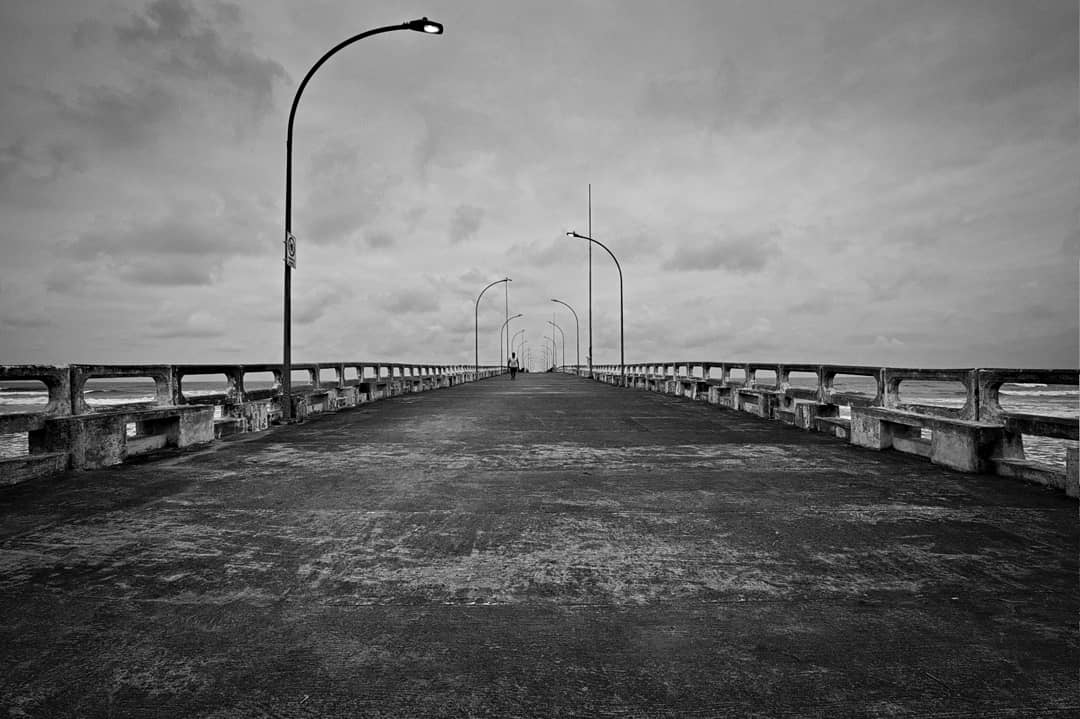
\includegraphics[scale=0.15]{plataforma.jpg}
    \caption{A plataforma de pesca.}
    \label{fig:plataforma}
\end{figure}

O argumento opcional recebe os parâmetros para escalonamento\index{escala}, dimensão\index{dimensao@dimensão}, rotação\index{rotacao@rotação} etc. Veja os exemplos:

\begin{small}
\begin{verbatim}
   \includegraphics[width=3cm, height=4cm]{logo.png}
   \includegraphics[width=\textwidth]{lua.jpg}
   \includegraphics[scale=1.2, angle=45]{foto.jpg}
\end{verbatim}
\end{small}

Por recomendação, a extensão do arquivo pode ser omitida, assim o \LaTeX\ irá procurar por todos os formatos suportados de imagens.

\subsection*{Posicionamento}
\addcontentsline{toc}{subsection}{Posicionamento}

O carregamento da imagem torna-se mais preciso se estiver no ambiente \texttt{\{figure\}}\index{figure}\index{figura}.  Pois, como já visto, com este ambiente podemos especificar o parâmetro do posicionamento\index{posicao@posição}. A imagem acima foi carregada com estas linhas de comandos:
\begin{small}
\begin{verbatim}
    \begin{figure}[h!]
        \centering
        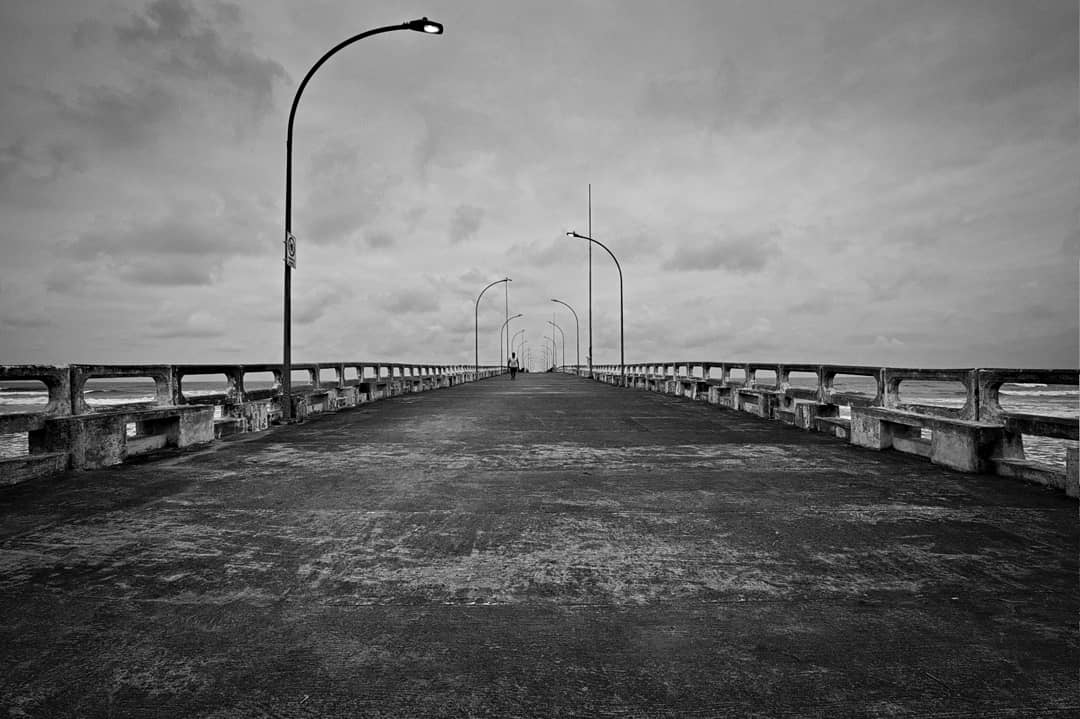
\includegraphics[scale=0.15]{plataforma.jpg}
        \caption{A plataforma de pesca.}
        \label{fig:plataforma}
    \end{figure}
\end{verbatim}
\end{small}

Adicionando o pacote \texttt{\{wrapfig\}}\index{wrapfig}, o texto ganha a possibilidade de envolver\index{envolver} a imagem carregada. Para isso usa-se o ambiente \texttt{\{wrapfigure\}}\index{wrapfigure} junto com os argumentos da posição e da largura do espaço.

Basicamente, para a posição\index{posição} existem estes parâmetros. As versões maiúsculas permitem a figura flutuar e as versões minúsculas impõem exatamente aqui:

\begin{tabular}{>{\ttfamily}l>{\ttfamily}ll}\hline
r & R & Lado direito do texto \\
l & L & Lado esquerdo do texto \\
i & I & Lado interno do encadernamento (em documento com dois lados) \\
o & O & Lado externo do encadernamento (em documento com dois lados) \\\hline
\end{tabular}

Segue uma ilustração que está, a seguir, em um exemplo de envolvimento:
\begin{small}
\begin{verbatim}
    \begin{wrapfigure}{R}{0.40\textwidth}
        \centering
        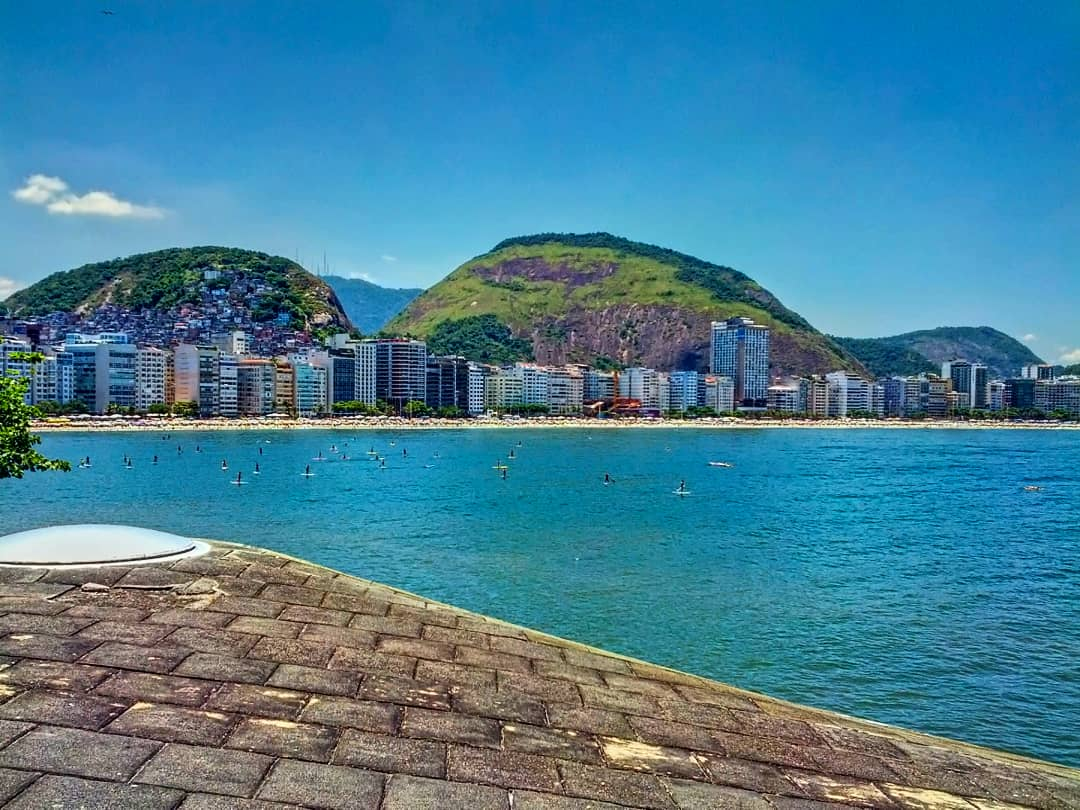
\includegraphics[width=0.35\textwidth]{copacabana.jpg}
    \end{wrapfigure}
\end{verbatim}
\end{small}

\begin{wrapfigure}{R}{0.40\textwidth}
	\centering
	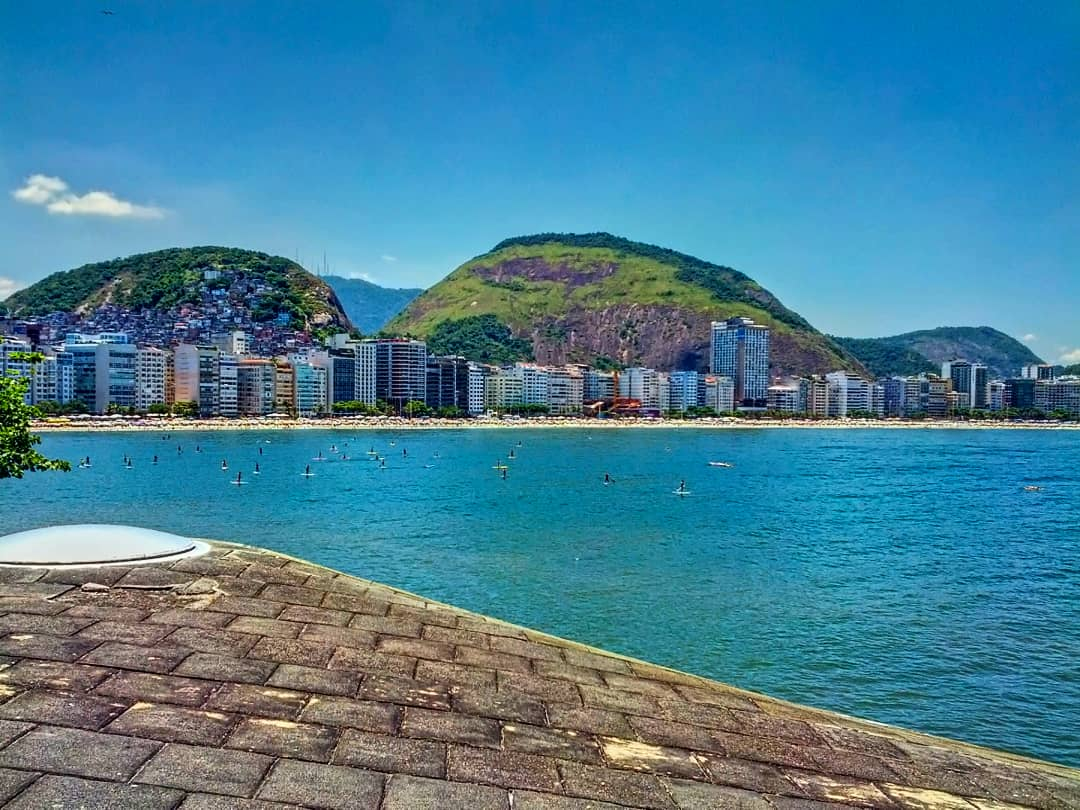
\includegraphics[width=0.35\textwidth]{copacabana.jpg}
\end{wrapfigure}

\textsl{Copacabana é um bairro situado na Zona Sul do município do Rio de Janeiro, no Brasil. É considerado um dos bairros mais famosos e prestigiados do Brasil e um dos mais conhecidos do mundo. Tem o apelido de Princesinha do Mar e Coração da Zona Sul. Faz divisa com os bairros da Lagoa, Ipanema, Botafogo, Leme e Humaitá. Copacabana atrai um grande contingente de turistas para seus mais de oitenta hotéis, que ficam especialmente cheios durante as épocas do ano-novo e do carnaval. No fim de ano, a tradicional queima de fogos na Praia de Copacabana atrai uma multidão. A orla ainda é lugar de variados eventos, como shows nacionais e internacionais, durante o resto do ano. Nos fins de semana, a faixa de areia fica cheia de moradores e de turistas. A calçada em pedras portuguesas da praia, com seu famoso desenho de ondas em padrão marlargo, ladeado pela ciclovia, é uma concorrida opção de passeio.}

%\lipsum[1-2]
%\lipsum[66]
%\lipsum[75]

\section*{Plotagem de dados}
\addcontentsline{toc}{section}{Plotagem de dados}

Baseado no pacote PGF/TikZ existe o pacote \texttt{\{pgfplots\}}\index{pgfplots}, para construir uma plotagem\index{plotagem} de dados, de funções etc. Este pacote ainda conta com um segundo componente, o pacote \texttt{\{pgfplotstable\}}\index{pgfplotstable}, que faz a formatação e o processamento de tabelas numéricas. Os ambientes de plotagem do \texttt{\{pgfplots\}} dependem do ambiente \texttt{\{tikzpicture\}}.\index{tikzpicture}\index{grafico@gráfico}

Provavelmente, o \texttt{\{pgfplots\}} é o pacote mais complexo do \LaTeX, seu manual tem quase 600 páginas, pois possui recursos tão poderosos quanto aos disponíveis nos melhores softwares matemáticos. Vale a pena a leitura do manual.

\subsection*{Configuração}
\addcontentsline{toc}{subsection}{Configuração}

Antes de executar as plotagens, é interessante configurar o \texttt{pgfplots} e isto é feito pelo comando \texttt{\textbackslash pgfplotsset}\index{pgfplotsset@\textbackslash pgfplotsset}, logo no preâmbulo ou diretamente no ambiente do gráfico.

Um primeiro ponto é quanto a compatibilidade do pacote. O \texttt{\{pgfplots\}} é desenvolvido tendo o cuidado com as versões anteriores, com os comandos que se tornaram obsoletos ou com os comandos que a sua versão instalada ainda não suporta. Por isso, inclua o parâmetro \texttt{compat=}\index{compat} mais o número da versão do pacote \texttt{\{pgfplots\}} que está instalado em seu sistema, ou uma versão anterior, se seu documento utiliza algum comando obsoleto.

O comando \texttt{\textbackslash pgfplotsset} também aceita os parâmetros de formatação do gráfico, como dimensão, estilos, fontes de caracteres etc.:

\texttt{\small\textbackslash pgfplotsset\{width=8cm, compat=1.16\}}

\subsection*{Ambientes}
\addcontentsline{toc}{subsection}{Ambientes}

Diversos ambientes irão estruturar uma plotagem, começando pelo ambiente gráfico \texttt{\{tikzpicture\}}\index{tikzpicture}, que forma a imagem. Interiormente, tem-se os ambientes específicos da plotagem, em relação aos eixos\index{eixo} de \index{escala}escala normal ou escala logarítmica\index{logaritmico@logarítmico}, com os ambientes \texttt{\{axis\}}\index{axis}, \texttt{\{semilogaxis\}}\index{semilogaxis} ou \texttt{\{loglogaxis\}}\index{loglogaxis}. Sintaxe básica:
\begin{small}
\begin{verbatim}
   \begin{tikzpicture}
      \begin{axis}[ ]
      ...
      \end{axis}
   \end{tikzpicture}
\end{verbatim}
\end{small}

Os ambientes dos eixos podem receber um argumento com os parâmetros para formatar cada eixo\index{eixo}, separados por vírgulas e seguindo a boa prática de digitá-los um por linha, por exemplo:
\begin{small}
\begin{verbatim}
   \begin{axis}[
      title = Título,
      xlabel = {$x$},
      ylabel = {$y$},
   ]
\end{verbatim}
\end{small}

Dica: Externamente ao ambiente \texttt{\{tikzpicture\}} pode-se colocar o ambiente \texttt{\{figure\}}\index{figure}, que permite, por exemplo, adicionar uma legenda\index{legenda} à figura e outros tratamentos.

\subsection*{Plotagem}
\addcontentsline{toc}{subsection}{Plotagem}

Dentro do ambiente do eixo insere-se o comando para adicionar uma plotagem\index{plotagem}, com \texttt{\textbackslash addplot}\index{addplot@\textbackslash addplot}, ou \texttt{\textbackslash addplot3}\index{addplot3@\textbackslash addplot3} para visualização em 3D\index{3d@3D}. Neste comando, especifica-se a origem dos dados\index{dados}, se será por uma função\index{funcao@função}, por coordenadas\index{coordenada} ou fornecidos por uma tabela\index{tabela} em um arquivo\index{arquivo} externo. Também pode receber um argumento com diversos parâmetros:\index{coordinates}\index{table}
\begin{small}
\begin{verbatim}
   \addplot[
      blue,
      domain=-6:4,
   ]
   {x^2 + 2*x + 1};

   \addplot[
      red,
      mark=square,
   ]
   coordinates {(1,35)(2,34)(3,30)(4,26)(5,20)(6,17)};

   \addplot table {dados.txt};
\end{verbatim}
\end{small}

O comando \texttt{\textbackslash addplot} pode ser usado mais de uma vez no mesmo gráfico\index{grafico@gráfico}, caso tenha outros dados compatíveis ao mesmo domínio.

\subsection*{Exemplos de plotagem}
\addcontentsline{toc}{subsection}{Exemplos de plotagem}

\subsubsection*{Função matemática:}

\noindent
\begin{minipage}[t]{0.5\linewidth}
\begin{small}
\begin{verbatim}
\begin{tikzpicture}
    \begin{axis}[
        axis lines = left,
        title = {Equação do 2º grau},
        xlabel = {$x$},
        ylabel = {$f(x)$},
    ]
        \addplot[domain = -6:4,
                 samples = 20,
                 color = blue,]
        {x^2 + 2*x + 1};
        \addlegendentry{$x^2 + 2x + 1$}
    \end{axis}
\end{tikzpicture}
\end{verbatim}
\end{small}
\end{minipage}\hspace{\fill}
\begin{minipage}[t]{0.4\linewidth}
\strut\vspace*{-\baselineskip}\newline
\begin{tikzpicture}
\begin{axis}[
    axis lines = left,
    title = {Equação do 2º grau},
    xlabel = {$x$},
    ylabel = {$f(x)$},
]
\addplot[
    domain = -6:4,
    samples = 20,
    color = blue,
]
{x^2 + 2*x + 1};
\addlegendentry{$x^2 + 2x + 1$}
\end{axis}
\end{tikzpicture}
\end{minipage}

\subsubsection*{Coordenadas logarítmicas:}

\noindent
\begin{minipage}[t]{0.5\linewidth}
\begin{small}
\begin{verbatim}
\begin{tikzpicture}
    \begin{loglogaxis}[
        xlabel = {Graus de liberdade},
        ylabel = {$L_2$ Erro},]

    \addplot coordinates {
        (5,8.312e-02) (49,7.407e-03)
        (321,5.874e-04) (1793,4.442e-05)
        (9217,3.261e-06) };

    \addplot coordinates {
        (7,8.472e-02) (111,1.022e-02)
        (1023,1.039e-03) (7423,9.658e-05)
        (47103,8.437e-06) };

    \legend{$d=2$,$d=3$}
    \end{loglogaxis}
\end{tikzpicture}
\end{verbatim}
\end{small}
\end{minipage}\hspace{\fill}
\begin{minipage}[t]{0.4\linewidth}
\strut\vspace*{-\baselineskip}\newline
\begin{tikzpicture}
\begin{loglogaxis}[
    xlabel = {Graus de liberdade},
    ylabel = {$L_2$ Erro},]
                   
\addplot coordinates {
	(5,8.312e-02) (49,7.407e-03)
	(321,5.874e-04) (1793,4.442e-05)
	(9217,3.261e-06)
};

\addplot coordinates {
	(7,8.472e-02) (111,1.022e-02)
	(1023,1.039e-03) (7423,9.658e-05)
	(47103,8.437e-06)
};

\legend{$d=2$,$d=3$}
\end{loglogaxis}
\end{tikzpicture}
\end{minipage}

\subsubsection*{Coordenadas em escala normal:}

\noindent
\begin{minipage}[t]{0.5\linewidth}
\begin{small}
\begin{verbatim}
\begin{tikzpicture}
\begin{axis}[
    title = {Temperaturas},
    xlabel = {Meses},
    ylabel = {°C},
    xmin = 1, xmax = 12,
    ymin = 15, ymax = 40,
    xtick = {1,2,3,4,5,6,7,8,9,10,11,12},
    ytick = {0,15,20,25,30,35,40},
    ymajorgrids = true,
    grid style = dashed,]
\addplot[blue,
         mark = square]
coordinates {
    (1,35)(2,34)(3,30)(4,26)(5,20)(6,17)
    (7,15)(8,16)(9,20)(10,26)(11,30)(12,32)};
\end{axis}
\end{tikzpicture}
\end{verbatim}
\end{small}
\end{minipage}\hspace{\fill}
\begin{minipage}[t]{0.4\linewidth}
\strut\vspace*{-\baselineskip}\newline
\begin{tikzpicture}
\begin{axis}[
    title = {Temperaturas},
    xlabel = {Meses},
    ylabel = {°C},
    xmin = 1, xmax = 12,
    ymin = 15, ymax = 40,
    xtick = {1,2,3,4,5,6,7,8,9,10,11,12},
    ytick = {0,15,20,25,30,35,40},
    ymajorgrids = true,
    grid style = dashed,]
\addplot[blue,
         mark = square]
coordinates {
	(1,35)(2,34)(3,30)(4,26)(5,20)(6,17)
	(7,15)(8,16)(9,20)(10,26)(11,30)(12,32)};
\end{axis}
\end{tikzpicture}
\end{minipage}

\subsubsection*{Plotagem em barra:}

\noindent
\begin{minipage}[t]{0.5\linewidth}
\begin{small}
\begin{verbatim}
\begin{tikzpicture}
\begin{axis}[
    ybar,
    enlargelimits = 0.3,
    legend style = {at={(0.5,-0.2)},
        anchor = north,legend columns = -1},
    ylabel = {passageiros},
    symbolic x coords={2017,2018,2019},
    xtick = data,
    nodes near coords,
    nodes near coords align={vertical},]
\addplot coordinates {(2017,7) (2018,9) (2019,5)};
\addplot coordinates {(2017,4) (2018,6) (2019,4)};
\addplot coordinates {(2017,2) (2018,2) (2019,1)};
\legend{homens,mulheres,crianças}
\end{axis}
\end{tikzpicture}
\end{verbatim}
\end{small}
\end{minipage}\hspace{\fill}
\begin{minipage}[t]{0.4\linewidth}
\strut\vspace*{-\baselineskip}\newline
\begin{tikzpicture}
\begin{axis}[
	ybar,
	enlargelimits = 0.3,
	legend style = {at={(0.5,-0.2)},
		anchor = north,legend columns = -1},
	ylabel = {passageiros},
	symbolic x coords={2017,2018,2019},
	xtick = data,
	nodes near coords,
	nodes near coords align={vertical},
]
\addplot coordinates {(2017,7) (2018,9) (2019,5)};
\addplot coordinates {(2017,4) (2018,6) (2019,4)};
\addplot coordinates {(2017,2) (2018,2) (2019,1)};
\legend{homens,mulheres,crianças}
\end{axis}
\end{tikzpicture}
\end{minipage}

\subsubsection*{Plotagem 3D:}

A plotagem em 3 dimensões é com o comando \texttt{\textbackslash addplot3}. Veja dois interessantes exemplos com os parâmetros surf e mesh, que criam uma superfície e uma malha, respectivamente:

\noindent
\begin{minipage}[t]{0.5\linewidth}
\begin{small}
\begin{verbatim}
\begin{tikzpicture}
\begin{axis}[title = {Superfície},]
\addplot3[surf, domain = 0:360,
          samples = 40,]
{sin(x)*sin(y)};
\end{axis}
\end{tikzpicture}
\end{verbatim}
\end{small}
\begin{tikzpicture}
\begin{axis}[title={Superfície},]
\addplot3[surf,
          domain=0:360,
          samples=40,]
{sin(x)*sin(y)};
\end{axis}
\end{tikzpicture}
\end{minipage}\hspace{\fill}
\begin{minipage}[t]{0.5\linewidth}
\begin{small}
\begin{verbatim}
\begin{tikzpicture}
\begin{axis}[title = Malha, hide axis,
             colormap/cool,]
\addplot3[mesh, samples = 50,
          domain = -8:8,]
{sin(deg(sqrt(x^2+y^2)))/sqrt(x^2+y^2)};
\end{axis}
\end{tikzpicture}
\end{verbatim}
\end{small}
\begin{tikzpicture}
\begin{axis}[title=Malha,
             hide axis,
             colormap/cool,]
\addplot3[mesh,
          samples=50,
          domain=-8:8,]
{sin(deg(sqrt(x^2+y^2)))/sqrt(x^2+y^2)};
\end{axis}
\end{tikzpicture}
\end{minipage}

\chapter*{Caracteres e símbolos}
\addcontentsline{toc}{chapter}{Caracteres e símbolos}

Alguns caracteres\index{caractere} acentuados\index{acento} e os caracteres de símbolos\index{simbolo@símbolo} pedem um comando específico e, normalmente, o uso de um pacote.

\section*{Acentuação}
\addcontentsline{toc}{section}{Acentuação}

Os caracteres acentuados\index{acentuacao@acentuação} podem ser digitados diretamente no documento mas, em algumas situações, é necessário usar o comando equivalente para impressão.

\subsection*{Modo texto}
\addcontentsline{toc}{subsection}{Modo texto}

Os seguintes comandos devem ser utilizados nos parágrafos ou no modo esquerda-direita (LR)\index{modolr@modo LR} e, se omitida a letra, apenas o acento é impresso:

\noindent
\begin{minipage}[t]{0.5\linewidth}
\begin{itemize}[label={}]
\setlength\itemsep{-0.5em}
\item \texttt{\textbackslash `\{a\}} grave: \`{a}
\item \texttt{\textbackslash '\{e\}} agudo: \'{e}
\item \texttt{\textbackslash \^{}\{o\}} circunflexo: \^{o}
\item \texttt{\textbackslash "\{u\}} trema: \"{u}
\item \texttt{\textbackslash H\{o\}} trema húngaro longo: \H{o}
\item \texttt{\textbackslash \~{}\{a\}} til: \~{a}
\item \texttt{\textbackslash c\{c\}} cedilha: \c{c}
\end{itemize}
\end{minipage}\hspace{\fill}
\begin{minipage}[t]{0.5\linewidth}
\begin{itemize}[label={}]
\setlength\itemsep{-0.5em}
\item \texttt{\textbackslash =\{a\}} mácron (barra em cima): \={a}
\item \texttt{\textbackslash b\{o\}} barra embaixo: \b{o}
\item \texttt{\textbackslash .\{z\}} ponto em cima: \.{z}
\item \texttt{\textbackslash d\{o\}} ponto embaixo: \d{o}
\item \texttt{\textbackslash u\{e\}} braquia (breve): \u{e}
\item \texttt{\textbackslash v\{c\}} caron: \v{c}
\item \texttt{\textbackslash t\{oo\}} braquia invertida: \t{oo}
\end{itemize}
\end{minipage}

\subsection*{Modo matemático}
\addcontentsline{toc}{subsection}{Modo matemático}

Estes, somente são aceitos no modo matemático:

\index{grave@\textbackslash grave}
\index{acute@\textbackslash acute}
\index{hat@\textbackslash hat}
\index{widehat@\textbackslash widehat}
\index{tilde@\textbackslash tilde}
\index{widetilde@\textbackslash widetilde}
\index{mathring@\textbackslash mathring}
\index{bar@\textbackslash bar}
\index{dot@\textbackslash dot}
\index{ddot@\textbackslash ddot}
\index{breve@\textbackslash breve}
\index{check@\textbackslash check}
\index{vec@\textbackslash vec}

\noindent
\begin{minipage}[t]{0.5\linewidth}
\begin{itemize}[label={}]
\setlength\itemsep{-0.5em}
\item \texttt{\textbackslash grave\{a\}} grave: $\grave{a}$
\item \texttt{\textbackslash acute\{e\}} agudo:
$\acute{e}$
\item \texttt{\textbackslash hat\{o\}} circunflexo: $\hat{o}$
\item \texttt{\textbackslash widehat\{oo\}} circunflexo largo: $\widehat{oo}$
\item \texttt{\textbackslash tilde\{a\}} til:
$\tilde{a}$
\item \texttt{\textbackslash widetilde\{aa\}} til largo: $\widetilde{aa}$
\item \texttt{\textbackslash mathring\{a\}} anel: $\mathring{a}$
\end{itemize}
\end{minipage}\hspace{\fill}
\begin{minipage}[t]{0.5\linewidth}
\begin{itemize}[label={}]
\setlength\itemsep{-0.5em}
\item \texttt{\textbackslash bar\{a\}} mácron (barra em cima):
$\bar{a}$
\item \texttt{\textbackslash dot\{z\}} ponto em cima:
$\dot{z}$
\item \texttt{\textbackslash ddot\{u\}} trema:
$\ddot{u}$
\item \texttt{\textbackslash breve\{e\}} braquia (breve):
$\breve{e}$
\item \texttt{\textbackslash check\{c\}} caron:
$\check{c}$
\item \texttt{\textbackslash vec\{v\}} vetor:
$\vec{v}$
\end{itemize}
\end{minipage}

\section*{Caracteres}
\addcontentsline{toc}{section}{Caracteres}

Além dos caracteres especiais, existem os caracteres simbólicos que, alguns por não existirem no teclado, dependem de comandos específicos para serem impressos no documento.

\subsection*{Alfabeto grego}
\addcontentsline{toc}{subsection}{Alfabeto grego}

Estes comandos nativos do \LaTeX\ funcionam somente no modo matemático.\index{alfabeto}\index{grego}

\noindent
\begin{tabular}{l>{\ttfamily\footnotesize}ll>{\ttfamily\footnotesize}ll>{\ttfamily\footnotesize}ll>{\ttfamily\footnotesize}ll>{\ttfamily\footnotesize}l}
$\alpha$
& \textbackslash alpha & 
$\beta$
& \textbackslash beta &
$\gamma$
& \textbackslash gamma & 
$\delta$
& \textbackslash delta &
$\epsilon$ & \textbackslash epsilon \\
$\varepsilon$ & \textbackslash varepsilon &
$\zeta$
& \textbackslash zeta &
$\eta$
& \textbackslash eta &
$\theta$
& \textbackslash theta &
$\vartheta$ & \textbackslash vartheta \\
$\iota$
& \textbackslash iota &
$\kappa$
& \textbackslash kappa &
$\lambda$
& \textbackslash lambda &
$\mu$
& \textbackslash mu &
$\nu$
& \textbackslash nu \\
$\xi$
& \textbackslash xi &
$\pi$
& \textbackslash pi &
$\varpi$ & \textbackslash varpi &
$\rho$
& \textbackslash rho &
$\varrho$ & \textbackslash varrho \\
$\sigma$
& \textbackslash sigma &
$\varsigma$ & \textbackslash varsigma &
$\tau$
& \textbackslash tau &
$\upsilon$
& \textbackslash upsilon &
$\phi$
& \textbackslash phi \\
$\varphi$ & \textbackslash varphi &
$\chi$
& \textbackslash chi &
$\psi$
& \textbackslash psi &
$\omega$
& \textbackslash omega &
$\Gamma$
& \textbackslash Gamma \\
$\Delta$
& \textbackslash Delta &
$\Theta$
& \textbackslash Theta &
$\Lambda$
& \textbackslash Lambda &
$\Xi$
& \textbackslash Xi &
$\Pi$
& \textbackslash Pi \\
$\Sigma$
& \textbackslash Sigma &
$\Upsilon$
& \textbackslash Upsilon &
$\Phi$
& \textbackslash Phi &
$\Psi$
& \textbackslash Psi &
$\Omega$
& \textbackslash Omega \\
\end{tabular}

\subsection*{Delimitadores de tamanho variável}
\addcontentsline{toc}{subsection}{Delimitadores de tamanho variável}

Caracteres de agrupamento\index{agrupamento} em diversos tamanhos, além dos tamanhos normais \{|[()]|\}. Estes comandos também só funcionam no modo matemático.\index{delimitador}

\index{Biggl@\textbackslash Biggl}
\index{biggl@\textbackslash biggl}
\index{Bigl@\textbackslash Bigl}
\index{bigl@\textbackslash bigl}
\index{bigr@\textbackslash bigr}
\index{Bigr@\textbackslash Bigr}
\index{biggr@\textbackslash biggr}
\index{Biggr@\textbackslash Biggr}

\begin{tabular}{r>{\ttfamily\footnotesize}lccr>{\ttfamily\footnotesize}lccr>{\ttfamily\footnotesize}lccr>{\ttfamily\footnotesize}l}
$\Biggl($ & \textbackslash Biggl( & & &
$\biggl($ & \textbackslash biggl( & & &
$\Bigl($ & \textbackslash Bigl( & & &
$\bigl($ & \textbackslash bigl( \\
$\bigr)$ & \textbackslash bigr) & & &
$\Bigr)$ & \textbackslash Bigr) & & &
$\biggr)$ & \textbackslash biggr) & & &
$\Biggr)$ & \textbackslash Biggr) \\
\arrayrulecolor{blue!50}\hdashline
$\Biggl[$ & \textbackslash Biggl[ & & &
$\biggl[$ & \textbackslash biggl[ & & &
$\Bigl[$ & \textbackslash Bigl[ & & &
$\bigl[$ & \textbackslash bigl[ \\
$\bigr]$ & \textbackslash bigr] & & &
$\Bigr]$ & \textbackslash Bigr] & & &
$\biggr]$ & \textbackslash biggr] & & &
$\Biggr]$ & \textbackslash Biggr] \\
\arrayrulecolor{blue!50}\hdashline
$\Biggl|$ & \textbackslash Biggl| & & &
$\biggl|$ & \textbackslash biggl| & & &
$\Bigl|$ & \textbackslash Bigl| & & &
$\bigl|$ & \textbackslash bigl| \\
$\bigr|$ & \textbackslash bigr| & & &
$\Bigr|$ & \textbackslash Bigr| & & &
$\biggr|$ & \textbackslash biggr| & & &
$\Biggr|$ & \textbackslash Biggr| \\
\arrayrulecolor{blue!50}\hdashline
$\Biggl\{$ & \textbackslash Biggl\textbackslash \{ & & &
$\biggl\{$ & \textbackslash biggl\textbackslash \{ & & &
$\Bigl\{$ & \textbackslash Bigl\textbackslash \{ & & &
$\bigl\{$ & \textbackslash bigl\textbackslash \{ \\
$\bigr\}$ & \textbackslash bigr\textbackslash \} & & &
$\Bigr\}$ & \textbackslash Bigr\textbackslash \} & & &
$\biggr\}$ & \textbackslash biggr\textbackslash \} & & &
$\Biggr\}$ & \textbackslash Biggr\textbackslash \} \\
\end{tabular}

\newpage
\section*{Símbolos}
\addcontentsline{toc}{section}{Símbolos}

Existem dezenas de pacotes exclusivos ao fornecimento de símbolos\index{simbolo@símbolo} e ícones\index{icone@ícone}. Alguns serão aqui apresentados resumidamente.

\subsection*{Nativos do \LaTeX\ \footnotesize{(mas alguns requerem pacote \texttt{latexsym})}}
\addcontentsline{toc}{subsection}{Nativos do \LaTeX}\index{latexsym}

\subsubsection{Operadores \footnotesize{(modo matemático)}}

\noindent\index{operador}
\begin{tabular}{l>{\ttfamily\footnotesize}ll>{\ttfamily\footnotesize}ll>{\ttfamily\footnotesize}ll>{\ttfamily\footnotesize}l}
$\amalg$ & \textbackslash amalg &
$\ast$ & \textbackslash ast &
$\bigcirc$ & \textbackslash bigcirc &
$\bigtriangledown$ & \textbackslash bigtriangledown \\
$\bigtriangleup$ & \textbackslash bigtriangleup &
$\bullet$ & \textbackslash bullet &
$\cdot$ & \textbackslash cdot &
$\circ$ & \textbackslash circ \\
$\dagger$ & \textbackslash dagger &
$\ddagger$ & \textbackslash ddagger &
$\diamond$ &\textbackslash diamond &
$\div$ & \textbackslash div \\
$\lhd$ & \textbackslash lhd &
$\mp$ & \textbackslash mp &
$\odot$ & \textbackslash odot &
$\ominus$ & \textbackslash ominus \\
$\oplus$ & \textbackslash oplus &
$\oslash$ & \textbackslash oslash &
$\otimes$ & \textbackslash otimes &
$\pm$ & \textbackslash pm \\
$\rhd$ & \textbackslash rhd &
$\setminus$ & \textbackslash setminus &
$\sqcap$ & \textbackslash sqcap &
$\sqcup$ & \textbackslash sqcup \\
$\star$ & \textbackslash star &
$\times$ & \textbackslash times &
$\triangleleft$ & \textbackslash triangleleft &
$\triangleright$ & \textbackslash triangleright \\
$\unlhd$ & \textbackslash unlhd &
$\unrhd$ & \textbackslash unrhd &
$\uplus$ & \textbackslash uplus &
$\vee$ & \textbackslash vee \\
$\wedge$ & \textbackslash wedge &
$\wr$ & \textbackslash wr \\
\end{tabular}

\subsubsection{Operadores de tamanho variável \footnotesize{(modo matemático)}}

\noindent
\begin{tabular}{l>{\ttfamily\footnotesize}ll>{\ttfamily\footnotesize}ll>{\ttfamily\footnotesize}ll>{\ttfamily\footnotesize}ll>{\ttfamily\footnotesize}l}
$\bigcap$ & \textbackslash bigcap &
$\bigcup$ & \textbackslash bigcup &
$\bigodot$ & \textbackslash bigodot &
$\bigoplus$ & \textbackslash bigoplus &
$\bigotimes$ & \textbackslash bigotimes \\
$\bigsqcup$ & \textbackslash bigsqcup &
$\biguplus$ & \textbackslash biguplus &
$\bigvee$ & \textbackslash bigvee &
$\bigwedge$ & \textbackslash bigwedge &
$\coprod$ & \textbackslash coprod \\
$\int$ & \textbackslash int &
$\oint$ & \textbackslash oint &
$\prod$ & \textbackslash prod &
$\sum$ & \textbackslash sum \\
\end{tabular}

\subsubsection{Setas \footnotesize{(modo matemático)}}

\noindent\index{seta}
\begin{tabular}{l>{\ttfamily\footnotesize}ll>{\ttfamily\footnotesize}ll>{\ttfamily\footnotesize}l}
$\Downarrow$ & \textbackslash Downarrow &
$\downarrow$ & \textbackslash downarrow &
$\hookleftarrow$ & \textbackslash hookleftarrow \\
$\hookrightarrow$ & \textbackslash hookrightarrow &
$\leadsto$ & \textbackslash leadsto &
$\leftarrow$ & \textbackslash leftarrow \\
$\Leftarrow$ & \textbackslash Leftarrow &
$\Leftrightarrow$ & \textbackslash Leftrightarrow &
$\leftrightarrow$ & \textbackslash leftrightarrow \\
$\longleftarrow$ & \textbackslash longleftarrow &
$\Longleftarrow$ & \textbackslash Longleftarrow &
$\longleftrightarrow$ & \textbackslash longleftrightarrow \\
$\Longleftrightarrow$ & \textbackslash Longleftrightarrow &
$\longmapsto$ & \textbackslash longmapsto &
$\Longrightarrow$ & \textbackslash Longrightarrow \\
$\longrightarrow$ & \textbackslash longrightarrow &
$\mapsto$ & \textbackslash mapsto &
$\nearrow$ & \textbackslash nearrow \\
$\nwarrow$ & \textbackslash nwarrow &
$\Rightarrow$ & \textbackslash Rightarrow &
$\rightarrow$ & \textbackslash rightarrow \\
$\searrow$ & \textbackslash searrow &
$\swarrow$ & \textbackslash swarrow &
$\uparrow$ & \textbackslash uparrow \\
$\Uparrow$ & \textbackslash Uparrow &
$\updownarrow$ & \textbackslash updownarrow &
$\Updownarrow$ & \textbackslash Updownarrow \\
\end{tabular}

\subsubsection{Desigualdades \footnotesize{(modo matemático)}}

\noindent\index{desigualdade}
\begin{tabular}{l>{\ttfamily\footnotesize}lcl>{\ttfamily\footnotesize}lcl>{\ttfamily\footnotesize}lcl>{\ttfamily\footnotesize}lcl>{\ttfamily\footnotesize}l}
$\geq$ & \textbackslash geq & &
$\gg$ & \textbackslash gg & &
$\leq$ & \textbackslash leq & &
$\ll$ & \textbackslash ll & &
$\neq$ & \textbackslash neq \\
\end{tabular}

\subsubsection{Relações binárias \footnotesize{(modo matemático)}}

\noindent
\begin{tabular}{l>{\ttfamily\footnotesize}ll>{\ttfamily\footnotesize}ll>{\ttfamily\footnotesize}ll>{\ttfamily\footnotesize}ll>{\ttfamily\footnotesize}ll>{\ttfamily\footnotesize}l}
$\approx$ & \textbackslash approx &
$\asymp$ & \textbackslash asymp &
$\bowtie$ & \textbackslash bowtie &
$\cong$ & \textbackslash cong &
$\dashv$ & \textbackslash dashv &
$\doteq$ & \textbackslash doteq \\
$\equiv$ & \textbackslash equiv &
$\frown$ & \textbackslash frown &
$\Join$ & \textbackslash Join &
$\mid$ & \textbackslash mid &
$\models$ & \textbackslash models &
$\parallel$ & \textbackslash parallel \\
$\perp$ & \textbackslash perp &
$\prec$ & \textbackslash prec &
$\preceq$ & \textbackslash preceq &
$\propto$ & \textbackslash propto &
$\sim$ & \textbackslash sim &
$\simeq$ & \textbackslash simeq \\
$\smile$ & \textbackslash smile &
$\succ$ & \textbackslash succ &
$\succeq$ & \textbackslash succeq &
$\vdash$ & \textbackslash vdash \\
\end{tabular}

\subsubsection{Funções matemáticas \footnotesize{(modo matemático)}}

\noindent\index{funcoes@funções}
\begin{tabular}{l>{\ttfamily\footnotesize}ll>{\ttfamily\footnotesize}ll>{\ttfamily\footnotesize}ll>{\ttfamily\footnotesize}ll>{\ttfamily\footnotesize}l}
$\arccos$ & \textbackslash arccos &
$\cos$ & \textbackslash cos &
$\csc$ & \textbackslash csc &
$\exp$ & \textbackslash exp &
$\ker$ & \textbackslash ker \\
$\limsup$ & \textbackslash limsup &
$\min$ & \textbackslash min &
$\sinh$ & \textbackslash sinh &
$\arcsin$ & \textbackslash arcsin &
$\cosh$ & \textbackslash cosh \\
$\deg$ & \textbackslash deg &
$\gcd$ & \textbackslash gcd &
$\lg$ & \textbackslash lg &
$\ln$ & \textbackslash ln &
$\Pr$ & \textbackslash Pr \\
$\sup$ & \textbackslash sup &
$\arctan$ & \textbackslash arctan &
$\cot$ & \textbackslash cot &
$\det$ & \textbackslash det &
$\hom$ & \textbackslash hom \\
$\lim$ & \textbackslash lim &
$\log$ & \textbackslash log &
$\sec$ & \textbackslash sec &
$\tan$ & \textbackslash tan &
$\arg$ & \textbackslash arg \\
$\coth$ & \textbackslash coth &
$\dim$ & \textbackslash dim &
$\inf$ & \textbackslash inf &
$\liminf$ & \textbackslash liminf &
$\max$ & \textbackslash max \\
$\sin$ & \textbackslash sin &
$\tanh$ & \textbackslash tanh \\
\end{tabular}

\subsubsection{Acentos extensíveis \footnotesize{(modo matemático)}}

\noindent\index{acento}
\begin{tabular}{l>{\ttfamily\footnotesize}ll>{\ttfamily\footnotesize}ll>{\ttfamily\footnotesize}l}
$\widetilde{abc}$ & \textbackslash widetilde\{abc\} &
$\widehat{abc}$ & \textbackslash widehat\{abc\} &
$\overleftarrow{abc}$ & \textbackslash overleftarrow\{abc\} \\
$\overrightarrow{abc}$ & \textbackslash overrightarrow\{abc\} &
$\overline{abc}$ & \textbackslash overline\{abc\} &
$\underline{abc}$ & \textbackslash underline\{abc\} \\
$\overbrace{abc}$ & \textbackslash overbrace\{abc\} &
$\underbrace{abc}$ & \textbackslash underbrace\{abc\} &
$\sqrt{abc}$ & \textbackslash sqrt\{abc\} \\
\end{tabular}

\subsubsection{Relações de conjuntos \footnotesize{(modo matemático)}}

\noindent\index{conjunto}
\begin{tabular}{l>{\ttfamily\footnotesize}lcl>{\ttfamily\footnotesize}lcl>{\ttfamily\footnotesize}lcl>{\ttfamily\footnotesize}l}
$\in$ & \textbackslash in & &
$\ni$ & \textbackslash ni & &
$\cap$ & \textbackslash cap & &
$\cup$ & \textbackslash cup \\
$\subset$ & \textbackslash subset & &
$\supset$ & \textbackslash supset & &
$\subseteq$ & \textbackslash subseteq & &
$\supseteq$ & \textbackslash supseteq \\
$\sqsubset$ & \textbackslash sqsubset & &
$\sqsupset$ & \textbackslash sqsupset & &
$\sqsubseteq$ & \textbackslash sqsubseteq & &
$\sqsupseteq$ & \textbackslash sqsupseteq \\
$\exists$ & \textbackslash exists & &
$\forall$ & \textbackslash forall \\
\end{tabular}

\subsubsection{Símbolos diversos \footnotesize{(modo matemático)}}

\noindent\index{simbolo@símbolo}
\begin{tabular}{l>{\ttfamily\footnotesize}lcl>{\ttfamily\footnotesize}lcl>{\ttfamily\footnotesize}lcl>{\ttfamily\footnotesize}l}
$\bot$ & \textbackslash bot & &
$\ell$ & \textbackslash ell & &
$\hbar$ & \textbackslash hbar & &
$\Im$ & \textbackslash Im \\
$\imath$ & \textbackslash imath & &
$\jmath$ & \textbackslash jmath & &
$\partial$ & \textbackslash partial & &
$\Re$ & \textbackslash Re \\
$\top$ & \textbackslash top & &
$\wp$ & \textbackslash wp & &
$\aleph$ & \textbackslash aleph & &
$\emptyset$ & \textbackslash emptyset \\
$\angle$ & \textbackslash angle & &
$\backslash$ & \textbackslash backslash & &
$\Box$ & \textbackslash Box & &
$\Diamond$ & \textbackslash Diamond \\
$\infty$ & \textbackslash infty & &
$\mho$ & \textbackslash mho & &
$\nabla$ & \textbackslash nabla & &
$\neg$ & \textbackslash neg \\
$\prime$ & \textbackslash prime & &
$\surd$ & \textbackslash surd & &
$\triangle$ & \textbackslash triangle & &
$\flat$ & \textbackslash flat \\
$\natural$ & \textbackslash natural & &
$\sharp$ & \textbackslash sharp & &
$\clubsuit$ & \textbackslash clubsuit & &
$\diamondsuit$ & \textbackslash diamondsuit \\
$\heartsuit$ & \textbackslash heartsuit & &
$\spadesuit$ & \textbackslash spadesuit & &
$\copyright$ & \textbackslash copyright & &
$\dag$ & \textbackslash dag \\
$\ddag$ & \textbackslash ddag & &
$\dots$ & \textbackslash dots & &
$\P$ & \textbackslash P & &
$\pounds$ & \textbackslash pounds \\
$\S$ & \textbackslash S & &
$\$$ & \textbackslash\$ \\
\end{tabular}

\subsubsection{Pontos \footnotesize{(modo matemático)}}

\noindent\index{ponto}
\begin{tabular}{l>{\ttfamily\footnotesize}lccl>{\ttfamily\footnotesize}lccl>{\ttfamily\footnotesize}lccl>{\ttfamily\footnotesize}l}
$\cdotp$ & \textbackslash cdotp & & &
$\colon$ & \textbackslash colon & & &
$\ldotp$ & \textbackslash ldotp & & &
$\vdots$ & \textbackslash vdots \\
$\cdots$ & \textbackslash cdots & & &
$\ddots$ & \textbackslash ddots & & &
$\ldots$ & \textbackslash ldots \\
\end{tabular}

\subsubsection{Modo texto}

\noindent\index{modotexto@modo texto}
\begin{tabular}{l>{\ttfamily\footnotesize}ll>{\ttfamily\footnotesize}ll>{\ttfamily\footnotesize}l}
\textbackslash & \textbackslash textbackslash &
\textbar & \textbackslash textbar &
\textbardbl & \textbackslash textbardbl \\
\textbigcircle & \textbackslash textbigcircle &
\textbullet & \textbackslash textbullet &
\textdagger & \textbackslash textdagger \\
\textdaggerdbl & \textbackslash textdaggerdbl &
\textellipsis & \textbackslash textellipsis &
\textemdash & \textbackslash textemdash \\
\textendash & \textbackslash textendash &
\textexclamdown & \textbackslash textexclamdown &
\textgreater & \textbackslash textgreater \\
\textless & \textbackslash textless &
\textordfeminine & \textbackslash textordfeminine &
\textordmasculine & \textbackslash textordmasculine \\
\textparagraph & \textbackslash textparagraph &
\textperiodcentered & \textbackslash textperiodcentered &
\textpertenthousand & \textbackslash textpertenthousand \\
\textperthousand & \textbackslash textperthousand &
\textquestiondown & \textbackslash textquestiondown &
\textquotedblleft & \textbackslash textquotedblleft \\
\textquotedblright & \textbackslash textquotedblright &
\textquoteleft & \textbackslash textquoteleft &
\textquoteright & \textbackslash textquoteright \\
\textsection & \textbackslash textsection &
\textunderscore & \textbackslash textunderscore &
\textvisiblespace & \textbackslash textvisiblespace \\
\copyright & \textbackslash copyright &
\dag & \textbackslash dag &
\ddag & \textbackslash ddag \\
\dots & \textbackslash dots &
\P & \textbackslash P &
\pounds & \textbackslash pounds \\
\S & \textbackslash S &
\$ & \textbackslash\$ \\
\end{tabular}

\subsection*{Text Companion \footnotesize{(pacote \texttt{textcomp})}}
\addcontentsline{toc}{subsection}{Text Companion}\index{textcomp}

\noindent\index{textcompanion@Text Companion}
\begin{tabular}{l>{\ttfamily\footnotesize}ll>{\ttfamily\footnotesize}ll>{\ttfamily\footnotesize}l}
\textdownarrow & \textbackslash textdownarrow &
\textrightarrow & \textbackslash textrightarrow &
\textleftarrow & \textbackslash textleftarrow \\
\textuparrow & \textbackslash textuparrow &
\textdollar & \textbackslash textdollar &
\textsterling & \textbackslash textsterling \\
\texteuro & \textbackslash texteuro &
\textcent & \textbackslash textcent &
\textwon & \textbackslash textwon \\
\textyen & \textbackslash textyen &
\textpeso & \textbackslash textpeso &
\textcurrency & \textbackslash textcurrency \\
\textcircledP & \textbackslash textcircledP &
\textcopyright & \textbackslash textcopyright &
\textregistered & \textbackslash textregistered \\
\textservicemark & \textbackslash textservicemark &
\texttrademark & \textbackslash texttrademark &
\textcelsius & \textbackslash textcelsius \\
\textmho & \textbackslash textmho &
\textmu & \textbackslash textmu &
\textohm & \textbackslash textohm \\
\textacutedbl & \textbackslash textacutedbl &
\textasciicaron & \textbackslash textasciicaron &
\textasciimacron & \textbackslash textasciimacron \\
\textasciiacute & \textbackslash textasciiacute &
\textasciidieresis & \textbackslash textasciidieresis &
\textgravedbl & \textbackslash textgravedbl \\
\textasciibreve & \textbackslash textasciibreve &
\textasciigrave & \textbackslash textasciigrave &
\textbrokenbar & \textbackslash textbrokenbar \\
\textdiscount & \textbackslash textdiscount &
\textestimated & \textbackslash textestimated &
\textnumero & \textbackslash textnumero \\
\textopenbullet & \textbackslash textopenbullet &
\textquotesingle & \textbackslash textquotesingle &
\textquotestraightbase & \textbackslash textquotestraightbase \\
\textquotestraightdblbase & \textbackslash textquotestraightdblbase &
\textrecipe & \textbackslash textrecipe &
\textreferencemark & \textbackslash textreferencemark \\
\texttildelow & \textbackslash texttildelow &
\textblank & \textbackslash textblank &
\textpilcrow & \textbackslash textpilcrow \\
\textlangle & \textbackslash textlangle &
\textrangle & \textbackslash textrangle &
\textlbrackdbl & \textbackslash textlbrackdbl \\
\textrbrackdbl & \textbackslash textrbrackdbl &
\textlquill & \textbackslash textlquill &
\textrquill & \textbackslash textrquill \\
\textdegree & \textbackslash textdegree &
\textlnot & \textbackslash textlnot &
\textminus & \textbackslash textminus \\
\texttimes & \textbackslash texttimes &
\textdiv & \textbackslash textdiv &
\textpm & \textbackslash textpm \\
\textonesuperior & \textbackslash textonesuperior &
\texttwosuperior & \textbackslash texttwosuperior &
\textthreesuperior & \textbackslash textthreesuperior \\
\textsurd & \textbackslash textsurd &
\textmusicalnote & \textbackslash textmusicalnote &
\textborn & \textbackslash textborn \\
\textdied & \textbackslash textdied &
\textmarried & \textbackslash textmarried &
\textdivorced & \textbackslash textdivorced \\
\end{tabular}

\newpage
\subsection*{American Mathematical Society \footnotesize{(pacotes \texttt{amsmath} e \texttt{amssymb})}}
\addcontentsline{toc}{subsection}{American Mathematical Society}\index{amsmath}\index{amssymb}

Obs.: Estes comandos funcionam no modo matemático.

\noindent\index{ams@AMS}
\begin{tabular}{l>{\ttfamily\footnotesize}ll>{\ttfamily\footnotesize}ll>{\ttfamily\footnotesize}l}
$\leftarrowtail$ & \textbackslash leftarrowtail &
$\rightarrowtail$ & \textbackslash rightarrowtail &
$\looparrowleft$ & \textbackslash looparrowleft \\
$\looparrowright$ & \textbackslash looparrowright &
$\Rsh$ & \textbackslash Rsh &
$\Lsh$ & \textbackslash Lsh \\
$\curvearrowleft$ & \textbackslash curvearrowleft &
$\curvearrowright$ & \textbackslash curvearrowright &
$\circlearrowleft$ & \textbackslash circlearrowleft \\
$\circlearrowright$ & \textbackslash circlearrowright &
$\upharpoonright$ & \textbackslash upharpoonright &
$\upharpoonleft$ & \textbackslash upharpoonleft \\
$\downharpoonright$ & \textbackslash downharpoonright &
$\downharpoonleft$ & \textbackslash downharpoonleft &
$\rightleftarrows$ & \textbackslash rightleftarrows \\
$\leftrightarrows$ & \textbackslash leftrightarrows &
$\leftleftarrows$ & \textbackslash leftleftarrows &
$\upuparrows$ & \textbackslash upuparrows \\
$\rightrightarrows$ & \textbackslash rightrightarrows &
$\downdownarrows$ & \textbackslash downdownarrows &
$\leftrightharpoons$ & \textbackslash leftrightharpoons \\
$\rightleftharpoons$ & \textbackslash rightleftharpoons &
$\Lleftarrow$ & \textbackslash Lleftarrow &
$\Rrightarrow$ & \textbackslash Rrightarrow \\
$\nexists$ & \textbackslash nexists &
$\varnothing$ & \textbackslash varnothing &
$\measuredangle$ & \textbackslash measuredangle \\
$\sphericalangle$ & \textbackslash sphericalangle &
$\nmid$ & \textbackslash nmid &
$\nparallel$ & \textbackslash nparallel \\
$\wedge$ & \textbackslash wedge &
$\therefore$ & \textbackslash therefore &
$\because$ & \textbackslash because \\
$\backsim$ & \textbackslash backsim &
$\wr$ & \textbackslash wr &
$\nsim$ & \textbackslash nsim \\
$\eqsim$ & \textbackslash eqsim &
$\ncong$ & \textbackslash ncong &
$\approxeq$ & \textbackslash approxeq \\
$\leqq$ & \textbackslash leqq &
$\geqq$ & \textbackslash geqq &
$\lneqq$ & \textbackslash lneqq \\
$\gneqq$ & \textbackslash gneqq &
$\between$ & \textbackslash between &
$\nless$ & \textbackslash nless \\
$\ngtr$ & \textbackslash ngtr &
$\nleq$ & \textbackslash nleq &
$\ngeq$ & \textbackslash ngeq \\
$\lesssim$ & \textbackslash lesssim &
$\gtrsim$ & \textbackslash gtrsim &
$\lessgtr$ & \textbackslash lessgtr \\
$\gtrless$ & \textbackslash gtrless &
$\nsubseteq$ & \textbackslash nsubseteq &
$\nsupseteq$ & \textbackslash nsupseteq \\
$\subsetneq$ & \textbackslash subsetneq &
$\supsetneq$ & \textbackslash supsetneq &
$\circledcirc$ & \textbackslash circledcirc \\
$\boxplus$ & \textbackslash boxplus &
$\boxminus$ & \textbackslash boxminus &
$\boxtimes$ & \textbackslash boxtimes \\
$\boxdot$ & \textbackslash boxdot &
$\dashv$ & \textbackslash dashv &
$\vDash$ & \textbackslash vDash \\
$\Vdash$ & \textbackslash Vdash &
$\Vvdash$ & \textbackslash Vvdash &
$\nvdash$ & \textbackslash nvdash \\
$\nvDash$ & \textbackslash nvDash &
$\nVdash$ & \textbackslash nVdash &
$\nVDash$ & \textbackslash nVDash \\
$\vartriangleleft$ & \textbackslash vartriangleleft &
$\vartriangleright$ & \textbackslash vartriangleright &
$\multimap$ & \textbackslash multimap \\
$\intercal$ & \textbackslash intercal &
$\ltimes$ & \textbackslash ltimes &
$\rtimes$ & \textbackslash rtimes \\
$\leftthreetimes$ & \textbackslash leftthreetimes &
$\rightthreetimes$ & \textbackslash rightthreetimes &
$\backsimeq$ & \textbackslash backsimeq \\
$\curlyvee$ & \textbackslash curlyvee &
$\curlywedge$ & \textbackslash curlywedge &
$\lessdot$ & \textbackslash lessdot \\
$\gtrdot$ & \textbackslash gtrdot &
$\lll$ & \textbackslash lll &
$\ggg$ & \textbackslash ggg \\
$\lesseqgtr$ & \textbackslash lesseqgtr &
$\gtreqless$ & \textbackslash gtreqless &
%$\Diamond$ & \textbackslash Diamond \\
%$\lozenge$ & \textbackslash lozenge &
%$\square$ & \textbackslash square &
%$\blacksquare$ & \textbackslash blacksquare \\
%$\bigstar$ & \textbackslash bigstar &
$\Join$ & \textbackslash Join \\
$\leqslant$ & \textbackslash leqslant &
$\geqslant$ & \textbackslash geqslant &
$\lessapprox$ & \textbackslash lessapprox \\
$\gtrapprox$ & \textbackslash gtrapprox &
$\lneq$ & \textbackslash lneq &
$\gneq$ & \textbackslash gneq \\
$\lnapprox$ & \textbackslash lnapprox &
$\gnapprox$ & \textbackslash gnapprox &
$\lesseqqgtr$ & \textbackslash lesseqqgtr \\
$\gtreqqless$ & \textbackslash gtreqqless &
$\subseteqq$ & \textbackslash subseteqq &
$\supseteqq$ & \textbackslash supseteqq \\
$\subsetneqq$ & \textbackslash subsetneqq &
$\supsetneqq$ & \textbackslash supsetneqq &
$\varkappa$ & \textbackslash varkappa \\
$\implies$ & \textbackslash implies &
$\checkmark$ & \textbackslash checkmark &
%$\circledR$ & \textbackslash circledR &
$\maltese$ & \textbackslash maltese \\
$\ulcorner$ & \textbackslash ulcorner &
$\urcorner$ & \textbackslash urcorner &
$\llcorner$ & \textbackslash llcorner \\
$\lrcorner$ & \textbackslash lrcorner &
$\mathbb{N}$ & \textbackslash mathbb\{N\} &
$\mathbb{Z}$ & \textbackslash mathbb\{Z\} \\
$\mathbb{Q}$ & \textbackslash mathbb\{Q\} &
$\mathbb{R}$ & \textbackslash mathbb\{R\} &
$\mathbb{C}$ & \textbackslash mathbb\{C\} \\
$\dotsb$ & \textbackslash dotsb &
$\dotsc$ & \textbackslash dotsc &
$\dotsi$ & \textbackslash dotsi \\
$\dotsm$ & \textbackslash dotsm &
$\dotso$ & \textbackslash dotso \\
\end{tabular}

O pacote \texttt{\{amsmath\}} tem o comando \texttt{\textbackslash text\{\}} o qual aplica a formatação do ambiente externo, e ainda \texttt{\textbackslash mathrm\{\}}, \texttt{\textbackslash mathsf\{\}}, \texttt{\textbackslash mathbf\{\}}, \texttt{\textbackslash mathtt\{\}} e \texttt{\textbackslash mathit\{\}}.\index{romano}\index{semserifa@sem serifa}\index{negrito}\index{teletipo}\index{teletype}\index{italico@itálico}

\subsection*{Font Awesome \footnotesize{(pacote \texttt{fontawesome})}}
\addcontentsline{toc}{subsection}{Font Awesome}\index{fontawesome}

\noindent\index{fontawesome@Font Awesome}
\begin{tabular}{l>{\ttfamily\footnotesize}ll>{\ttfamily\footnotesize}ll>{\ttfamily\footnotesize}l}
\faFacebook & \textbackslash faFacebook &
\faInstagram & \textbackslash faInstagram &
\faTwitter & \textbackslash faTwitter \\
\faLinkedin & \textbackslash faLinkedin &
\faPinterest & \textbackslash faPinterest &
\faReddit & \textbackslash faReddit \\
\faFoursquare & \textbackslash faFoursquare &
\faTumblr & \textbackslash faTumblr &
\faAmazon & \textbackslash faAmazon \\
\faVimeo & \textbackslash faVimeo &
\faYoutube & \textbackslash faYoutube &
\faYelp & \textbackslash faYelp \\
\faDropbox & \textbackslash faDropbox &
\faGithub & \textbackslash faGithub &
\faGoogle & \textbackslash faGoogle \\
\faSkype & \textbackslash faSkype &
\faLinux & \textbackslash faLinux &
\faAndroid & \textbackslash faAndroid \\
\faWindows & \textbackslash faWindows &
\faApple & \textbackslash faApple &
\faFirefox & \textbackslash faFirefox \\
\faChrome & \textbackslash faChrome &
\faOpera & \textbackslash faOpera &
\faInternetExplorer & \textbackslash faInternetExplorer \\
\faFloppyO & \textbackslash faFloppyO &
\faHddO & \textbackslash faHddO &
\faMousePointer & \textbackslash faMousePointer \\
\faSpotify & \textbackslash faSpotify &
\faSoundcloud & \textbackslash faSoundcloud &
\faHeadphones & \textbackslash faHeadphones \\
\faMicrophone & \textbackslash faMicrophone &
\faThumbsOUp & \textbackslash faThumbsOUp &
\faThumbsODown & \textbackslash faThumbsODown \\
\faHandORight & \textbackslash faHandORight &
\faHandOLeft & \textbackslash faHandOLeft &
\faArrowDown & \textbackslash faArrowDown \\
\faArrowUp & \textbackslash faArrowUp &
\faArrowLeft & \textbackslash faArrowLeft &
\faArrowRight & \textbackslash faArrowRight \\
\faChevronCircleDown & \textbackslash faChevronCircleDown &
\faChevronCircleUp & \textbackslash faChevronCircleUp &
\faChevronCircleLeft & \textbackslash faChevronCircleLeft \\
\faChevronCircleRight & \textbackslash faChevronCircleRight &
\faStar & \textbackslash faStar &
\faStarHalf & \textbackslash faStarHalf \\
\faStarHalfO & \textbackslash faStarHalfO &
\faStarO & \textbackslash faStarO &
\faCircle & \textbackslash faCircle \\
\faCircleO & \textbackslash faCircleO &
\faSquare & \textbackslash faSquare &
\faSquareO & \textbackslash faSquareO \\
\faMale & \textbackslash faMale &
\faFemale & \textbackslash faFemale &
\faCheck & \textbackslash faCheck \\
\faClose & \textbackslash faClose &
\faRecycle & \textbackslash faRecycle &
\faPowerOff & \textbackslash faPowerOff \\
\faSignal & \textbackslash faSignal &
\faWifi & \textbackslash faWifi &
\faBatteryEmpty & \textbackslash faBatteryEmpty \\
\faBatteryFull & \textbackslash faBatteryFull &
\faBatteryHalf & \textbackslash faBatteryHalf &
\faBatteryQuarter & \textbackslash faBatteryQuarter \\
\faSortAlphaAsc & \textbackslash faSortAlphaAsc &
\faSortAlphaDesc & \textbackslash faSortAlphaDesc &
\faSortNumericAsc & \textbackslash faSortNumericAsc \\
\faSortNumericDesc & \textbackslash faSortNumericDesc &
\faCcVisa & \textbackslash faCcVisa &
\faCcMastercard & \textbackslash faCcMastercard \\
\faCcAmex & \textbackslash faCcAmex &
\faCcDinersClub & \textbackslash faCcDinersClub &
\faFutbolO & \textbackslash faFutbolO \\
\faScissors & \textbackslash faScissors &
\faPhone & \textbackslash faPhone &
\faShoppingCart & \textbackslash faShoppingCart \\
\faAngleDown & \textbackslash faAngleDown &
\faAngleLeft & \textbackslash faAngleLeft &
\faAngleRight & \textbackslash faAngleRight \\
\faAngleUp & \textbackslash faAngleUp &
\faAngleDoubleDown & \textbackslash faAngleDoubleDown &
\faAngleDoubleLeft & \textbackslash faAngleDoubleLeft \\
\faAngleDoubleRight & \textbackslash faAngleDoubleRight &
\faAngleDoubleUp & \textbackslash faAngleDoubleUp &
\faRefresh & \textbackslash faRefresh \\
\faBan & \textbackslash faBan &
\faRocket & \textbackslash faRocket &
\faRss & \textbackslash faRss \\
\faSearch & \textbackslash faSearch &
\faSearchMinus & \textbackslash faSearchMinus &
\faSearchPlus & \textbackslash faSearchPlus \\
\faShare & \textbackslash faShare &
\faShareAlt & \textbackslash faShareAlt &
\faBell & \textbackslash faBell \\
\faBellO & \textbackslash faBellO &
\faShield & \textbackslash faShield &
\faBinoculars & \textbackslash faBinoculars \\
\faBolt & \textbackslash faBolt &
\faBook & \textbackslash faBook &
\faSliders & \textbackslash faSliders \\
\faHeart & \textbackslash faHeart &
\faHeartbeat & \textbackslash faHeartbeat &
\faHeartO & \textbackslash faHeartO \\
\faHistory & \textbackslash faHistory &
\faHome & \textbackslash faHome &
\faCalendar & \textbackslash faCalendar \\
\faCalculator & \textbackslash faCalculator &
\faHourglassEnd & \textbackslash faHourglassEnd &
\faHourglassHalf & \textbackslash faHourglassHalf \\
\faHourglassStart & \textbackslash faHourglassStart &
\faCamera & \textbackslash faCamera &
\faCar & \textbackslash faCar \\
\faBicycle & \textbackslash faBicycle &
\faMotorcycle & \textbackslash faMotorcycle &
\faBus & \textbackslash faBus \\
\faTrain & \textbackslash faTrain &
\faAmbulance & \textbackslash faAmbulance &
\faPlane & \textbackslash faPlane \\
\faTree & \textbackslash faTree &
\faUmbrella & \textbackslash faUmbrella &
\faDiamond & \textbackslash faDiamond \\
\faDatabase & \textbackslash faDatabase &
\faCube & \textbackslash faCube &
\faDownload & \textbackslash faDownload \\
\faEnvelope & \textbackslash faEnvelope &
\faEnvelopeO & \textbackslash faEnvelopeO &
\faPaperclip & \textbackslash faPaperclip \\
\faPaperPlane & \textbackslash faPaperPlane &
\faPaperPlaneO & \textbackslash faPaperPlaneO &
\faPaw & \textbackslash faPaw \\
\faPlay & \textbackslash faPlay &
\faStop & \textbackslash faStop &
\faBackward & \textbackslash faBackward \\
\faForward & \textbackslash faForward &
\faFastBackward & \textbackslash faFastBackward &
\faFastForward & \textbackslash faFastForward \\
\end{tabular}

\subsection*{Zapf Dingbats \footnotesize{(pacote \texttt{pifont})}}
\addcontentsline{toc}{subsection}{Zapf Dingbats}\index{pifont}

Obs.: Estes comandos funcionam no modo texto.\index{zapfdingbats@Zapf Dingbats}

\noindent
\begin{tabular}{l>{\ttfamily\footnotesize}ll>{\ttfamily\footnotesize}ll>{\ttfamily\footnotesize}ll>{\ttfamily\footnotesize}ll>{\ttfamily\footnotesize}l}
\ding{34} & \textbackslash ding\{34\} &
\ding{36} & \textbackslash ding\{36\} &
\ding{42} & \textbackslash ding\{42\} &
\ding{43} & \textbackslash ding\{43\} &
\ding{44} & \textbackslash ding\{44\} \\
\ding{45} & \textbackslash ding\{45\} &
\ding{46} & \textbackslash ding\{46\} &
\ding{47} & \textbackslash ding\{47\} &
\ding{48} & \textbackslash ding\{48\} &
\ding{51} & \textbackslash ding\{51\} \\
\ding{52} & \textbackslash ding\{52\} &
\ding{53} & \textbackslash ding\{53\} &
\ding{54} & \textbackslash ding\{54\} &
\ding{55} & \textbackslash ding\{55\} &
\ding{56} & \textbackslash ding\{56\} \\
\ding{58} & \textbackslash ding\{58\} &
\ding{61} & \textbackslash ding\{61\} &
\ding{62} & \textbackslash ding\{62\} &
\ding{63} & \textbackslash ding\{63\} &
\ding{64} & \textbackslash ding\{64\} \\
\ding{65} & \textbackslash ding\{65\} &
\ding{70} & \textbackslash ding\{70\} &
\ding{71} & \textbackslash ding\{71\} &
\ding{72} & \textbackslash ding\{72\} &
\ding{73} & \textbackslash ding\{73\} \\
\ding{86} & \textbackslash ding\{86\} &
\ding{87} & \textbackslash ding\{87\} &
\ding{88} & \textbackslash ding\{88\} &
\ding{89} & \textbackslash ding\{89\} &
\ding{108} & \textbackslash ding\{108\} \\
\ding{109} & \textbackslash ding\{109\} &
\ding{110} & \textbackslash ding\{110\} &
\ding{111} & \textbackslash ding\{111\} &
\ding{112} & \textbackslash ding\{112\} &
\ding{113} & \textbackslash ding\{113\} \\
\ding{114} & \textbackslash ding\{114\} &
\ding{123} & \textbackslash ding\{123\} &
\ding{124} & \textbackslash ding\{124\} &
\ding{125} & \textbackslash ding\{125\} &
\ding{126} & \textbackslash ding\{126\} \\
\ding{168} & \textbackslash ding\{168\} &
\ding{169} & \textbackslash ding\{169\} &
\ding{170} & \textbackslash ding\{170\} &
\ding{171} & \textbackslash ding\{171\} &
\ding{192} & \textbackslash ding\{192\} \\
\ding{193} & \textbackslash ding\{193\} &
\ding{194} & \textbackslash ding\{194\} &
\ding{195} & \textbackslash ding\{195\} &
\ding{196} & \textbackslash ding\{196\} &
\ding{197} & \textbackslash ding\{197\} \\
\ding{198} & \textbackslash ding\{198\} &
\ding{199} & \textbackslash ding\{199\} &
\ding{200} & \textbackslash ding\{200\} &
\ding{201} & \textbackslash ding\{201\} &
\ding{202} & \textbackslash ding\{202\} \\
\ding{203} & \textbackslash ding\{203\} &
\ding{204} & \textbackslash ding\{204\} &
\ding{205} & \textbackslash ding\{205\} &
\ding{206} & \textbackslash ding\{206\} &
\ding{207} & \textbackslash ding\{207\} \\
\ding{208} & \textbackslash ding\{208\} &
\ding{209} & \textbackslash ding\{209\} &
\ding{210} & \textbackslash ding\{210\} &
\ding{211} & \textbackslash ding\{211\} &
\ding{212} & \textbackslash ding\{212\} \\
\ding{213} & \textbackslash ding\{213\} &
\ding{214} & \textbackslash ding\{214\} &
\ding{215} & \textbackslash ding\{215\} &
\ding{220} & \textbackslash ding\{220\} &
\ding{221} & \textbackslash ding\{221\} \\
\ding{222} & \textbackslash ding\{222\} &
\ding{223} & \textbackslash ding\{223\} &
\ding{224} & \textbackslash ding\{224\} &
\ding{226} & \textbackslash ding\{226\} &
\ding{227} & \textbackslash ding\{227\} \\
\ding{228} & \textbackslash ding\{228\} &
\ding{229} & \textbackslash ding\{229\} &
\ding{233} & \textbackslash ding\{233\} &
\ding{234} & \textbackslash ding\{234\} &
\ding{235} & \textbackslash ding\{235\} \\
\ding{236} & \textbackslash ding\{236\} &
\ding{237} & \textbackslash ding\{237\} &
\ding{238} & \textbackslash ding\{238\} &
\ding{239} & \textbackslash ding\{239\} &
\ding{241} & \textbackslash ding\{241\} \\
\ding{247} & \textbackslash ding\{247\} &
\ding{248} & \textbackslash ding\{248\} &
\ding{249} & \textbackslash ding\{249\} &
\ding{252} & \textbackslash ding\{252\} &
\ding{254} & \textbackslash ding\{254\} \\
\end{tabular}

Dica: Este pacote \texttt{\{pifont\}} traz comandos interessantes. Dois comandos de ambiente \texttt{\{dinglist\}}\index{dinglist} e \texttt{\{dingautolist\}}\index{dingautolist} que constrõem listas\index{lista} rotuladas com os próprios caracteres da fonte. E dois comandos para preenchimento linear\index{linha} \texttt{\textbackslash dingfill}\index{dingfill@\textbackslash dingfill} e \texttt{\textbackslash dingline}\index{dingline@\textbackslash dingline}. Veja exemplos:

\begin{multicols}{2}
\begin{small}
\begin{verbatim}
   \begin{dinglist}{43}
      \item Livros
      \item Revistas
      \item Jornais
   \end{dinglist}
\end{verbatim}
\end{small}

\begin{dinglist}{43}
	\item Livros
	\item Revistas
	\item Jornais
\end{dinglist}
\columnbreak
\begin{small}
\begin{verbatim}
   \begin{dingautolist}{192}
      \item Livros
      \item Revistas
      \item Jornais
   \end{dingautolist}
\end{verbatim}
\end{small}

\begin{dingautolist}{192}
	\item Livros
	\item Revistas
	\item Jornais
\end{dingautolist}
\end{multicols}

O \texttt{\textbackslash dingfill\{n\}} preenche a linha \dingfill{226} com o símbolo.

O \texttt{\textbackslash dingline\{n\}} cria uma nova linha com o símbolo escolhido:

\dingline{34}

\chapter*{Conclusão}
\addcontentsline{toc}{chapter}{Conclusão}

\section*{Considerações}
\addcontentsline{toc}{section}{Considerações}

O \LaTeX\ possui zilhões de comandos e quase sempre há mais de uma solução possível para formatar um conteúdo. Entretanto, o \LaTeX padrão não possui todos os comandos instalados, trazendo apenas o básico, sendo assim, existe a necessidade desta adição de pacotes. Os pacotes implementam novos comandos ao \LaTeX.

Coloquei alguns pacotes neste arquivo e nem todos estão sendo usados nos comandos. Estão aqui somente para você saber que eles existem, pois são relativamente famosos. Porém, muitos exemplos de tipografia e diagramação não estão aqui, o \LaTeX\ é capaz de muito mais!

Quanto aos pacotes, é muito comum ter pacotes que são aprimoramentos ou reescrita de outros. Alguns pacotes pedem até uma certa ordem no carregamento. O manual de cada um deles esclarece estes detalhes. Consulte o manual de cada pacote, para conhecer mais possibilidades de edição em \LaTeX.

\section*{Onde saber mais} \label{sec:outrossites}
\addcontentsline{toc}{section}{Onde saber mais}

%\begin{itemize}
\begin{dingautolist}{192}
\setlength\itemsep{0em}
\item \href{http://www.tex.uniyar.ac.ru/doc/latex2e.pdf}{\LaTeXe\ The macro package for \TeX}
\item \href{https://www.ctan.org}{Comprehensive TeX Archive Network (CTAN)}
\item \href{http://www.tug.org/}{TeX Users Group (TUG)}
\item \href{https://tobi.oetiker.ch/lshort/lshort.pdf}{The Not So Short Introduction to \LaTeXe}
\item \href{http://latex.silmaril.ie/formattinginformation/index.html}{Formatting Information - An introduction to typesetting with \LaTeX}
\item \href{https://latexref.xyz/dev/latex2e.pdf}{\LaTeXe: An unofficial reference manual}
\item \href{https://www.maths.tcd.ie/~dwilkins/LaTeXPrimer/GSWLaTeX.pdf}{Getting Started with \LaTeX}
\item\href{https://dickimaw-books.com/latex/novices/novices-report.pdf}{\LaTeX\ for Complete Novices}
\item \href{http://linorg.usp.br/CTAN/info/lshort/portuguese/pt-lshort.pdf}{Uma não tão pequena introdução ao \LaTeXe}
\item \href{http://linorg.usp.br/CTAN/info/symbols/comprehensive/symbols-a4.pdf}{The Comprehensive \LaTeX\ Symbol List}
\end{dingautolist}
%\end{itemize}

\begin{comment}

\begin{center}
\scalebox{0.60} {
\begin{tikzpicture}
\genealogytree[template=signpost] {
	parent{
		g[neuter]{\huge{filha}}
		c[neuter]{\huge{filha}}
		c[neuter]{\huge{filho}}
		parent{
			g[neuter]{\huge{pai}}
			p[neuter]{\huge{avô}}
			p[neuter]{\huge{avó}}
		}
		p[neuter]{\huge{mãe}}
	}
}
\end{tikzpicture}
}
\end{center}


\tikzstyle{retangulo} = [rectangle, minimum width=3cm, minimum height=2.2cm, text centered, text width=3cm, draw=black, fill=lightgray!30, rounded corners]
\tikzstyle{traco} = [thick,-]

\begin{center}
\scalebox{0.50} {
\begin{tikzpicture} [node distance=2.5cm]
\node (membro1) [retangulo] {
	\textcolor{teal!70!black}{\large{\textbf{Avó A}}} \par \textcolor{purple!70!black}{\large{\textbf{Esposa D}}} \par \textcolor{olive!70!black}{\large{\textbf{Mãe E}}}};
\node (membro2) [retangulo, below of=membro1] {
	\textcolor{purple!70!black}{\large{\textbf{Marido C}}} \par \textcolor{blue!70!black}{\large{\textbf{Pai I}}} \par \textcolor{olive!70!black}{\large{\textbf{Filho E}}} \par \textcolor{violet!70!black}{\large{\textbf{Irmão G}}}};
\node (membro3) [retangulo, right of=membro2, xshift=4cm] {
	\textcolor{teal!70!black}{\large{\textbf{Avó B}}} \par \textcolor{purple!70!black}{\large{\textbf{Esposa C}}} \par \textcolor{olive!70!black}{\large{\textbf{Mãe F}}}};
\node (membro4) [retangulo, below of=membro2, xshift=3.5cm] {
	\textcolor{teal!70!black}{\large{\textbf{Neta A}}} \par \textcolor{blue!70!black}{\large{\textbf{Filha I}}} \par
	\textcolor{black!80}{\large{\textbf{Solteira}}} \par
	\textcolor{violet!70!black}{\large{\textbf{Irmã H}}}};
\node (membro5) [retangulo, below of=membro3, yshift=-2.5cm] {
	\textcolor{purple!70!black}{\large{\textbf{Marido D}}} \par \textcolor{blue!70!black}{\large{\textbf{Pai J}}} \par \textcolor{olive!70!black}{\large{\textbf{Filho F}}} \par \textcolor{violet!70!black}{\large{\textbf{Irmão H}}}};
\node (membro6) [retangulo, below of=membro5, xshift=-5cm] {
	\textcolor{teal!70!black}{\large{\textbf{Neta B}}} \par \textcolor{blue!70!black}{\large{\textbf{Filha J}}} \par
	\textcolor{black!80}{\large{\textbf{Solteira}}} \par
	\textcolor{violet!70!black}{\large{\textbf{Irmã G}}}};

\draw [traco] (membro1) -- (membro2);
\draw [traco] (membro2) -- (membro3);
\draw [traco] (membro2) -| (membro4);
\draw [traco] (membro3) -- (membro5);
\draw [traco] (membro1) -- (-2,0) |- (membro5);
\draw [traco] (membro5) -| (membro6);
\end{tikzpicture}
}
\end{center}

\end{comment}

\backmatter

\nocite{*}

\printbibliography[heading=bibintoc,title={Bibliografia}] % imprime a página da bibliografia.

\printindex % imprime a página do índice.

\chapter*{Colofão}
\addcontentsline{toc}{chapter}{Colofão}

Este eBook foi desenvolvido pelo próprio autor, usando o sistema de preparação de documento \LaTeXe\ através do software \TeX studio, no sistema operacional Linux Fedora. O documento foi convertido para o formato PDF pelo \TeX\ Live com a ferramenta pdfTeX. O corpo do texto utiliza a fonte Computer Modern, no tamanho 12pt, e as páginas possuem o tamanho A4, com 3 centímetros nas margens superior e esquerda e com 2,5 centímetros nas margens direita e inferior.

As imagens da capa e da contracapa foram obtidas pelo website Pexels.com. A fotografia da capa foi obtida no endereço https:// www.pexels.com/ photo/ photo-of-clouds-during-daytime-2088205/ e a fotografia da contracapa foi obtida no endereço https:// www.pexels.com/ photo/ photo-of-airplane-with-smoke-trail-2088203/. Ambas as fotos estão creditadas a Eberhard Grossgasteiger.

O código-fonte deste tutorial foi compilado em \today.\par

\setlength{\parskip}{3em}

\begin{alteramargem}{7cm}{0cm}
	\say{Ciência é o que nós compreendemos bem o suficiente para explicar a um computador; Arte é além disso.} -- Donald Ervin Knuth
	% Science is what we understand well enough to explain to a computer; art is everything else.
\end{alteramargem}

\newpage
\nopagecolor

\begin{center}
	\AddToShipoutPictureBG*{
\includegraphics[width=\paperwidth,height=\paperheight]{airplane.jpg}}
	\thispagestyle{empty}
	\renewcommand{\thepage}{fim}
\end{center}

\end{document}
